\documentclass[11pt,a4,oneside]{book}

\usepackage{amsmath}
\usepackage{amssymb}

\usepackage{fullpage}
\usepackage[thai]{babel}
\usepackage{thswitch}

\usepackage{epsfig}
\usepackage{framed}
\usepackage{listings}
%\usepackage{courier}
\usepackage[utf8x]{inputenc}

\usepackage{wrapfig}

\lstset{basicstyle=\ttfamily,frame=tlrb}

\newcommand{\ct}{\latintext\tt}

\newcounter{quiz}[chapter]
\newenvironment{quiz}[1]{\framed\noindent{\bf คำถาม \stepcounter{quiz}\arabic{chapter}.\arabic{quiz}} \ \ #1\\}{\endframed}
\newenvironment{quizans}[0]{\framed\noindent{\bf เฉลย:}\\}{\endframed}

\newcounter{algtctr}[chapter] \setcounter{algtctr}{0}
\renewcommand\thealgtctr{{\latintext\sf A\arabic{chapter}.\arabic{algtctr}}}
\newenvironment{algt}{
  \refstepcounter{algtctr}
  \setlength{\intextsep}{0pt}
  \framed\begin{wrapfigure}{r}{0in}{\latintext (\thealgtctr)}\end{wrapfigure}
}{\endframed}

\renewcommand{\lstlistingname}{\thaitext โปรแกรม{\wbr}ที่\latintext}
\lstnewenvironment{codelist}[2]{\lstset{language=#1,#2}}{}

\begin{document}

\chapter{อาร์เรย์ พอยน์เตอร์ และ{\wbr}การ{\wbr}วิเคราะห์{\wbr}ความ{\wbr}ซับซ้อน}

ใน{\wbr}บท{\wbr}นี้{\wbr}เรา{\wbr}จะ{\wbr}พิจารณา{\wbr}โครงสร้าง{\wbr}ข้อมูล{\wbr}พื้นฐาน{\wbr}สำหรับ{\wbr}จัด{\wbr}เก็บ{\wbr}และ{\wbr}ประมวลผล{\wbr}ข้อมูล{\wbr}จำนวน{\wbr}มาก{\wbr}ที่{\wbr}เรียก{\wbr}ว่า{\em
อาร์เรย์} (array) รวม{\wbr}ไป{\wbr}ถึง{\wbr}ข้อมูล{\wbr}ประเภท{\em พอยน์เตอร์} (pointer)
ซึ่ง{\wbr}เก็บ{\wbr}ตำแหน่ง{\wbr}ภายใน{\wbr}หน่วยความจำ{\wbr}
โดย{\wbr}เรา{\wbr}จะ{\wbr}เริ่ม{\wbr}พิจารณา{\wbr}แนว{\wbr}คิด{\wbr}ของ{\wbr}โครงสร้าง{\wbr}ข้อมูล{\wbr}และ{\wbr}ชนิด{\wbr}ข้อมูล{\wbr}ดังกล่าว{\wbr}โดย{\wbr}ไม่{\wbr}ขึ้น{\wbr}กับ{\wbr}ภาษา{\wbr}โปรแกรม{\wbr}ที่{\wbr}ใช้{\wbr}
จากนั้น{\wbr}เรา{\wbr}จะ{\wbr}ศึกษา{\wbr}วิธีการ{\wbr}เขียน{\wbr}ใน{\wbr}ภาษา C++
และ{\wbr}ศึกษา{\wbr}ความ{\wbr}สัมพันธ์{\wbr}ระหว่าง{\wbr}พอยน์เตอร์{\wbr}และ{\wbr}อาร์เรย์{\wbr}ซึ่ง{\wbr}เป็นคุณ{\wbr}ลักษณะ{\wbr}เฉพาะที่{\wbr}มี{\wbr}ใน{\wbr}ภาษา{\wbr}ตระกูล C และ C++

ใน{\wbr}บท{\wbr}นี้ เรา{\wbr}จะ{\wbr}เริ่ม{\wbr}ศึกษา{\wbr}การ{\wbr}วิเคราะห์{\wbr}เวลา{\wbr}การ{\wbr}ทำงาน{\wbr}ของ{\wbr}อัล{\wbr}กอ{\wbr}ริ{\wbr}ทึม{\wbr}อย่าง{\wbr}ง่าย ก่อน{\wbr}ที่{\wbr}จะ{\wbr}ไป{\wbr}พิจารณา{\wbr}อย่าง{\wbr}เป็นทางการ{\wbr}ใน{\wbr}บท{\wbr}ที่~\ref{chapter:analysis}

\section{อาร์เรย์}
อาร์เรย์เป็น{\wbr}โครงสร้าง{\wbr}ข้อมูล{\wbr}ที่{\wbr}เก็บ{\wbr}กลุ่ม{\wbr}ของ{\wbr}ข้อมูล{\wbr}เป็น{\wbr}รายการ{\wbr}
โดย{\wbr}ที่{\wbr}ข้อมูล{\wbr}แต่ละ{\wbr}ตัว{\wbr}จะ{\wbr}ถูก{\wbr}เก็บ{\wbr}ต่อเนื่อง{\wbr}กัน{\wbr}ใน{\wbr}หน่วยความจำ และ{\wbr}ถูก{\wbr}อ้าง{\wbr}ถึง{\wbr}โดย{\wbr}ใช้{\wbr}ดัชนี (index)
ตัวอย่าง{\wbr}ง่าย ๆ ของ{\wbr}อาร์เรย์{\wbr}คือ{\wbr}รายการ{\wbr}ข้อมูล{\wbr}ด้าน{\wbr}ล่าง{\wbr}นี้{\wbr}

\begin{center}
2, 3, 5, 7, 11, 13, 17, 19, 23
\end{center}

ถ้า{\wbr}เรา{\wbr}เรียก{\wbr}รายการ{\wbr}ดังกล่าว{\wbr}ว่า{\wbr}รายการ $A$ และ{\wbr}อ้าง{\wbr}ถึง{\wbr}ข้อมูล{\wbr}แต่ละ{\wbr}ตัว{\wbr}ด้วย{\wbr}ดัชนี{\wbr}ที่{\wbr}เริ่มต้น{\wbr}ด้วย 0
ข้อมูล{\wbr}แต่ละ{\wbr}ตัว{\wbr}ใน{\wbr}รายการ{\wbr}จะ{\wbr}ถูก{\wbr}อ้าง{\wbr}ถึง{\wbr}ได้{\wbr}ดัง{\wbr}ตาราง{\wbr}ใน{\wbr}รูป{\wbr}ที่~\ref{fig:array-array-access}

\begin{figure}
\begin{center}
\begin{tabular}{|c|c|c|c|c|c|c|c|c|}
\hline
$A[0]$ & $A[1]$ & $A[2]$ & $A[3]$ & $A[4]$ & $A[5]$ & $A[6]$ & $A[7]$ & $A[8]$ \\
\hline
2 & 3 & 5 & 7 & 11 & 13 & 17 & 19 & 23\\
\hline
\end{tabular}
\end{center}
\caption{การ{\wbr}อ้าง{\wbr}ถึง{\wbr}ข้อมูล{\wbr}แต่ละ{\wbr}ตัว{\wbr}ใน{\wbr}อาร์เรย์ $A$}
\label{fig:array-array-access}
\end{figure}


\begin{quiz}{การ{\wbr}คำนวณ{\wbr}ค่า}
จง{\wbr}หา{\wbr}ผลลัพธ์{\wbr}ของ{\wbr}นิพจน์{\wbr}เหล่านี้ (1) $A[4]$, (2) $A[7]$, (3) $A[A[0]]$, 
(4) $A[A[A[0]]]$, (5) $A[200]$
\end{quiz}
\begin{quizans}
(1) 11, (2) 19, (3) 5, (4) 13, (5) ไม่{\wbr}มี{\wbr}ค่า (ดู{\wbr}อธิบาย{\wbr}เพิ่มเติม)
\end{quizans}

การ{\wbr}หา{\wbr}คำตอบ{\wbr}ของ{\wbr}คำถาม{\wbr}ที่ (3) นั้น จำเป็น{\wbr}ต้อง{\wbr}เข้าใจ{\wbr}ขั้นตอน{\wbr}การ{\wbr}คำนวณ{\wbr}ค่า{\wbr}ของ{\wbr}นิพจน์{\wbr}
เรา{\wbr}ต้องการ{\wbr}หา{\wbr}ค่า $A[A[0]]$ ดังนั้น{\wbr}เรา{\wbr}ต้องหา{\wbr}ค่า $A[0]$ ก่อน{\wbr}
เมื่อ{\wbr}พิจารณา{\wbr}ใน{\wbr}อาร์เรย์{\wbr}เรา{\wbr}พบ{\wbr}ว่า $A[0]$ คือ $2$ ดังนั้น จากนั้น{\wbr}เรา{\wbr}จึง{\wbr}พิจารณา{\wbr}ข้อมูล{\wbr}
$A[2]$ ใน{\wbr}อา{\wbr}รเรย์ ซึ่ง{\wbr}จะ{\wbr}ได้{\wbr}ค่า $5$

ใน{\wbr}การ{\wbr}ทำงาน{\wbr}จริง อาร์เรย์จะ{\wbr}เก็บ{\wbr}ใน{\wbr}หน่วยความจำ{\wbr}ที่{\wbr}ต่อเนื่อง{\wbr}กัน{\wbr}
และ{\wbr}มักจะ{\wbr}มี{\wbr}ขอบเขต{\wbr}ที่{\wbr}จำกัด{\wbr}และ{\wbr}ต้อง{\wbr}ระบุ{\wbr}เมื่อ{\wbr}เริ่ม{\wbr}ใช้ เช่น อาร์เรย์จำนวน 100 ช่อง หรือ{\wbr}
100000 ช่อง{\wbr}เป็นต้น รูป{\wbr}ที่~\ref{fig:array-array-in-mem}
แสดง{\wbr}ตัวอย่าง{\wbr}ของ{\wbr}การ{\wbr}เก็บ{\wbr}ข้อมูล{\wbr}ของ{\wbr}อาร์เรย์{\wbr}ใน{\wbr}หน่วยความจำ{\wbr}

\begin{figure}
TODO: ใส่{\wbr}รูป{\wbr}
\caption{การ{\wbr}เก็บ{\wbr}ข้อมูล{\wbr}ของ{\wbr}อาร์เรย์{\wbr}ใน{\wbr}หน่วยความจำ}
\label{fig:array-array-in-mem}
\end{figure}

คำถาม{\wbr}ที่ (5) เป็น{\wbr}การ{\wbr}อ้าง{\wbr}ถึง{\wbr}ข้อมูล{\wbr}ที่อยู่{\wbr}นอก{\wbr}ขอบเขต{\wbr}ของ{\wbr}อาร์เรย์
ซึ่ง{\wbr}ผลลัพธ์{\wbr}ที่{\wbr}ได้{\wbr}จะ{\wbr}ขึ้น{\wbr}กับ{\wbr}ภาษา{\wbr}โปรแกรม{\wbr}ที่{\wbr}ใช้ สำหรับ{\wbr}ภาษา C หรือ C++
ผลลัพธ์{\wbr}ที่{\wbr}ได้{\wbr}จะ{\wbr}ขึ้น{\wbr}กับ{\wbr}ข้อมูล{\wbr}ใน{\wbr}หน่วยความจำ{\wbr}ใน{\wbr}ตำแหน่ง{\wbr}ที่ $A[200]$ ควร{\wbr}จะ{\wbr}อยู่{\wbr}
เรา{\wbr}จะ{\wbr}ได้{\wbr}ศึกษา{\wbr}รายละเอียด{\wbr}นี้{\wbr}ต่อไป อย่างไรก็ตาม ปกติ{\wbr}แล้ว ใน{\wbr}การ{\wbr}ใช้{\wbr}งาน{\wbr}อาร์เรย์
เรา{\wbr}จะ{\wbr}ไม่{\wbr}อ้าง{\wbr}ถึง{\wbr}ข้อมูล{\wbr}ที่อยู่{\wbr}นอก{\wbr}ขอบเขต{\wbr}ของ{\wbr}อาร์เรย์

การ{\wbr}ระบุ{\wbr}ดัชนี{\wbr}ของ{\wbr}ข้อมูล{\wbr}ใน{\wbr}อาร์เรย์{\wbr}ใน{\wbr}หนังสือ{\wbr}เล่ม{\wbr}นี้{\wbr}จะ{\wbr}อ้างอิง{\wbr}จาก{\wbr}ภาษา{\wbr}ตระกูล{\wbr}ภาษา C
นั่น{\wbr}คือ{\wbr}เริ่มต้น{\wbr}ที่ 0 \ \ สำหรับ{\wbr}บาง{\wbr}ภาษา เรา{\wbr}สามารถ{\wbr}ระบุ{\wbr}ค่า{\wbr}เริ่มต้น{\wbr}ของ{\wbr}ดัชนี{\wbr}ได้{\wbr}และ{\wbr}มัก{\wbr}เริ่ม{\wbr}ที่ 1
เช่น{\wbr}ภาษา{\wbr}ปา{\wbr}ส{\wbr}คา{\wbr}ล (Pascal) เป็นต้น{\wbr}
อย่างไรก็ตาม{\wbr}แนว{\wbr}คิด{\wbr}ใน{\wbr}การ{\wbr}พัฒนา{\wbr}โปรแกรม{\wbr}นั้น{\wbr}จะ{\wbr}ไม่{\wbr}ต่าง{\wbr}กัน{\wbr}

เมื่อ{\wbr}เรา{\wbr}สามารถ{\wbr}อ้าง{\wbr}ถึง{\wbr}ข้อมูล{\wbr}ได้{\wbr}ด้วย{\wbr}ดัชนี{\wbr}
เรา{\wbr}สามารถ{\wbr}ใช้{\wbr}ตัวแปร{\wbr}เพื่อ{\wbr}แทน{\wbr}ค่า{\wbr}ดัชนี{\wbr}ของ{\wbr}ข้อมูล{\wbr}ที่{\wbr}เรา{\wbr}ต้องการ{\wbr}ใช้{\wbr}งาน{\wbr}ได้{\wbr}
ความ{\wbr}สามารถ{\wbr}นี้{\wbr}ทำ{\wbr}ให้{\wbr}เรา{\wbr}สามารถ{\wbr}เขียน{\wbr}โปรแกรม{\wbr}ที่{\wbr}มี{\wbr}ลักษณะ{\wbr}ดัง{\wbr}ด้าน{\wbr}ล่าง{\wbr}ได้{\wbr}

\begin{algt}
\label{alg:array-sum1}
\noindent \hspace*{0.2in} ให้ $x\leftarrow 0$\\
\hspace*{0.2in} พิจารณา ตัวแปร $i\leftarrow 0,1,\ldots,8$\\
\hspace*{0.2in}\hspace*{0.2in} ให้ $x \leftarrow x + A[i]$
\end{algt}

\begin{quiz}{}
อัล{\wbr}กอ{\wbr}ริ{\wbr}ทึม{\wbr}ดังกล่าว{\wbr}คำนวณ{\wbr}ค่า{\wbr}บาง{\wbr}อย่าง{\wbr}ใน{\wbr}ตัวแปร $x$ ค่า{\wbr}นั้น{\wbr}คือ{\wbr}อะไร?
\end{quiz}
\begin{quizans}
ผลรวม{\wbr}ของ{\wbr}ข้อมูล{\wbr}ทั้งหมด{\wbr}ใน{\wbr}อาร์เรย์ $A$
\end{quizans}

สังเกต{\wbr}ว่า{\wbr}อัล{\wbr}กอ{\wbr}ริ{\wbr}ทึม~\ref{alg:array-sum1} เขียน{\wbr}ให้{\wbr}ทำงาน{\wbr}กับ{\wbr}อาร์เรย์ $A$
ที่{\wbr}มี{\wbr}ดัชนี{\wbr}มาก{\wbr}ที่สุด{\wbr}คือ 8 เท่านั้น ใน{\wbr}การ{\wbr}พัฒนา{\wbr}อัล{\wbr}กอ{\wbr}ริ{\wbr}ทึม{\wbr}ทั่วไป{\wbr}เรา{\wbr}มัก{\wbr}เขียน{\wbr}ให้{\wbr}ทำงาน{\wbr}ได้{\wbr}กับ{\wbr}ข้อมูล{\wbr}ทั่วไป{\wbr}
ซึ่ง{\wbr}ใน{\wbr}กรณี{\wbr}นี้ การ{\wbr}จะ{\wbr}ปรับ{\wbr}ให้{\wbr}ทำงาน{\wbr}ได้{\wbr}กับ{\wbr}อาร์เรย์{\wbr}ใด ๆ เรา{\wbr}จะ{\wbr}ต้อง{\wbr}ระบุ{\wbr}ขนาด{\wbr}ของ{\wbr}อาร์เรย์{\wbr}ด้วย{\wbr}
เรา{\wbr}สามารถ{\wbr}เขียน{\wbr}อัล{\wbr}กอ{\wbr}ริ{\wbr}ทึม{\wbr}ดังกล่าว{\wbr}โดย{\wbr}ระบุ{\wbr}พารามิเตอร์{\wbr}ให้{\wbr}ชัดเจน{\wbr}ขึ้น{\wbr}ได้{\wbr}ดัง{\wbr}ด้าน{\wbr}ล่าง{\wbr}

\begin{algt}
\label{alg:array-sum2}
\noindent {\bf คำนวณ{\wbr}ค่า{\wbr}บาง{\wbr}อย่าง{\wbr}ของ{\wbr}อาร์เรย์ $A$ ที่{\wbr}มี{\wbr}ข้อมูล{\wbr}จำนวน $n$ ตัว}\\
\hspace*{0.2in} ให้ $x\leftarrow 0$\\
\hspace*{0.2in} พิจารณา ตัวแปร $i\leftarrow 0,1,\ldots,n-1$\\
\hspace*{0.2in}\hspace*{0.2in} ให้ $x \leftarrow x + A[i]$\\
\hspace*{0.2in} คืน{\wbr}ค่า $x$ เป็น{\wbr}คำตอบ{\wbr}
\end{algt}

\subsection{เวลา{\wbr}ที่{\wbr}ใช้{\wbr}ใน{\wbr}การ{\wbr}ทำงาน}

ค่า{\wbr}พารามิเตอร์ $n$ ที่{\wbr}เรา{\wbr}ส่ง{\wbr}ให้{\wbr}กับ{\wbr}โปรแกรมย่อย ระบุ{\wbr}จำนวน{\wbr}รอบ{\wbr}ของ{\wbr}การ{\wbr}ทำงาน{\wbr}
ซึ่ง{\wbr}จะ{\wbr}เป็น{\wbr}ตัวกำหนด{\wbr}เวลา{\wbr}ที่{\wbr}โปรแกรมย่อย{\wbr}ใช้{\wbr}ใน{\wbr}การ{\wbr}ทำงาน{\wbr}ด้วย อย่างไรก็ตาม{\wbr}
เพียงแค่{\wbr}พิจารณา{\wbr}โปรแกรมย่อย{\wbr}ดังกล่าว เรา{\wbr}ไม่{\wbr}สามารถ{\wbr}ระบุ{\wbr}เวลาจริง ๆ
ที่{\wbr}โปรแกรมย่อย{\wbr}จะ{\wbr}ทำงาน{\wbr}ได้{\wbr}เนื่องจาก{\wbr}เรา{\wbr}ไม่{\wbr}ทราบ{\wbr}ปัจจัย{\wbr}หลาย ๆ อย่าง{\wbr}

\begin{quiz}{เวลา{\wbr}การ{\wbr}ทำงาน{\wbr}จริง{\wbr}บน{\wbr}คอมพิวเตอร์}
ปัจจัย{\wbr}อะไร{\wbr}บ้าง{\wbr}ที่{\wbr}กำหนด{\wbr}เวลา{\wbr}ทำงาน{\wbr}บน{\wbr}คอมพิวเตอร์{\wbr}จริง ๆ ของ{\wbr}โปรแกรมย่อย{\wbr}ข้างต้น{\wbr}
\end{quiz}
\begin{quizans}
เวลา{\wbr}ใน{\wbr}การ{\wbr}ทำงาน{\wbr}จริง ขึ้น{\wbr}กับ (1) โปรแกรม{\wbr}ภาษาคอมพิวเตอร์{\wbr}ที่{\wbr}เขียน{\wbr}จาก{\wbr}โปรแกรมย่อย (2)
คอม{\wbr}ไพ{\wbr}เลอร์{\wbr}ที่{\wbr}ใช้ (3) เครื่อง{\wbr}คอมพิวเตอร์{\wbr}ที่{\wbr}นำ{\wbr}โปรแกรม{\wbr}ไป{\wbr}ทำงาน{\wbr}
และ{\wbr}สถานะ{\wbr}ของ{\wbr}เครื่องใน{\wbr}ขณะที่{\wbr}โปรแกรม{\wbr}ทำงาน  
\end{quizans}

สังเกต{\wbr}ว่า{\wbr}การ{\wbr}พิจารณา{\wbr}แค่{\wbr}อัล{\wbr}กอ{\wbr}ริ{\wbr}ทึม{\wbr}เพียง{\wbr}อย่างเดียว{\wbr}
หรือ{\wbr}กระทั่ง{\wbr}จะ{\wbr}พิจารณา{\wbr}โปรแกรม{\wbr}ใน{\wbr}ภาษาเครื่อง{\wbr}ที่{\wbr}ถูก{\wbr}คอมไพล์{\wbr}แล้ว{\wbr}ร่วม{\wbr}ด้วย{\wbr}
ก็{\wbr}ไม่{\wbr}สามารถ{\wbr}ทำ{\wbr}ให้{\wbr}เรา{\wbr}ระบุ{\wbr}เวลา{\wbr}การ{\wbr}ทำงาน{\wbr}บน{\wbr}คอมพิวเตอร์{\wbr}จริง{\wbr}ได้{\wbr}อย่าง{\wbr}แม่นยำ{\wbr}
ยิ่ง{\wbr}ใน{\wbr}ปัจจุบัน{\wbr}ที่{\wbr}คอมพิวเตอร์{\wbr}สามารถ{\wbr}ทำงาน{\wbr}หลาย ๆ งาน{\wbr}ใน{\wbr}เวลา{\wbr}เดียวกัน{\wbr}
การ{\wbr}ทำนาย{\wbr}เวลา{\wbr}การ{\wbr}ทำงาน{\wbr}จริง{\wbr}ยิ่ง{\wbr}กระทำ{\wbr}ได้{\wbr}ยาก{\wbr}ขึ้น{\wbr}ด้วย{\wbr}

อย่างไรก็ตาม แม้{\wbr}การ{\wbr}ระบุ{\wbr}เวลา{\wbr}การ{\wbr}ทำงาน{\wbr}จริง ๆ ทำ{\wbr}ได้{\wbr}ยาก{\wbr}
การ{\wbr}ทำนาย{\wbr}เวลา{\wbr}การ{\wbr}ทำงาน{\wbr}ของ{\wbr}อัล{\wbr}กอ{\wbr}ริ{\wbr}ทึม{\wbr}ก่อน{\wbr}ที่{\wbr}จะ{\wbr}นำ{\wbr}ไป{\wbr}พัฒนา{\wbr}เป็น{\wbr}โปรแกรม{\wbr}ก็{\wbr}ยัง{\wbr}เป็น{\wbr}สิ่ง{\wbr}จำเป็น{\wbr}มาก{\wbr}
เนื่องจาก{\wbr}ใน{\wbr}หลาย ๆ เรา{\wbr}สามารถ{\wbr}เลือก{\wbr}ใช้{\wbr}อัล{\wbr}กอ{\wbr}ริ{\wbr}ทึม{\wbr}ได้{\wbr}หลากหลาย{\wbr}
และ{\wbr}อัล{\wbr}กอ{\wbr}ริ{\wbr}ทึม{\wbr}เหล่านั้น{\wbr}ก็{\wbr}มี{\wbr}ความ{\wbr}ซับซ้อน{\wbr}ใน{\wbr}การ{\wbr}นำ{\wbr}ไป{\wbr}พัฒนา{\wbr}เป็น{\wbr}โปรแกรม{\wbr}ที่{\wbr}แตกต่าง{\wbr}กัน{\wbr}
โปรแกรมเมอร์{\wbr}จึง{\wbr}ต้อง{\wbr}เลือก{\wbr}ใช้{\wbr}อัล{\wbr}กอ{\wbr}ริ{\wbr}ทึม{\wbr}ให้{\wbr}เหมาะสม นั่น{\wbr}คือ{\wbr}เป็น{\wbr}อัล{\wbr}กอ{\wbr}ริ{\wbr}ทึม{\wbr}ที่{\wbr}เมื่อ{\wbr}นำ{\wbr}ไป{\wbr}พัฒนา{\wbr}แล้ว{\wbr}
มี{\wbr}ประสิทธิภาพ{\wbr}พอ (ทำงาน{\wbr}ได้{\wbr}ทัน{\wbr}เวลา)
และ{\wbr}มี{\wbr}ความ{\wbr}ซับซ้อน{\wbr}ใน{\wbr}การ{\wbr}เขียน{\wbr}ใน{\wbr}ระดับ{\wbr}ที่{\wbr}โปรแกรมเมอร์{\wbr}สามารถ{\wbr}จัดการ{\wbr}ได้{\wbr}
การ{\wbr}เลือก{\wbr}นำ{\wbr}อัล{\wbr}กอ{\wbr}ริ{\wbr}ทึม{\wbr}ที่{\wbr}ทราบ{\wbr}ว่า{\wbr}มี{\wbr}ประสิทธิภาพ{\wbr}ดี{\wbr}ที่สุด{\wbr}ไป{\wbr}พัฒนา{\wbr}นั้น{\wbr}
อาจ{\wbr}ไม่{\wbr}ใช่{\wbr}ทางเลือก{\wbr}ที่{\wbr}ดี{\wbr}ที่สุด{\wbr}ก็{\wbr}เป็น{\wbr}ได้{\wbr}

ดังนั้น เรา{\wbr}จะ{\wbr}พยายาม{\wbr}วิเคราะห์{\wbr}เวลา{\wbr}การ{\wbr}ทำงาน{\wbr}ของ{\wbr}โปรแกรมย่อย{\wbr}
ที่อยู่{\wbr}ใน{\wbr}รูป{\wbr}ของ{\wbr}โปรแกรม{\wbr}ลำ{\wbr}ลอง{\wbr}ด้าน{\wbr}บน ให้{\wbr}ละเอียด{\wbr}เท่า{\wbr}ที่{\wbr}เรา{\wbr}พอจะ{\wbr}ทำ{\wbr}ได้{\wbr}
แน่นอน{\wbr}เรา{\wbr}จำเป็น{\wbr}ต้อง{\wbr}เพิ่ม{\wbr}ข้อสมมติ{\wbr}หลาย{\wbr}อย่าง{\wbr}เพื่อให้{\wbr}การ{\wbr}วิเคราะห์{\wbr}เป็น{\wbr}ไป{\wbr}ได้{\wbr}

ข้อสมมติ{\wbr}ข้อ{\wbr}แรก (ที่{\wbr}เรา{\wbr}จะ{\wbr}ใช้{\wbr}ตลอด{\wbr}ใน{\wbr}หนังสือ{\wbr}เล่ม{\wbr}นี้) คือ{\wbr}
เรา{\wbr}จะ{\wbr}สมมติ{\wbr}ว่า{\wbr}คอมพิวเตอร์{\wbr}นั้น{\wbr}ทำงาน{\wbr}ทีละ{\wbr}คำสั่ง นั่น{\wbr}คือ{\wbr}ไม่{\wbr}ใช่{\wbr}คอมพิวเตอร์{\wbr}แบบ{\wbr}ขนาน{\wbr}
หรือ{\wbr}เป็น{\wbr}คอมพิวเตอร์{\wbr}ที่{\wbr}มี{\wbr}หน่วย{\wbr}ประมวลผล{\wbr}หลาย{\wbr}ตัว{\wbr}ทำงาน{\wbr}พร้อมกัน\footnote{TODO:
  ระบุ{\wbr}ว่า{\wbr}ถึง{\wbr}จะ{\wbr}เป็น{\wbr}กรณี{\wbr}ดังกล่าว การ{\wbr}วิเคราะห์{\wbr}ก็{\wbr}ยัง{\wbr}เป็น{\wbr}ไป{\wbr}ได้}

ถ้า{\wbr}พิจารณา{\wbr}ต่อไป เรา{\wbr}จะ{\wbr}พบ{\wbr}ว่า{\wbr}โปรแกรมย่อย~\ref{alg:array-sum2}
ทำงาน{\wbr}โดย{\wbr}ใช้เวลา{\wbr}ใน{\wbr}การ{\wbr}ทำงาน{\wbr}ที่{\wbr}แปรผัน{\wbr}ตาม{\wbr}ค่า{\wbr}พารามิเตอร์ $n$
เพื่อ{\wbr}จะ{\wbr}ให้{\wbr}เรา{\wbr}สามารถ{\wbr}วิเคราะห์{\wbr}เวลา{\wbr}การ{\wbr}ทำงาน{\wbr}ออก{\wbr}มา{\wbr}ได้{\wbr}
เรา{\wbr}จะ{\wbr}สมมติ{\wbr}ว่า{\wbr}คอมพิวเตอร์{\wbr}เมื่อ{\wbr}ทำงาน{\wbr}ตาม{\wbr}โปรแกรม{\wbr}ดังกล่าว ใช้เวลา 1
หน่วย{\wbr}ใน{\wbr}การ{\wbr}ประมวลผล{\wbr}คำสั่ง{\wbr}แต่ละ{\wbr}บรรทัด{\wbr}
เรา{\wbr}จะ{\wbr}สามารถ{\wbr}คำนวณ{\wbr}เวลา{\wbr}ที่{\wbr}โปรแกรม{\wbr}ดังกล่าว{\wbr}ใช้{\wbr}โดย{\wbr}พิจารณา{\wbr}จำนวน{\wbr}ครั้ง{\wbr}ที่{\wbr}คำสั่ง{\wbr}ใน{\wbr}แต่ละ{\wbr}บรรทัด{\wbr}ทำงาน{\wbr}
ดัง{\wbr}ด้าน{\wbr}ล่าง{\wbr}

\begin{algt}
\noindent \hspace*{0.2in} ให้ $x\leftarrow 0$   \ \ \ \ $\rhd\rhd\rhd$ ทำงาน 1 ครั้ง\\
\hspace*{0.2in} พิจารณา ตัวแปร $i\leftarrow 0,1,\ldots,n-1$  \ \ \ \ $\rhd\rhd\rhd$ ทำงาน $n$ ครั้ง\\
\hspace*{0.2in}\hspace*{0.2in} ให้ $x \leftarrow x + A[i]$  \ \ \ \ $\rhd\rhd\rhd$ ทำงาน $n$ ครั้ง\\
\hspace*{0.2in} คืน{\wbr}ค่า $x$ เป็น{\wbr}คำตอบ  \ \ \ \ $\rhd\rhd\rhd$ ทำงาน 1 ครั้ง{\wbr}
\end{algt}

ดังนั้น{\wbr}เรา{\wbr}จะ{\wbr}ได้{\wbr}ว่า{\wbr}เวลา{\wbr}รวม{\wbr}คือ $2n + 2$ หน่วย คำถาม{\wbr}ที่{\wbr}ตาม{\wbr}มา{\wbr}ก็{\wbr}คือ{\wbr}
ผลลัพธ์{\wbr}จาก{\wbr}การ{\wbr}วิเคราะห์{\wbr}ดังกล่าว{\wbr}มี{\wbr}ความ{\wbr}แม่นยำ{\wbr}
และ{\wbr}สามารถ{\wbr}นำ{\wbr}ไป{\wbr}ใช้{\wbr}วิเคราะห์{\wbr}และ{\wbr}ตัดสินใจ{\wbr}ต่อไป{\wbr}ได้{\wbr}เพียงใด{\wbr}
เรา{\wbr}จะ{\wbr}พิจารณา{\wbr}ผล{\wbr}จาก{\wbr}การ{\wbr}สมมติ{\wbr}และ{\wbr}ความ{\wbr}ถูกต้อง{\wbr}ที่{\wbr}ใช้ได้{\wbr}ใน{\wbr}บท{\wbr}ที่~\ref{chapter:analysis}

\subsection{การ{\wbr}ประมวลผล{\wbr}รายการ{\wbr}ด้วย{\wbr}อาร์เรย์}

ใน{\wbr}ส่วน{\wbr}นี้{\wbr}เรา{\wbr}จะ{\wbr}พัฒนา{\wbr}โปรแกรม{\wbr}ลำ{\wbr}ลอง{\wbr}เพื่อ{\wbr}ประมวลผล{\wbr}ข้อมูล{\wbr}ใน{\wbr}รายการ{\wbr}ที่{\wbr}เก็บ{\wbr}ใน{\wbr}อาร์เรย์
พร้อมกับ{\wbr}วิเคราะห์{\wbr}เวลา{\wbr}การ{\wbr}ทำงาน{\wbr}

\begin{quiz}{}
สมมติ{\wbr}ว่า{\wbr}เรา{\wbr}มี{\wbr}รายการ{\wbr}ของ{\wbr}ข้อมูล ลอง{\wbr}นึก{\wbr}ตัวอย่าง{\wbr}การ{\wbr}ประมวลผล{\wbr}ที่{\wbr}เรา{\wbr}สามารถ{\wbr}กระทำ{\wbr}กับ{\wbr}ข้อมูล{\wbr}ใน{\wbr}รายการ{\wbr}นี้{\wbr}
\end{quiz}

ก่อน{\wbr}ที่{\wbr}เรา{\wbr}จะ{\wbr}ประมวลผล{\wbr}ได้ เรา{\wbr}ต้อง{\wbr}พิจารณา{\wbr}วิธีการ{\wbr}จัด{\wbr}เก็บ{\wbr}ข้อมูล{\wbr}แบบ{\wbr}รายการ{\wbr}ลง{\wbr}ใน{\wbr}อาร์เรย์{\wbr}ก่อน{\wbr}
สังเกต{\wbr}ว่า{\wbr}โครงสร้าง{\wbr}ข้อมูล{\wbr}แบบ{\wbr}อาร์เรย์{\wbr}มี{\wbr}ลักษณะ{\wbr}เป็น{\wbr}รายการ{\wbr}อยู่{\wbr}แล้ว{\wbr}
อย่างไรก็ตาม{\wbr}ใน{\wbr}การ{\wbr}จัดการ{\wbr}กับ{\wbr}รายการ{\wbr}ที่{\wbr}มี{\wbr}จำนวน{\wbr}ข้อมูล{\wbr}เปลี่ยนแปลง{\wbr}ได้{\wbr}
การ{\wbr}ใช้{\wbr}อาร์เรย์{\wbr}เพียง{\wbr}อย่างเดียว{\wbr}นั้น{\wbr}ไม่{\wbr}เพียงพอ{\wbr}

\begin{quiz}{}
อะไร{\wbr}คือ{\wbr}สิ่ง{\wbr}ที่{\wbr}ขาด{\wbr}หาย{\wbr}ไป ถ้า{\wbr}เรา{\wbr}ใช้{\wbr}แค่{\wbr}อาร์เรย์{\wbr}ใน{\wbr}การ{\wbr}จัด{\wbr}เก็บ{\wbr}รายการ{\wbr}ที่{\wbr}จำนวน{\wbr}ข้อมูล{\wbr}ใน{\wbr}รายการ{\wbr}เปลี่ยนแปลง{\wbr}ได้{\wbr}
\end{quiz}

ดังนั้น เรา{\wbr}จะ{\wbr}ใช้{\wbr}ตัวแปร{\wbr}อีก{\wbr}หนึ่ง{\wbr}ตัว{\wbr}ใน{\wbr}การ{\wbr}เก็บ{\wbr}จำนวน{\wbr}ข้อมูล{\wbr}ที่{\wbr}มี{\wbr}ใน{\wbr}อาร์เรย์
โปรแกรม{\wbr}ลำ{\wbr}ลอง{\wbr}ที่{\wbr}เรา{\wbr}จะ{\wbr}พัฒนา{\wbr}จะ{\wbr}เปลี่ยน{\wbr}ค่า{\wbr}ของ{\wbr}ตัวแปร{\wbr}นี้{\wbr}โดย{\wbr}ตรง{\wbr}เพื่อ{\wbr}ปรับ{\wbr}ให้{\wbr}มี{\wbr}ค่า{\wbr}ที่{\wbr}ถูกต้อง{\wbr}ภายหลัง{\wbr}การ{\wbr}ประมวลผล{\wbr}
ใน{\wbr}การ{\wbr}พัฒนา{\wbr}โปรแกรม{\wbr}ลำ{\wbr}ลอง{\wbr}ให้{\wbr}เป็น{\wbr}โปรแกรม{\wbr}ภาษา C++
การ{\wbr}ทำงาน{\wbr}ดังกล่าว{\wbr}จะ{\wbr}ต้อง{\wbr}ใช้{\wbr}การ{\wbr}ส่ง{\wbr}รับ{\wbr}พารามิเตอร์{\wbr}เป็น{\wbr}พอยน์เตอร์{\wbr}หรือ{\wbr}ส่ง{\wbr}แบบ pass by
reference ซึ่ง{\wbr}เรา{\wbr}จะ{\wbr}ได้{\wbr}พิจารณา{\wbr}ใน{\wbr}ส่วน~\ref{sect:array-pointer-c}
นอกจากนี้{\wbr}ใน{\wbr}บท{\wbr}ที่~\ref{chapter:classes} เรา{\wbr}จะ{\wbr}ได้{\wbr}ศึกษา{\wbr}วิธีการ{\wbr}ที่{\wbr}จะ ``ประกอบ{\wbr}รวม''
อาร์เรย์และ{\wbr}ตัวแปร{\wbr}ที่{\wbr}เก็บ{\wbr}จำนวน{\wbr}ข้อมูล{\wbr}ที่อยู่{\wbr}ใน{\wbr}อาร์เรย์{\wbr}เข้า{\wbr}ด้วย{\wbr}กัน{\wbr}
เพื่อ{\wbr}สร้าง{\wbr}เป็น{\wbr}ชนิด{\wbr}ข้อมูล{\wbr}ใหม่{\wbr}ที่{\wbr}นำ{\wbr}ไป{\wbr}ใช้{\wbr}งาน{\wbr}ได้{\wbr}สะดวก{\wbr}ต่อไป{\wbr}

เรา{\wbr}จะ{\wbr}พิจารณา{\wbr}การ{\wbr}ประมวลผล{\wbr}กับ{\wbr}อาร์เรย์{\wbr}ใน{\wbr}รูปแบบ{\wbr}ต่าง ๆ ดังนี้ (1) การ{\wbr}ค้น{\wbr}ข้อมูล{\wbr}ใน{\wbr}รายการ, (2) การ{\wbr}เพิ่ม{\wbr}ข้อมูล{\wbr}ลง{\wbr}ไป{\wbr}ตอน{\wbr}ท้าย{\wbr}ของ{\wbr}รายการ, (3) การ{\wbr}ลบ{\wbr}ข้อมูล{\wbr}ใน{\wbr}รายการ, และ (4) การ{\wbr}แทรก{\wbr}ข้อมูล{\wbr}ใน{\wbr}รายการ{\wbr}

\subsubsection{การ{\wbr}ค้น{\wbr}ข้อมูล} 
สำหรับ{\wbr}การ{\wbr}ค้น{\wbr}ข้อมูล{\wbr}ใน{\wbr}รายการ{\wbr}
เป้าหมาย{\wbr}ของ{\wbr}การ{\wbr}ทำงาน{\wbr}คือ{\wbr}ทราบ{\wbr}ว่า{\wbr}มี{\wbr}ข้อมูล{\wbr}ที่{\wbr}เรา{\wbr}ต้องการ{\wbr}หา{\wbr}หรือ{\wbr}ไม่ และ{\wbr}ถ้า{\wbr}มี{\wbr}อยู่{\wbr}ที่{\wbr}ตำแหน่ง{\wbr}ใด{\wbr}
ใน{\wbr}กรณี{\wbr}นี้{\wbr}เรา{\wbr}จะ{\wbr}ต้อง{\wbr}พิจารณา{\wbr}ข้อมูล{\wbr}ทุก{\wbr}ตัว{\wbr}ใน{\wbr}รายการ{\wbr}
โปรแกรม{\wbr}ลำ{\wbr}ลอง{\wbr}มี{\wbr}ลักษณะ{\wbr}ไม่{\wbr}ต่าง{\wbr}จาก{\wbr}ที่{\wbr}เรา{\wbr}เคย{\wbr}เขียน{\wbr}เท่าใด{\wbr}นัก{\wbr}

\begin{algt}
\noindent {\bf ค้นหา{\wbr}ข้อมูล $x$ ใน{\wbr}อาร์เรย์ $A$ ที่{\wbr}มี{\wbr}ข้อมูล{\wbr}จำนวน $n$ ตัว}\\
\hspace*{0.2in} พิจารณา ตัวแปร $i\leftarrow 0,1,\ldots, n-1$\\
\hspace*{0.2in}\hspace*{0.2in} ถ้า $A[i] = x$\\
\hspace*{0.2in}\hspace*{0.2in}\hspace*{0.2in} คืน{\wbr}ค่า $i$ เป็น{\wbr}ผลลัพธ์\\
\hspace*{0.2in} ตอบ{\wbr}ว่า{\wbr}ไม่{\wbr}พบ{\wbr}ค่า{\wbr}ที่{\wbr}ต้องการ{\wbr}
\end{algt}

ใน{\wbr}การ{\wbr}พัฒนา{\wbr}โปรแกรม{\wbr}จริง ๆ
เรา{\wbr}จะ{\wbr}ต้อง{\wbr}จัดการ{\wbr}ใน{\wbr}กรณี{\wbr}ที่{\wbr}จะ{\wbr}ต้อง{\wbr}ตอบ{\wbr}ว่า{\wbr}ไม่{\wbr}พบ{\wbr}ค่า{\wbr}ที่{\wbr}ต้องการ{\wbr}ให้{\wbr}ชัดเจน{\wbr}กว่า{\wbr}นี้{\wbr}
แต่{\wbr}ใน{\wbr}ขณะนี้{\wbr}เรา{\wbr}จะ{\wbr}สมมติ{\wbr}ว่า{\wbr}โปรแกรมย่อย{\wbr}สามารถ{\wbr}ตอบ{\wbr}แบบ{\wbr}นี้{\wbr}ได้{\wbr}

\begin{quiz}{}
ใน{\wbr}กรณี{\wbr}ของ{\wbr}โปรแกรมย่อย{\wbr}สำหรับ{\wbr}หา{\wbr}ผลรวม เรา{\wbr}พบ{\wbr}ว่า{\wbr}โปรแกรม{\wbr}ทำงาน{\wbr}ใน{\wbr}เวลา{\wbr}ที่{\wbr}แปรผัน{\wbr}กับ{\wbr}ค่า $n$
เสมอ เป็น{\wbr}ไป{\wbr}ได้{\wbr}หรือ{\wbr}ไม่ ที่{\wbr}โปรแกรมย่อย{\wbr}สำหรับ{\wbr}จะ{\wbr}ทำงาน{\wbr}โดย{\wbr}วน{\wbr}รอบ{\wbr}เป็น{\wbr}จำนวน{\wbr}ครั้ง{\wbr}ที่{\wbr}น้อย{\wbr}กว่า{\wbr}ค่า $n$ มาก? และ{\wbr}เป็น{\wbr}ใน{\wbr}กรณี{\wbr}ใด?
\end{quiz}

\begin{quiz}{}
สำหรับ{\wbr}อาร์เรย์{\wbr}ที่{\wbr}มี{\wbr}ข้อมูล $n$ ตัว เมื่อใด{\wbr}ที่{\wbr}โปรแกรมย่อย{\wbr}จะ{\wbr}ทำงาน{\wbr}โดย{\wbr}วน{\wbr}รอบ{\wbr}มาก{\wbr}ที่สุด{\wbr}
\end{quiz}

โปรแกรมย่อย{\wbr}ข้างต้น{\wbr}อาจ{\wbr}จะ{\wbr}ทำงาน{\wbr}ได้{\wbr}รวดเร็ว{\wbr}มาก ถ้า{\wbr}ข้อมูล{\wbr}ที่{\wbr}ต้องการ{\wbr}ค้นหา{\wbr}อยู่{\wbr}ตอน{\wbr}ต้น{\wbr}ของ{\wbr}อาร์เรย์
โปรแกรมย่อย{\wbr}ลักษณะ{\wbr}นี้{\wbr}เป็น{\wbr}ตัวอย่าง{\wbr}ที่{\wbr}ดี{\wbr}ของ{\wbr}โปรแกรมย่อย{\wbr}ที่{\wbr}เวลา{\wbr}การ{\wbr}ทำงาน{\wbr}ขึ้น{\wbr}กับ{\wbr}ข้อมูล{\wbr}ป้อน{\wbr}เข้า{\wbr}
ทำ{\wbr}ให้{\wbr}ใน{\wbr}การ{\wbr}วิเคราะห์{\wbr}เวลา{\wbr}การ{\wbr}ทำงาน{\wbr}นั้น เรา{\wbr}จำเป็น{\wbr}จะ{\wbr}ต้อง{\wbr}พิจารณา{\wbr}ข้อมูล{\wbr}ป้อน{\wbr}เข้า{\wbr}ด้วย{\wbr}
อย่างไรก็ตาม{\wbr}เรา{\wbr}ไม่{\wbr}สามารถ{\wbr}ที่{\wbr}จะ{\wbr}วิเคราะห์{\wbr}เวลา{\wbr}การ{\wbr}ทำงาน{\wbr}ของ{\wbr}โปรแกรม{\wbr}ลำ{\wbr}ลอง{\wbr}บน{\wbr}ข้อมูล{\wbr}ป้อน{\wbr}เข้า{\wbr}ทุก{\wbr}รูปแบบ{\wbr}ได้{\wbr}
เพราะว่า{\wbr}จำนวน{\wbr}ของ{\wbr}ข้อมูล{\wbr}ป้อน{\wbr}เข้า{\wbr}นั้น{\wbr}มี{\wbr}ไม่{\wbr}จำกัด{\wbr}

ใน{\wbr}ทาง{\wbr}ปฏิบัติ{\wbr}แล้ว เรา{\wbr}จึง{\wbr}จะ{\wbr}แบ่ง{\wbr}วิเคราะห์{\wbr}เวลา{\wbr}การ{\wbr}ทำงาน{\wbr}เป็น{\wbr}กรณี{\wbr}ย่อย ๆ สาม{\wbr}กรณี{\wbr}คือ{\wbr}
\begin{itemize}
\item การ{\wbr}วิเคราะห์{\wbr}ใน{\wbr}กรณี{\wbr}ที่{\wbr}ดี{\wbr}ที่สุด (best-case analysis),
\item การ{\wbr}วิเคราะห์{\wbr}ใน{\wbr}กรณี{\wbr}ที่{\wbr}เลวร้าย{\wbr}ที่สุด (worst-case analysis), และ{\wbr}
\item การ{\wbr}วิเคราะห์{\wbr}ใน{\wbr}กรณี{\wbr}เฉลี่ย (average-case analysis)
\end{itemize}

สำหรับ{\wbr}การ{\wbr}วิเคราะห์{\wbr}ใน{\wbr}กรณี{\wbr}เฉลี่ย{\wbr}นั้น เป็น{\wbr}การ{\wbr}วิเคราะห์{\wbr}เชิง{\wbr}ความน่าจะเป็น{\wbr}
เรา{\wbr}จำเป็น{\wbr}จะ{\wbr}ต้อง{\wbr}นิยาม{\wbr}ลักษณะ{\wbr}การ{\wbr}กระจาย{\wbr}ของ{\wbr}ข้อมูล{\wbr}ป้อน{\wbr}เข้า{\wbr}ให้{\wbr}ชัดเจน จึง{\wbr}จะ{\wbr}สามารถ{\wbr}กระทำ{\wbr}ได้{\wbr}
เรา{\wbr}จะ{\wbr}ได้{\wbr}ศึกษา{\wbr}ตัวอย่าง{\wbr}การ{\wbr}วิเคราะห์{\wbr}นี้{\wbr}ใน{\wbr}บท{\wbr}ที่~\ref{chapter:analysis} (TODO:
เพิ่ม{\wbr}หรือ{\wbr}ลบ) ใน{\wbr}ที่นี้{\wbr}เรา{\wbr}จะ{\wbr}สนใจ{\wbr}เฉพาะ{\wbr}การ{\wbr}วิเคราะห์{\wbr}กรณี{\wbr}ที่{\wbr}ดี{\wbr}ที่สุด{\wbr}
และ{\wbr}การ{\wbr}วิเคราะห์{\wbr}ใน{\wbr}กรณี{\wbr}ที่{\wbr}เลวร้าย{\wbr}ที่สุด{\wbr}เท่านั้น{\wbr}

กรณี{\wbr}ที่{\wbr}ดี{\wbr}ที่สุด{\wbr}คือ{\wbr}กรณี{\wbr}ที่{\wbr}มี{\wbr}การ{\wbr}วน{\wbr}รอบ{\wbr}เพียง{\wbr}รอบ{\wbr}เดียว นั้น{\wbr}คือ{\wbr}เป็น{\wbr}กรณี{\wbr}ที่ $A[0] = x$
สังเกต{\wbr}ว่า{\wbr}ถ้า{\wbr}เรา{\wbr}สมมติ{\wbr}ให้การ{\wbr}ประมวลผล{\wbr}แต่ละ{\wbr}บรรทัด{\wbr}ใช้เวลา 1 หน่วย ใน{\wbr}กรณี{\wbr}ที่{\wbr}ดี{\wbr}ที่สุด{\wbr}
โปรแกรม{\wbr}ลำ{\wbr}ลอง{\wbr}ดังกล่าว{\wbr}จะ{\wbr}ใช้เวลา{\wbr}ทำงาน $4$ หน่วย{\wbr}

กรณี{\wbr}ที่{\wbr}เลวร้าย{\wbr}ที่สุด{\wbr}เกิด{\wbr}ขึ้น{\wbr}เมื่อ{\wbr}ไม่{\wbr}พบ{\wbr}ข้อมูล{\wbr}ที่{\wbr}ต้องการ{\wbr}หา{\wbr}
สังเกต{\wbr}ว่า{\wbr}โปรแกรม{\wbr}จะ{\wbr}ทำงาน{\wbr}วน{\wbr}อยู่{\wbr}ที่{\wbr}สอง{\wbr}บรรทัด{\wbr}แรก{\wbr}เป็น{\wbr}จำนวน $n$ ครั้ง และ{\wbr}คืนคำ{\wbr}ตอบ{\wbr}
ดังนั้น{\wbr}โปรแกรม{\wbr}จะ{\wbr}ใช้เวลา{\wbr}ทำงาน $2n + 1$ หน่วย{\wbr}

เช่นเดียวกับ{\wbr}การ{\wbr}วิเคราะห์{\wbr}อย่าง{\wbr}ง่าย{\wbr}ใน{\wbr}ส่วน{\wbr}ที่แล้ว{\wbr}
เรา{\wbr}จะ{\wbr}พิจารณา{\wbr}แนว{\wbr}คิด{\wbr}การ{\wbr}วิเคราะห์{\wbr}ทั้ง{\wbr}สาม{\wbr}แบบอย่าง{\wbr}ละเอียด{\wbr}ใน{\wbr}บท{\wbr}ที่~\ref{chapter:analysis}

\subsubsection{การ{\wbr}เพิ่ม{\wbr}ข้อมูล{\wbr}ลง{\wbr}ไป{\wbr}ท้าย{\wbr}รายการ}

เรา{\wbr}จะ{\wbr}เพิ่ม{\wbr}ข้อมูล{\wbr}ลง{\wbr}ไป{\wbr}ตอน{\wbr}ท้าย{\wbr}ของ{\wbr}ข้อมูล{\wbr}ใน{\wbr}อาร์เรย์
นั่น{\wbr}คือ{\wbr}ใส่{\wbr}ข้อมูล{\wbr}ใน{\wbr}อาร์เรย์{\wbr}ที่{\wbr}มี{\wbr}ดัชนี{\wbr}มาก{\wbr}กว่า{\wbr}ดัชนี{\wbr}ตัว{\wbr}สุดท้าย{\wbr}
โปรแกรม{\wbr}ลำ{\wbr}ลอง{\wbr}ที่{\wbr}น่าจะ{\wbr}ทำงาน{\wbr}ได้{\wbr}เขียน{\wbr}ดังนี้{\wbr}

\begin{algt}
\noindent {\bf เพิ่ม{\wbr}ข้อมูล $x$ ใน{\wbr}ตอน{\wbr}ท้าย{\wbr}อาร์เรย์ $A$ ที่{\wbr}มี{\wbr}ข้อมูล $n$ ตัว}\\
\hspace*{0.2in} $A[n] \leftarrow x$\\
\hspace*{0.2in} $n \leftarrow n + 1$
\end{algt}

อย่างไรก็ตาม ใน{\wbr}การ{\wbr}นำ{\wbr}ไป{\wbr}ใช้{\wbr}จริง โปรแกรม{\wbr}ลำ{\wbr}ลอง{\wbr}ดังกล่าว{\wbr}อาจ{\wbr}จะ{\wbr}ทำ{\wbr}ให้{\wbr}เกิด{\wbr}ข้อผิดพลาด{\wbr}ขึ้น{\wbr}ระหว่าง{\wbr}การ{\wbr}ทำงาน{\wbr}ได้{\wbr}

\begin{quiz}{}
กรณี{\wbr}ใด{\wbr}ที่{\wbr}โปรแกรม{\wbr}ลำ{\wbr}ลอง{\wbr}ข้างต้น{\wbr}อาจ{\wbr}ทำ{\wbr}ให้{\wbr}เกิด{\wbr}ข้อผิดพลาด{\wbr}ขึ้น{\wbr}ระหว่าง{\wbr}การ{\wbr}ทำงาน{\wbr}
\end{quiz}
\begin{quizans}
จาก{\wbr}ที่{\wbr}เรา{\wbr}ได้{\wbr}เคย{\wbr}เกริ่น{\wbr}บ้าง{\wbr}แล้ว{\wbr}ว่า ใน{\wbr}การ{\wbr}ใช้{\wbr}งาน{\wbr}อาร์เรย์
โดยมาก{\wbr}จะ{\wbr}ต้อง{\wbr}ระบุ{\wbr}ขอบเขต{\wbr}หรือ{\wbr}จำนวน{\wbr}ข้อมูล{\wbr}มาก{\wbr}ที่สุด{\wbr}ที่{\wbr}เก็บ{\wbr}ใน{\wbr}อาร์เรย์{\wbr}ได้{\wbr}
ใน{\wbr}กรณี{\wbr}ของ{\wbr}โปรแกรม{\wbr}ลำ{\wbr}ลอง{\wbr}นี้{\wbr}ถ้า{\wbr}เรา{\wbr}เรียก{\wbr}ใช้{\wbr}เมื่อ $n$
มี{\wbr}ขนาด{\wbr}มาก{\wbr}กว่า{\wbr}หรือ{\wbr}เท่า{\wbr}กับ{\wbr}จำนวน{\wbr}ข้อมูล{\wbr}ที่{\wbr}อาร์เรย์{\wbr}เก็บ{\wbr}ได้ คำสั่ง $A[n]\leftarrow x$
ก็{\wbr}อาจ{\wbr}จะ{\wbr}เขียน{\wbr}ข้อมูล{\wbr}ลง{\wbr}ใน{\wbr}หน่วยความจำ{\wbr}บริเวณ{\wbr}ที่อยู่{\wbr}นอก{\wbr}ขอบเขต{\wbr}ของ{\wbr}อาร์เรย์ $A$ ได้{\wbr}
\end{quizans}

ดังนั้น{\wbr}เพื่อ{\wbr}ความ{\wbr}ไม่{\wbr}ประมาท{\wbr}
โปรแกรมย่อย{\wbr}ควร{\wbr}จะ{\wbr}ต้อง{\wbr}ตรวจสอบ{\wbr}ขนาด{\wbr}ของ{\wbr}อาร์เรย์{\wbr}เพื่อ{\wbr}ป้องกัน{\wbr}ความผิด{\wbr}พลาด{\wbr}นี้{\wbr}ด้วย{\wbr}
ใน{\wbr}การ{\wbr}เขียน{\wbr}ต่อไป{\wbr}เรา{\wbr}จะ{\wbr}ให้ $MAXLEN$ เป็น{\wbr}ค่าคงที่{\wbr}แทน{\wbr}ขนาด{\wbr}มาก{\wbr}ที่สุด{\wbr}ของ{\wbr}อาร์เรย์ $A$
เรา{\wbr}ปรับ{\wbr}แก้{\wbr}โปรแกรมย่อย{\wbr}ได้{\wbr}ดัง{\wbr}ด้าน{\wbr}ล่าง{\wbr}

\begin{algt}
\noindent {\bf เพิ่ม{\wbr}ข้อมูล $x$ ใน{\wbr}ตอน{\wbr}ท้าย{\wbr}อาร์เรย์ $A$ ที่{\wbr}มี{\wbr}ข้อมูล $n$ ตัว (แก้ไข)}\\
\hspace*{0.2in} ถ้า $n < MAXLEN$ แล้ว\\
\hspace*{0.2in}\hspace*{0.2in} $A[n] \leftarrow x$\\
\hspace*{0.2in}\hspace*{0.2in} $n \leftarrow n + 1$\\
\hspace*{0.2in} ไม่{\wbr}เช่นนั้น\\
\hspace*{0.2in}\hspace*{0.2in} รายงาน{\wbr}ว่า{\wbr}ไม่{\wbr}สามารถ{\wbr}เพิ่ม{\wbr}ข้อมูล{\wbr}ได้{\wbr}
\end{algt}

โปรแกรมย่อย{\wbr}นี้ ใน{\wbr}การ{\wbr}วิเคราะห์{\wbr}เวลา{\wbr}การ{\wbr}ทำงาน{\wbr}มี{\wbr}สอง{\wbr}กรณี{\wbr}ให้{\wbr}เรา{\wbr}พิจารณา สังเกต{\wbr}ว่า{\wbr}
จะ{\wbr}ใช้เวลา{\wbr}ใน{\wbr}การ{\wbr}ทำงาน{\wbr}ไม่{\wbr}เกิน $3$ หน่วย{\wbr}ไม่ว่า{\wbr}ใน{\wbr}กรณี{\wbr}ใด 

ใน{\wbr}กรณี{\wbr}แรก (กรณี{\wbr}ที่ $n<MAXLEN$) โปรแกรมย่อย{\wbr}จะ{\wbr}ใช้เวลา{\wbr}การ{\wbr}ทำงาน $3$ หน่วย{\wbr}
และ{\wbr}ใน{\wbr}อีก{\wbr}กรณี{\wbr}จะ{\wbr}ใช้เวลา{\wbr}การ{\wbr}ทำงาน $2$ หน่วย อย่างไรก็ตาม{\wbr}
ผู้อ่าน{\wbr}อย่า{\wbr}เพิ่ง{\wbr}รีบ{\wbr}สรุป{\wbr}ว่า{\wbr}กรณี{\wbr}แรก{\wbr}ทำงาน{\wbr}จริง ๆ ได้{\wbr}เร็ว{\wbr}กว่า เพราะว่า{\wbr}ความ{\wbr}แตกต่าง{\wbr}นี้{\wbr}จริง ๆ
แล้ว{\wbr}เกิด{\wbr}จาก{\wbr}ข้อสมมติ{\wbr}ว่า{\wbr}การ{\wbr}ทำงาน{\wbr}ใน{\wbr}ทุก{\wbr}คำสั่ง{\wbr}มี{\wbr}ความ{\wbr}เร็ว{\wbr}เท่า{\wbr}กัน{\wbr}คือ 1 หน่วย{\wbr}
ดังนั้น{\wbr}ประเด็น{\wbr}สำคัญ{\wbr}ของ{\wbr}การ{\wbr}วิเคราะห์{\wbr}นี้{\wbr}คือ{\wbr}โปรแกรมย่อย{\wbr}นี้{\wbr}ทำงาน{\wbr}ใน{\wbr}เวลา{\wbr}ที่{\wbr}ไม่{\wbr}ขึ้น{\wbr}กับ{\wbr}ค่า $n$

\subsubsection{การ{\wbr}ลบ{\wbr}ข้อมูล{\wbr}ใน{\wbr}รายการ{\wbr}และ{\wbr}การ{\wbr}แทรก{\wbr}ข้อมูล{\wbr}ใน{\wbr}รายการ}

สำหรับ{\wbr}การ{\wbr}ลบ{\wbr}ข้อมูล{\wbr}และ{\wbr}แทรก{\wbr}ข้อมูล{\wbr}ใน{\wbr}รายการ{\wbr}
โปรแกรมย่อย{\wbr}ที่{\wbr}ประมวลผล{\wbr}นั้น{\wbr}จะ{\wbr}รับ{\wbr}ดัชนี{\wbr}ของ{\wbr}ข้อมูล{\wbr}ที่{\wbr}ต้องการ{\wbr}ลบ{\wbr}
และ{\wbr}ดัชนี{\wbr}ที่{\wbr}ต้องการ{\wbr}ให้{\wbr}นำ{\wbr}ข้อมูล{\wbr}ไป{\wbr}แทรก{\wbr}ต่อ{\wbr}จาก{\wbr}ตำแหน่ง{\wbr}นั้น{\wbr}
ถ้า{\wbr}อาร์เรย์{\wbr}เริ่มต้น{\wbr}ของ{\wbr}เรา{\wbr}มี{\wbr}ข้อมูล 9 ตัว ดัง{\wbr}ด้าน{\wbr}ล่าง{\wbr}

\begin{center}
\begin{tabular}{|c|c|c|c|c|c|c|c|c|c|c|}
\hline
ดัชนี & 0 & 1 & 2 & 3 & 4 & 5 & 6 & 7 & 8 & 9\\
\hline
ข้อมูล & 2 & 3 & 5 & 7 & 11 & 13 & 17 & 19 & 23 & ?\\
\hline
\end{tabular}

จำนวน{\wbr}ข้อมูล $n = 9$
\end{center}

สังเกต{\wbr}ว่า{\wbr}เรา{\wbr}ละ{\wbr}ข้อมูล{\wbr}ที่{\wbr}ใน{\wbr}อาร์เรย์{\wbr}ที่{\wbr}มี{\wbr}ดัชนี{\wbr}อยู่{\wbr}นอก{\wbr}ขอบเขต{\wbr}ของ{\wbr}ข้อมูล{\wbr}ใน{\wbr}รายการ{\wbr}ไป{\wbr}
(โดย{\wbr}แสดง{\wbr}ด้วย{\wbr}เครื่องหมาย ?)

การ{\wbr}ลบ{\wbr}ข้อมูล{\wbr}ที่{\wbr}มี{\wbr}ดัชนี{\wbr}เป็น 3 ให้{\wbr}ผล{\wbr}ดังนี้{\wbr}

\begin{center}
\begin{tabular}{|c|c|c|c|c|c|c|c|c|c|c|}
\hline
ดัชนี & 0 & 1 & 2 & 3 & 4 & 5 & 6 & 7 & 8 & 9\\
\hline
ข้อมูล & 2 & 3 & 5 & 11 & 13 & 17 & 19 & 23 & ? & ? \\
\hline
\end{tabular}

จำนวน{\wbr}ข้อมูล $n = 8$
\end{center}

จาก{\wbr}อาร์เรย์{\wbr}ดังกล่าว{\wbr}ส การ{\wbr}แทรก{\wbr}ข้อมูล 99 เข้า{\wbr}ไป{\wbr}หลัง{\wbr}ข้อมูล{\wbr}ที่{\wbr}มี{\wbr}ดัชนี{\wbr}เป็น 1 ให้{\wbr}ผล{\wbr}ดังนี้{\wbr}

\begin{center}
\begin{tabular}{|c|c|c|c|c|c|c|c|c|c|c|}
\hline
ดัชนี & 0 & 1 & 2 & 3 & 4 & 5 & 6 & 7 & 8 & 9\\
\hline
ข้อมูล & 2 & 3 & 99 & 5 & 11 & 13 & 17 & 19 & 23 & ? \\
\hline
\end{tabular}

จำนวน{\wbr}ข้อมูล $n = 9$
\end{center}

\begin{quiz}{}
การ{\wbr}ประมวลผล{\wbr}ทั้ง{\wbr}สอง{\wbr}แบบ{\wbr}มี{\wbr}กระบวนการ{\wbr}หนึ่ง{\wbr}ที่{\wbr}ต้อง{\wbr}ดำเนินการ{\wbr}คล้าย ๆ กัน คือ{\wbr}อะไร{\wbr}
\end{quiz}

การ{\wbr}ประมวลผล{\wbr}ทั้ง{\wbr}สอง{\wbr}แบบ{\wbr}นี้{\wbr}แสดง{\wbr}ให้{\wbr}เห็น{\wbr}ข้อจำกัด{\wbr}ของ{\wbr}การ{\wbr}เก็บ{\wbr}ข้อมูล{\wbr}แบบ{\wbr}รายการ{\wbr}ด้วย{\wbr}อาร์เรย์
(ยกเว้น{\wbr}จะ{\wbr}มี{\wbr}เทคนิค{\wbr}พิเศษ{\wbr}อื่น ๆ ประกอบ)
ที่{\wbr}โครงสร้าง{\wbr}ข้อมูล{\wbr}เช่น{\wbr}ลิงก์ลิสต์{\wbr}ที่{\wbr}เรา{\wbr}จะ{\wbr}พิจารณา{\wbr}ใน{\wbr}บท{\wbr}ที่~\ref{chapter:linked-lists}
สามารถ{\wbr}จัดการ{\wbr}ได้{\wbr}เป็น{\wbr}อย่าง{\wbr}ดี{\wbr}

โปรแกรม{\wbr}ลำ{\wbr}ลอง{\wbr}ด้าน{\wbr}ล่าง{\wbr}แสดง{\wbr}การ{\wbr}ลบ{\wbr}ข้อมูล{\wbr}ที่{\wbr}มี{\wbr}ดัชนี $i$ ใน{\wbr}รายการ{\wbr}ใน{\wbr}อาร์เรย์

\begin{algt}
\label{algo:array-deletion1}
\noindent {\bf ลบ{\wbr}ข้อมูล{\wbr}ที่{\wbr}มี{\wbr}ดัชนี $i$ ใน{\wbr}รายการ{\wbr}ที่{\wbr}เก็บ{\wbr}ใน{\wbr}อาร์เรย์ $A$ ที่{\wbr}มี{\wbr}ขนาด $n$ (แก้ไข)}\\
\hspace*{0.2in} พิจารณา{\wbr}ให้ ตัวแปร $i\leftarrow i,i+1,\ldots,n-1$\\
\hspace*{0.2in}\hspace*{0.2in} $A[i]\leftarrow A[i+1]$\\
\hspace*{0.2in} $n\leftarrow n-1$
\end{algt}

\begin{quiz}{}
โปรแกรม{\wbr}ลำ{\wbr}ลอง~\ref{algo:array-deletion1}
อาจ{\wbr}ทำ{\wbr}ให้{\wbr}เกิด{\wbr}ความผิด{\wbr}พลาด{\wbr}ระหว่าง{\wbr}การ{\wbr}ทำงาน{\wbr}ได้{\wbr}ใน{\wbr}บาง{\wbr}กรณี{\wbr}เพราะว่า{\wbr}ไม่{\wbr}ได้{\wbr}ตรวจสอบ{\wbr}เงื่อนไข{\wbr}บาง{\wbr}อย่าง{\wbr}
เงื่อนไข{\wbr}นั้น{\wbr}คือ{\wbr}อะไร?
\end{quiz}

สังเกต{\wbr}ว่า{\wbr}ถ้า{\wbr}ดัชนี{\wbr}อยู่{\wbr}นอก{\wbr}ของ{\wbr}เขต{\wbr}ของ{\wbr}รายการ{\wbr}
หรือ{\wbr}ใน{\wbr}กรณี{\wbr}ที่{\wbr}ไม่{\wbr}มี{\wbr}ข้อมูล{\wbr}โปรแกรม{\wbr}ลำ{\wbr}ลอง{\wbr}อาจ{\wbr}เกิด{\wbr}ปัญหา{\wbr}ระหว่าง{\wbr}ทำงาน{\wbr}
โปรแกรม{\wbr}ลำ{\wbr}ลอง{\wbr}ด้าน{\wbr}ล่าง{\wbr}เพิ่ม{\wbr}เงื่อนไข{\wbr}ใน{\wbr}การ{\wbr}ตรวจสอบ{\wbr}นี้ สำหรับ{\wbr}ใน{\wbr}กรณี{\wbr}เช่น{\wbr}ใน{\wbr}ตัวอย่าง{\wbr}นี้ ภาษา{\wbr}
C++ จะ{\wbr}มี{\wbr}วิธีการ{\wbr}จัดการ{\wbr}รายงาน{\wbr}ความผิด{\wbr}พลาด{\wbr}กลับ{\wbr}ไป{\wbr}ยัง{\wbr}โปรแกรมหลัก{\wbr}ที่{\wbr}เรียก{\wbr}ใช้{\wbr}อย่าง{\wbr}เป็น{\wbr}ระบบ{\wbr}
โดย{\wbr}ใช้{\wbr}แนว{\wbr}คิด{\wbr}ที่{\wbr}เรียก{\wbr}ว่า exception ซึ่ง{\wbr}เรา{\wbr}จะ{\wbr}ได้{\wbr}พิจารณา{\wbr}ต่อไป{\wbr}ใน{\wbr}บท{\wbr}ที่ XXXX (TODO:
เพิ่ม{\wbr}หรือ{\wbr}ลบ)

\begin{algt}
\label{algo:array-deletion2}
\noindent {\bf ลบ{\wbr}ข้อมูล{\wbr}ที่{\wbr}มี{\wbr}ดัชนี $i$ ใน{\wbr}รายการ{\wbr}ที่{\wbr}เก็บ{\wbr}ใน{\wbr}อาร์เรย์ $A$ ที่{\wbr}มี{\wbr}ขนาด $n$ (แก้ไข)}\\
\hspace*{0.2in} ถ้า $i > n-1$ หรือ $i < 0$\\
\hspace*{0.2in}\hspace*{0.2in} รายงาน{\wbr}ความผิด{\wbr}พลาด{\wbr}ว่า{\wbr}ดัชนี{\wbr}อยู่{\wbr}นอก{\wbr}ขอบเขต แล้ว{\wbr}จบ{\wbr}การ{\wbr}ทำงาน\\
\hspace*{0.2in} พิจารณา{\wbr}ให้ ตัวแปร $i\leftarrow i,i+1,\ldots,n-1$\\
\hspace*{0.2in}\hspace*{0.2in} $A[i]\leftarrow A[i+1]$\\
\hspace*{0.2in} $n\leftarrow n-1$
\end{algt}

สังเกต{\wbr}ว่า{\wbr}เวลา{\wbr}ที่{\wbr}โปรแกรม{\wbr}ลำ{\wbr}ลอง{\wbr}ข้างต้น{\wbr}ใช้{\wbr}การ{\wbr}ทำงาน ขึ้น{\wbr}กับ{\wbr}ตำแหน่ง{\wbr}ของ{\wbr}ข้อมูล{\wbr}
เช่นเดียวกับ{\wbr}การ{\wbr}วิเคราะห์{\wbr}ใน{\wbr}ส่วน{\wbr}ของ{\wbr}การ{\wbr}ค้น{\wbr}ข้อมูล เรา{\wbr}สามารถ{\wbr}พิจารณา{\wbr}กรณี{\wbr}ต่าง ๆ ได้{\wbr}สาม{\wbr}แบบ{\wbr}

\begin{quiz}{}
กรณี{\wbr}ใด{\wbr}ที่{\wbr}ทำ{\wbr}ให้{\wbr}โปรแกรม{\wbr}ลำ{\wbr}ลอง~\ref{algo:array-deletion2}
ใช้เวลา{\wbr}ใน{\wbr}การ{\wbr}ทำงาน{\wbr}น้อย{\wbr}ที่สุด (best case) และ{\wbr}ใช้เวลา{\wbr}เป็น{\wbr}เท่าใด?
\end{quiz}

\begin{quiz}{}
กรณี{\wbr}ใด{\wbr}ที่{\wbr}ทำ{\wbr}ให้{\wbr}โปรแกรม{\wbr}ลำ{\wbr}ลอง~\ref{algo:array-deletion2} ทำงาน{\wbr}โดย{\wbr}ใช้เวลา{\wbr}มาก{\wbr}ที่สุด (worst case)  และ{\wbr}ใช้เวลา{\wbr}เป็น{\wbr}เท่าใด{\wbr}
\end{quiz}

เรา{\wbr}จะ{\wbr}ละ{\wbr}การ{\wbr}เขียน{\wbr}โปรแกรม{\wbr}ลำ{\wbr}ลองของ{\wbr}การ{\wbr}แทรก{\wbr}ข้อมูล{\wbr}ใน{\wbr}รายการ{\wbr}ไว้{\wbr}เป็น{\wbr}แบบฝึกหัด{\wbr}ท้าย{\wbr}บท{\wbr}

\section{การ{\wbr}ประกาศ{\wbr}และ{\wbr}ใช้{\wbr}งาน{\wbr}อาร์เรย์{\wbr}ใน{\wbr}ภาษา C++}
ใน{\wbr}ส่วน{\wbr}นี้{\wbr}เรา{\wbr}จะ{\wbr}ศึกษา{\wbr}การ{\wbr}ใช้{\wbr}งาน{\wbr}อาร์เรย์{\wbr}ใน{\wbr}ภาษา C++ เพื่อ{\wbr}เป็น{\wbr}พื้นฐาน{\wbr}ใน{\wbr}การ{\wbr}เขียน{\wbr}โปรแกรม{\wbr}สำหรับ{\wbr}โครงสร้าง{\wbr}ข้อมูล{\wbr}อื่น ๆ 
ใน{\wbr}ทาง{\wbr}ปฏิบัติ{\wbr}จริง ใน{\wbr}ไลบ{\wbr}รา{\wbr}รี{\wbr}มาตรฐาน{\wbr}ของ C++ มี{\wbr}โครงสร้าง{\wbr}ข้อมูล{\wbr}แบบ {\ct vector}
ที่{\wbr}ใช้{\wbr}งาน{\wbr}ได้{\wbr}สะดวก{\wbr}กว่า{\wbr}อาร์เรย์{\wbr}มาก{\wbr}
เรา{\wbr}จะ{\wbr}ได้{\wbr}พิจารณา{\wbr}วิธีการ{\wbr}ใช้{\wbr}งาน{\wbr}เทคโนโลยี{\wbr}ที่{\wbr}มี{\wbr}ประโยชน์{\wbr}เหล่านี้{\wbr}ใน{\wbr}บท{\wbr}ที่~\ref{chapter:stl}

ใน{\wbr}ภาษา C++
เรา{\wbr}สามารถ{\wbr}ประกาศ{\wbr}และ{\wbr}จอง{\wbr}เนื้อที่{\wbr}สำหรับ{\wbr}ตัวแปร{\wbr}ประเภท{\wbr}อาร์เรย์{\wbr}ได้{\wbr}โดย{\wbr}ใช้{\wbr}รูปแบบ{\wbr}ดังนี้{\wbr}

\begin{center}
ชนิด{\wbr}ข้อมูล ชื่อ{\wbr}ตัวแปร[ขนาด];
\end{center}

ตัวอย่าง{\wbr}แสดง{\wbr}การ{\wbr}ประกาศ{\wbr}ตัวแปร{\wbr}อาร์เรย์{\wbr}ของ{\wbr}จำนวนเต็ม ({\ct int})
และ{\wbr}อาร์เรย์{\wbr}ของ{\wbr}อักขระ ({\ct char})

\latintext
\begin{codelist}{C++}{}
int a[100];
char buf[1000];
\end{codelist}
\thaitext

ภายหลัง{\wbr}การ{\wbr}ประกาศ ระบบ{\wbr}จะ{\wbr}จอง{\wbr}เนื้อที่{\wbr}ใน{\wbr}หน่วยความจำ{\wbr}สำหรับ{\wbr}อาร์เรย์{\wbr}ที่{\wbr}เรา{\wbr}ประกาศ{\wbr}ไว้{\wbr}
ทำ{\wbr}ให้{\wbr}เรา{\wbr}สามารถ{\wbr}ใช้{\wbr}อาร์เรย์{\wbr}ใน{\wbr}การ{\wbr}เก็บ{\wbr}ข้อมูล{\wbr}ได้{\wbr}
ขนาด{\wbr}ของ{\wbr}เนื้อที่{\wbr}ที่{\wbr}จอง{\wbr}จะ{\wbr}ขึ้น{\wbr}กับ{\wbr}ขนาด{\wbr}ของ{\wbr}อาร์เรย์{\wbr}และ{\wbr}ขนาด{\wbr}ของ{\wbr}ข้อมูล{\wbr}ชนิด{\wbr}นั้น ยก{\wbr}ตัวอย่าง{\wbr}เช่น{\wbr}
โดย{\wbr}ทั่วไป{\wbr}แล้ว ตัวแปร{\wbr}ประเภท {\ct int} ใช้เนื้อ{\wbr}ที่{\wbr}ใน{\wbr}หน่วยความจำ 4 ไบท์ อาร์เรย์ {\ct
  a} ก็{\wbr}จะ{\wbr}มี{\wbr}ขนาด{\wbr}เท่า{\wbr}กับ 400 ไบท์ หรือ{\wbr}ใน{\wbr}กรณี{\wbr}ของ{\wbr}ตัวแปร{\wbr}ประเภท {\ct char}
ที่{\wbr}โดย{\wbr}ทั่วไป{\wbr}ใช้เนื้อ{\wbr}ที่ 1 ไบท์ใน{\wbr}การ{\wbr}จัด{\wbr}เก็บ อาร์เรย์ {\ct buf} ก็{\wbr}จะ{\wbr}ถูก{\wbr}กัน{\wbr}เนื้อที่{\wbr}ไว้ 1000
ไบท์\footnote{ใน{\wbr}การ{\wbr}ทำงาน{\wbr}จริง ระบบ{\wbr}อาจ{\wbr}จะ{\wbr}กัน{\wbr}ที่{\wbr}ไว้{\wbr}เกิน{\wbr}กว่า{\wbr}ขนาด{\wbr}ที่{\wbr}ต้อง{\wbr}ใช้{\wbr}จริง{\wbr}ก็ได้}

ใน{\wbr}การ{\wbr}ระบุ{\wbr}ขนาด{\wbr}ของ{\wbr}อาร์เรย์ เรา{\wbr}ไม่{\wbr}จำเป็น{\wbr}ต้อง{\wbr}ระบุ{\wbr}ขนาด{\wbr}ของ{\wbr}อาร์เรย์{\wbr}เป็น{\wbr}ค่าคงที่{\wbr}ก็ได้ ดัง{\wbr}ตัวอย่าง{\wbr}ด้าน{\wbr}ล่าง{\wbr}

\latintext
\begin{codelist}{C++}{}
int m = 1000;
int x[m * 2];
\end{codelist}
\thaitext

อย่างไรก็ตาม หลาย{\wbr}ครั้ง{\wbr}เรา{\wbr}ไม่{\wbr}ทราบ{\wbr}ขนาด{\wbr}ที่{\wbr}แน่นอน{\wbr}ของ{\wbr}อาร์เรย์{\wbr}ใน{\wbr}ขณะที่{\wbr}เรา{\wbr}ต้อง{\wbr}ประกาศ{\wbr}
ตัวอย่าง{\wbr}เช่น{\wbr}ใน{\wbr}กรณี{\wbr}ของ{\wbr}การ{\wbr}จัด{\wbr}เก็บ{\wbr}รายการ{\wbr}ด้วย{\wbr}อาร์เรย์
ใน{\wbr}ที่นี้{\wbr}เรา{\wbr}จะ{\wbr}ประกาศ{\wbr}อาร์เรย์{\wbr}ให้{\wbr}มี{\wbr}ขนาด{\wbr}ใหญ่{\wbr}ระดับ{\wbr}หนึ่ง{\wbr}ไว้{\wbr}ก่อน{\wbr}
และ{\wbr}คอย{\wbr}ตรวจสอบ{\wbr}ว่า{\wbr}ข้อมูล{\wbr}ล้น{\wbr}อาร์เรย์{\wbr}แล้ว{\wbr}หรือยัง{\wbr}
เรา{\wbr}จะ{\wbr}พิจารณา{\wbr}และ{\wbr}วิเคราะห์{\wbr}วิธีการ{\wbr}การ{\wbr}ขยาย{\wbr}ขนาด{\wbr}อาร์เรย์{\wbr}ระหว่าง{\wbr}การ{\wbr}ทำงาน{\wbr}
ใน{\wbr}บท{\wbr}ที่~\ref{chapter:analysis} นอกจากนี้ การ{\wbr}ใช้{\wbr}งาน{\wbr}โครงสร้าง{\wbr}ข้อมูล{\wbr}แบบ {\ct
  vector} ก็{\wbr}สามารถ{\wbr}แก้{\wbr}ปัญหา{\wbr}นี้{\wbr}ได้{\wbr}เช่นกัน{\wbr}

เรา{\wbr}จะ{\wbr}เขียน{\wbr}โปรแกรม{\wbr}ที่{\wbr}เกี่ยวข้อง{\wbr}กับ{\wbr}การ{\wbr}เก็บ{\wbr}รายการ{\wbr}ใน{\wbr}อาร์เรย์{\wbr}ที่{\wbr}ได้{\wbr}กล่าว{\wbr}ถึง{\wbr}ใน{\wbr}ส่วน{\wbr}ก่อนหน้า{\wbr}ของ{\wbr}บท{\wbr}นี้{\wbr}
สำหรับ{\wbr}ตัวอย่าง{\wbr}นี้ เรา{\wbr}จะ{\wbr}เก็บ{\wbr}รายการ{\wbr}ของ{\wbr}จำนวนเต็ม (ข้อมูล{\wbr}ประเภท {\ct int})

เนื่องจาก{\wbr}เรา{\wbr}จะ{\wbr}ต้อง{\wbr}จอง{\wbr}อาร์เรย์{\wbr}ให้{\wbr}มี{\wbr}ขนาด{\wbr}ใหญ่{\wbr}พอ{\wbr}ไว้{\wbr}ก่อน{\wbr}เริ่มต้น{\wbr}ใช้{\wbr}งาน เรา{\wbr}จะ{\wbr}ประกาศ{\wbr}ค่าคงที่{\wbr}
{\ct max\_size} เพื่อ{\wbr}เก็บ{\wbr}ขนาด{\wbr}มาก{\wbr}สุด{\wbr}ของ{\wbr}อาร์เรย์ สังเกต{\wbr}ว่า{\wbr}เรา{\wbr}ใช้ keyword {\ct
  const} เพื่อ{\wbr}ระบุ{\wbr}ว่า{\wbr}ค่า{\wbr}นี้{\wbr}จะ{\wbr}ไม่{\wbr}มี{\wbr}การ{\wbr}เปลี่ยนแปลง{\wbr}
ใน{\wbr}การ{\wbr}เขียน{\wbr}ฟังก์ชัน{\wbr}ใน{\wbr}การ{\wbr}ประมวลผล{\wbr}รายการ{\wbr}
เรา{\wbr}จะ{\wbr}ใช้{\wbr}ค่า{\wbr}คง{\wbr}ทีนี้{\wbr}ใน{\wbr}ลักษณะ{\wbr}ที่{\wbr}เป็น{\wbr}ตัวแปร{\wbr}แบบ{\wbr}โก{\wbr}ลบ{\wbr}อล (global) นั่น{\wbr}คือ{\wbr}เรา{\wbr}จะ{\wbr}พิจารณา{\wbr}ว่า{\wbr}ทุก ๆ
อาร์เรย์ที่{\wbr}จัด{\wbr}เก็บ{\wbr}รายการ{\wbr}ที่{\wbr}เรา{\wbr}จะ{\wbr}ประมวลผล{\wbr}จะ{\wbr}มี{\wbr}ขนาด{\wbr}มาก{\wbr}ที่สุด{\wbr}เท่า{\wbr}กัน{\wbr}คือ {\ct max\_size}

\latintext
\begin{codelist}{C++}{}
const int max_size = 10000;
\end{codelist}
\thaitext

เรา{\wbr}จะ{\wbr}ประกาศ{\wbr}อาร์เรย์{\wbr}และ{\wbr}ตัวแปร{\wbr}ที่{\wbr}ใช้{\wbr}เก็บ{\wbr}ขนาด{\wbr}ของ{\wbr}รายการ{\wbr}ดัง{\wbr}ด้าน{\wbr}ล่าง 

\latintext
\begin{codelist}{C++}{}
int list[max_size];
int list_size;
\end{codelist}
\thaitext

จริง ๆ แล้ว โครงสร้าง{\wbr}ข้อมูล{\wbr}ของ{\wbr}เรา{\wbr}จะ{\wbr}ใช้{\wbr}ตัวแปร{\wbr}ทั้ง{\wbr}สอง{\wbr}ด้วย{\wbr}กัน{\wbr}ตลอด{\wbr}
การ{\wbr}ประกาศ{\wbr}ใน{\wbr}ลักษณะ{\wbr}ข้างต้น{\wbr}ทำ{\wbr}ให้{\wbr}เมื่อ{\wbr}เรา{\wbr}เรียก{\wbr}ใช้{\wbr}ฟังก์ชัน{\wbr}ต่าง ๆ เรา{\wbr}ต้อง{\wbr}ส่ง{\wbr}ตัวแปร{\wbr}สอง{\wbr}ตัว{\wbr}เสมอ{\wbr}
ซึ่ง{\wbr}เป็น{\wbr}เรื่อง{\wbr}ที่{\wbr}ไม่{\wbr}สะดวก \ \  ใน{\wbr}บท{\wbr}ที่~\ref{chapter:classes}
เรา{\wbr}จะ{\wbr}ศึกษา{\wbr}วิธีการ{\wbr}จับตัว{\wbr}แปร{\wbr}ทั้ง{\wbr}สอง{\wbr}ให้{\wbr}อยู่{\wbr}รวม{\wbr}กัน{\wbr}เป็น{\wbr}เสมือน{\wbr}ตัวแปร{\wbr}เดียว{\wbr}

\begin{quiz}{}
ภายหลัง{\wbr}ที่{\wbr}เรา{\wbr}ประกาศ{\wbr}ตัวแปร {\ct list} และ {\ct list\_size}
ตาม{\wbr}ตัวอย่าง{\wbr}ข้างต้น{\wbr}แล้ว เรา{\wbr}สามารถ{\wbr}นำ{\wbr}ไป{\wbr}ใช้{\wbr}งาน (เช่น{\wbr}เพิ่ม{\wbr}ข้อมูล{\wbr}ลง{\wbr}ใน{\wbr}รายการ)
ได้{\wbr}ทันที{\wbr}หรือ{\wbr}ไม่?
\end{quiz}

สังเกต{\wbr}ว่า โครงสร้าง{\wbr}ข้อมูล{\wbr}ที่{\wbr}เรา{\wbr}จะ{\wbr}ใช้{\wbr}เก็บ{\wbr}รายการ{\wbr}นั้น ต้อง{\wbr}มี{\wbr}การ{\wbr}กำหนด{\wbr}ค่า{\wbr}เริ่มต้น{\wbr}ก่อน{\wbr}
เพราะว่า{\wbr}เมื่อ{\wbr}ประกาศ ตัวแปร {\ct list\_size}
อาจ{\wbr}จะ{\wbr}มี{\wbr}ค่า{\wbr}เป็น{\wbr}อะไร{\wbr}ก็ได้\footnote{อย่างไรก็ตาม ถ้า{\wbr}เรา{\wbr}ประกาศ{\wbr}ตัวแปร{\wbr}แบบ{\wbr}โก{\wbr}ลบ{\wbr}อล
  ตัวแปร{\wbr}จะ{\wbr}ถูก{\wbr}กำหนด{\wbr}ค่า{\wbr}เริ่มต้น{\wbr}ให้{\wbr}โดย{\wbr}อัตโนมัติ{\wbr}ตาม{\wbr}กฎ{\wbr}ของ C++}
ด้าน{\wbr}ล่าง{\wbr}เป็น{\wbr}ฟังก์ชัน{\wbr}สำหรับ{\wbr}กำหนด{\wbr}ค่า{\wbr}เริ่มต้น{\wbr}ให้{\wbr}กับ{\wbr}โครงสร้าง{\wbr}ข้อมูล{\wbr}ของ{\wbr}เรา{\wbr}

\latintext
\begin{codelist}{C++}{}
void init_list(int list[], int& size)
{
  size = 0;
}
\end{codelist}
\thaitext

การ{\wbr}เก็บ{\wbr}ข้อมูล{\wbr}รายการ{\wbr}ลง{\wbr}


\subsection{การ{\wbr}เก็บ{\wbr}รายการ{\wbr}ด้วย{\wbr}อาร์เรย์}



\subsection{อาร์เรย์หลาย{\wbr}มิติ}

\section{พอยน์เตอร์และ{\wbr}การ{\wbr}ใช้{\wbr}งาน{\wbr}ใน{\wbr}ภาษา C++}
\label{sect:array-pointer-c}

เนื่องจาก{\wbr}พอยน์เตอร์{\wbr}เป็น{\wbr}ชนิด{\wbr}ข้อมูล{\wbr}ที่{\wbr}ใกล้ชิด{\wbr}กับ{\wbr}สถาปัตยกรรม{\wbr}ของ{\wbr}คอมพิวเตอร์{\wbr}มาก{\wbr}ที่สุด{\wbr}ใน{\wbr}ภาษา{\wbr}
C++ เรา{\wbr}จะ{\wbr}เริ่ม{\wbr}โดย{\wbr}ศึกษา{\wbr}โครงสร้าง{\wbr}การ{\wbr}เก็บ{\wbr}ข้อมูล{\wbr}ใน{\wbr}หน่วยความจำ{\wbr}คอมพิวเตอร์{\wbr}กัน{\wbr}ก่อน{\wbr}

คอมพิวเตอร์{\wbr}เก็บ{\wbr}ข้อมูล{\wbr}แบบ{\wbr}ดิจิทัล หน่วย{\wbr}ย่อย{\wbr}ที่สุด{\wbr}ของ{\wbr}ข้อมูล{\wbr}แบบ{\wbr}ดิจิทัล{\wbr}คือ{\wbr}บิต (bit ย่อ{\wbr}มา{\wbr}จาก{\wbr}
binary digit) ซึ่ง{\wbr}เป็น{\wbr}ข้อมูล{\wbr}ที่{\wbr}มี{\wbr}สอง{\wbr}สถานะ โดยมาก{\wbr}จะ{\wbr}แทน{\wbr}ด้วย 0 และ 1 หรือ{\wbr}ปิด{\wbr}กับ{\wbr}เปิด{\wbr}
แต่{\wbr}อาจ{\wbr}จะ{\wbr}เป็น{\wbr}อย่าง{\wbr}อื่น{\wbr}ก็ได้{\wbr}เช่น มี{\wbr}แสง ไม่{\wbr}มี{\wbr}แสง, ศักย์{\wbr}ไฟฟ้า{\wbr}สูง ศักย์{\wbr}ไฟฟ้า{\wbr}ต่ำ{\wbr}เป็นต้น{\wbr}

หน่วยความจำ{\wbr}คอมพิวเตอร์{\wbr}ใน{\wbr}ปัจจุบัน{\wbr}เก็บ{\wbr}ข้อมูล{\wbr}หลาย{\wbr}ล้าน{\wbr}บิต{\wbr}
การ{\wbr}อ้าง{\wbr}ถึง{\wbr}ข้อมูล{\wbr}จำนวน{\wbr}มาก{\wbr}เหล่านั้น{\wbr}กระทำ{\wbr}ผ่าน{\wbr}ทาง{\wbr}ระบบ{\wbr}เรียก{\wbr}ที่อยู่ (address)
กล่าวคือ{\wbr}ข้อมูล{\wbr}ที่{\wbr}อ้าง{\wbr}ถึง{\wbr}ได้{\wbr}ทุก{\wbr}หน่วย{\wbr}จะ{\wbr}มี{\wbr}ที่อยู่{\wbr}เฉพาะ{\wbr}ใช้{\wbr}สำหรับ{\wbr}อ้าง{\wbr}ถึง{\wbr}
ลักษณะ{\wbr}การ{\wbr}อ้าง{\wbr}ถึง{\wbr}ข้อมูล{\wbr}เช่นนี้{\wbr}ก็{\wbr}ไม่{\wbr}ต่าง{\wbr}จาก{\wbr}การ{\wbr}ที่{\wbr}เรา{\wbr}ใช้{\wbr}ดัชนี{\wbr}ใน{\wbr}การ{\wbr}อ้าง{\wbr}ถึง{\wbr}ข้อมูล{\wbr}ใน{\wbr}อาร์เรย์{\wbr}นั่นเอง{\wbr}

อย่างไรก็ตาม ใน{\wbr}การ{\wbr}กำหนด{\wbr}ที่อยู่{\wbr}นั้น จะ{\wbr}ไม่{\wbr}ได้{\wbr}กำหนด{\wbr}ให้{\wbr}กับ{\wbr}ข้อมูล{\wbr}ทุก{\wbr}บิต{\wbr}โดย{\wbr}ตรง{\wbr}
เนื่องจาก{\wbr}บิต{\wbr}เป็น{\wbr}หน่วย{\wbr}ที่{\wbr}เล็ก{\wbr}เกิน{\wbr}ไป{\wbr}ใน{\wbr}หลาย ๆ กรณี แต่{\wbr}จะ{\wbr}กำหนด{\wbr}ให้{\wbr}กับ{\wbr}กลุ่ม{\wbr}ของ{\wbr}บิต{\wbr}ที่{\wbr}เรียง{\wbr}กัน{\wbr}
กลุ่ม{\wbr}ละ 8 บิต ซึ่ง{\wbr}เรียก{\wbr}ว่า{\wbr}ไบท์ (byte) ซึ่ง{\wbr}สามารถ{\wbr}พิจารณา{\wbr}เป็น{\wbr}เลขฐานสอง 8 หลัก{\wbr}ก็ได้{\wbr}
ตัวอย่าง{\wbr}ของ{\wbr}การ{\wbr}เก็บ{\wbr}ข้อมูล{\wbr}แสดง{\wbr}ดัง{\wbr}รูป{\wbr}ที่~\ref{fig:array-memory-as-array}

\begin{figure}
\begin{center}\begin{tabular}{|c|c|c|}
\hline
\hline
ตำแหน่ง & ข้อมูล{\wbr}เป็น{\wbr}บิต & ข้อมูล{\wbr}ถ้า{\wbr}พิจารณา{\wbr}เป็น{\wbr}ตัวเลข\\
\hline
\hline
0 & 0000 0000 & 0 \\
\hline
1 & 0000 1111 & 15 \\
\hline
$\vdots$ & $\vdots$ & $\vdots$ \\
\hline
1000000 & 1001 0010 & 146 \\
\hline
1000001 & 1111 1111 & 255 \\
\hline
1000002 & 0001 0000 & 16 \\
\hline
1000003 & 1010 1010 & 170 \\
\hline
$\vdots$ & $\vdots$ & $\vdots$ \\
\hline
\end{tabular}\end{center}
\caption{ตัวอย่าง{\wbr}การ{\wbr}เก็บ{\wbr}ข้อมูล{\wbr}ใน{\wbr}หน่วยความจำ{\wbr}พร้อมด้วย{\wbr}ที่อยู่}
\label{fig:array-memory-as-array}
\end{figure}

ข้อมูล{\wbr}ที่{\wbr}เก็บ{\wbr}ใน{\wbr}หน่วยความจำ{\wbr}หลาย{\wbr}ชนิด{\wbr}อาจ{\wbr}จะ{\wbr}มี{\wbr}ขนาด{\wbr}ใหญ่{\wbr}เกิน{\wbr}กว่า{\wbr}จะ{\wbr}เก็บ{\wbr}ได้{\wbr}ใน 1 ไบท์
เช่น{\wbr}ข้อมูล{\wbr}ประเภท {\ct int} ใน{\wbr}ภาษา C++
โดยมาก{\wbr}ข้อมูล{\wbr}เหล่านั้น{\wbr}ก็{\wbr}จะ{\wbr}ถูก{\wbr}จัด{\wbr}เก็บ{\wbr}อยู่{\wbr}ใน{\wbr}หลาย{\wbr}ไบท์{\wbr}เรียง{\wbr}ต่อ{\wbr}กัน{\wbr}
รูปแบบ{\wbr}และ{\wbr}วิธีการ{\wbr}จัด{\wbr}เก็บ{\wbr}เหล่านี้{\wbr}อยู่{\wbr}นอก{\wbr}ขอบเขต{\wbr}ของ{\wbr}หนังสือ{\wbr}เล่ม{\wbr}นี้{\wbr}
ผู้อ่าน{\wbr}ที่{\wbr}สนใจ{\wbr}สามารถ{\wbr}อ่าน{\wbr}เพิ่มเติม{\wbr}ได้{\wbr}ใน{\wbr}หนังสือ{\wbr}สถาปัตยกรรม{\wbr}คอมพิวเตอร์{\wbr}ทั่วไป{\wbr}

ข้อมูล{\wbr}ประเภท{\wbr}พอยน์เตอร์{\wbr}เป็น{\wbr}ข้อมูล{\wbr}สำหรับ{\wbr}เก็บ{\wbr}ตำแหน่ง{\wbr}ของ{\wbr}หน่วยความจำ{\wbr}
เพื่อ{\wbr}ใช้{\wbr}อ้าง{\wbr}ถึง{\wbr}ข้อมูล{\wbr}ที่อยู่{\wbr}ใน{\wbr}ตำแหน่ง{\wbr}ดังกล่าว ใน{\wbr}บาง{\wbr}ภาษา{\wbr}เช่น Java หรือ C\#
ก็{\wbr}มี{\wbr}การ{\wbr}ใช้{\wbr}งาน{\wbr}ข้อมูล{\wbr}ชนิด{\wbr}นี้{\wbr}ใน{\wbr}การ{\wbr}อ้าง{\wbr}ถึง{\wbr}ข้อมูล{\wbr}ที่{\wbr}เป็น{\wbr}วัตถุ{\wbr}แต่{\wbr}เรียก{\wbr}ว่า{\wbr}เป็น{\wbr}การ{\wbr}อ้าง{\wbr}ถึง (reference)

วิธีการ{\wbr}ประกาศ{\wbr}และ{\wbr}ใช้{\wbr}ข้อมูล{\wbr}ประเภท{\wbr}นี้{\wbr}ขึ้น{\wbr}กับ{\wbr}ภาษา{\wbr}โปรแกรม{\wbr}ที่{\wbr}ใช้{\wbr}
สำหรับ{\wbr}การ{\wbr}ทำ{\wbr}ความ{\wbr}เข้าใจ{\wbr}ทั่วไป ข้อมูล{\wbr}ประเภท{\wbr}นี้{\wbr}มัก{\wbr}เขียน{\wbr}แทน{\wbr}ด้วย{\wbr}ช่อง{\wbr}ที่{\wbr}มี{\wbr}ลูกศร{\wbr}
เพื่อ{\wbr}แสดง{\wbr}การ{\wbr}ชี้{\wbr}ไป{\wbr}ยัง{\wbr}ตำแหน่ง{\wbr}ของ{\wbr}ข้อมูล{\wbr}อื่น ๆ
ดัง{\wbr}ตัวอย่าง{\wbr}ใน{\wbr}รูป~\ref{fig:array-example-pointer}

\begin{figure}
TODO: เพิ่ม{\wbr}รูป{\wbr}นี้{\wbr}
\caption{ตัวอย่าง{\wbr}การ{\wbr}เขียน{\wbr}พอยน์เตอร์}
\label{fig:array-example-pointer}
\end{figure}

\section{อาร์เรย์{\wbr}และ{\wbr}พอยน์เตอร์{\wbr}ใน{\wbr}ภาษา C/C++}
\label{sect:array-array-pointer-c}

\section{แบบฝึกหัด}

\begin{enumerate}
\item เขียน{\wbr}โปรแกรม{\wbr}ลำ{\wbr}ลอง{\wbr}สำหรับ{\wbr}การ{\wbr}แทรก{\wbr}ข้อมูล{\wbr}ใน{\wbr}รายการ{\wbr}
\end{enumerate}

\chapter{การ{\wbr}วิเคราะห์{\wbr}เวลา{\wbr}การ{\wbr}ทำงาน}
\label{chapter:analysis}

%\chapter{การ{\wbr}เรียก{\wbr}ตัวเอง: แนว{\wbr}คิด{\wbr}และ{\wbr}พื้นฐาน}

การ{\wbr}เรียก{\wbr}ตัวเอง{\wbr}เป็น{\wbr}แนว{\wbr}คิด{\wbr}ที่{\wbr}ทรง{\wbr}พลัง{\wbr}มาก{\wbr}
เรา{\wbr}จะ{\wbr}ทำ{\wbr}ความ{\wbr}เข้าใจ{\wbr}กับ{\wbr}แนว{\wbr}คิด{\wbr}ดังกล่าว{\wbr}ผ่าน{\wbr}ทาง{\wbr}ตัวอย่าง{\wbr}และ{\wbr}คำถาม{\wbr}
เรา{\wbr}จะ{\wbr}เริ่ม{\wbr}จาก{\wbr}ปัญหา{\wbr}ที่{\wbr}ง่าย{\wbr}และ{\wbr}ตรงไปตรงมา{\wbr}ซึ่ง{\wbr}สามารถ{\wbr}แก้ไข{\wbr}ได้{\wbr}ด้วย{\wbr}อัล{\wbr}กอ{\wbr}ริ{\wbr}ทึม{\wbr}แบบ{\wbr}วน{\wbr}ซ้ำ{\wbr}ทั่วไป{\wbr}
เรา{\wbr}จะ{\wbr}พิจารณา{\wbr}ปัญหา{\wbr}ที่{\wbr}ยาก{\wbr}ขึ้น{\wbr}ใน{\wbr}ตอน{\wbr}ท้าย{\wbr}ของ{\wbr}บท{\wbr}นี้{\wbr}
อย่างไรก็ตาม{\wbr}แนว{\wbr}คิด{\wbr}ของ{\wbr}การ{\wbr}เรียก{\wbr}ตัวเอง{\wbr}จะ{\wbr}เป็น{\wbr}แนว{\wbr}คิด{\wbr}พื้นฐาน{\wbr}ใน{\wbr}การ{\wbr}ทำ{\wbr}ความ{\wbr}เข้าใจ{\wbr}โครงสร้าง{\wbr}ข้อมูล{\wbr}ที่{\wbr}เรา{\wbr}จะ{\wbr}ศึกษา{\wbr}ใน{\wbr}บท{\wbr}อื่น ๆ ด้วย{\wbr}

% TODO: appendix functions
ใน{\wbr}การ{\wbr}ทำ{\wbr}ความ{\wbr}เข้าใจ{\wbr}กับ{\wbr}การ{\wbr}เรียก{\wbr}ตัวเอง{\wbr}นั้น ต้อง{\wbr}ใช้{\wbr}ความ{\wbr}รู้{\wbr}พื้นฐาน{\wbr}เกี่ยวกับ{\wbr}โปรแกรมย่อย{\wbr}
(function ใน{\wbr}ภาษา C++)
ผู้อ่าน{\wbr}สามารถ{\wbr}ทบทวน{\wbr}ได้{\wbr}ที่{\wbr}ภาคผนวก~\ref{appendix:functions}

เรา{\wbr}จะ{\wbr}เริ่ม{\wbr}จาก{\wbr}ปัญหา{\wbr}เกี่ยวกับ{\wbr}การ{\wbr}คำนวณ{\wbr}ที่{\wbr}ข้อมูล{\wbr}ป้อน{\wbr}เข้า{\wbr}เป็น{\wbr}จำนวนเต็ม{\wbr}
จากนั้น{\wbr}จะ{\wbr}พิจารณา{\wbr}ปัญหา{\wbr}ที่{\wbr}ข้อมูล{\wbr}ป้อน{\wbr}เข้า{\wbr}มี{\wbr}ลักษณะ{\wbr}เป็น{\wbr}รายการ เช่น ปัญหา{\wbr}การ{\wbr}หา{\wbr}ค่า{\wbr}มาก{\wbr}ที่สุด{\wbr}
และ{\wbr}ปัญหา{\wbr}การ{\wbr}จัดเรียง{\wbr}ข้อมูล 

\section{การ{\wbr}คำนวณ{\wbr}ทาง{\wbr}พีชคณิต}

เรา{\wbr}จะ{\wbr}เขียน{\wbr}โปรแกรมย่อย{\wbr}ที่{\wbr}บวก{\wbr}จำนวน{\wbr}ธรรมชาติ{\wbr}สอง{\wbr}จำนวน ตัวอย่าง{\wbr}ของ{\wbr}โปรแกรมย่อย{\wbr}นี้{\wbr}แสดง{\wbr}ดัง{\wbr}ด้าน{\wbr}ล่าง{\wbr}

\begin{algt}
\noindent {\bf บวก{\wbr}จำนวน{\wbr}ธรรมชาติ $A$ กับ $B$}\\
\hspace*{0.2in} คำนวณ{\wbr}ค่า $A+B$ แล้ว{\wbr}คืน{\wbr}ผลลัพธ์{\wbr}
\end{algt}

เมื่อ{\wbr}เรา{\wbr}เรียก{\wbr}ใช้{\wbr}โปรแกรมย่อย{\wbr}ดังกล่าว{\wbr}ให้{\wbr}บวก 10 กับ 3 เรา{\wbr}จะ{\wbr}ได้{\wbr}ผลลัพธ์{\wbr}เป็น 13
ลักษณะ{\wbr}ของ{\wbr}การ{\wbr}เรียก{\wbr}ใช้ แสดง{\wbr}ใน{\wbr}รูป~\ref{rec:add-call}

\begin{figure}
\begin{center}
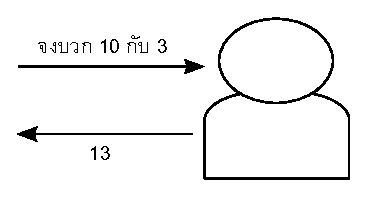
\epsfig{file=figures/recursion/add-call.eps, height=1in}
\end{center}
\caption{ตัวอย่าง{\wbr}การ{\wbr}เรียก{\wbr}ใช้{\wbr}โปรแกรมย่อย}
\label{rec:add-call}
\end{figure}

เรา{\wbr}จะ{\wbr}ปรับ{\wbr}โปรแกรมย่อย{\wbr}ดังกล่าว ให้{\wbr}เป็น{\wbr}โปรแกรมย่อย{\wbr}แบบ{\wbr}เรียก{\wbr}ตัวเอง{\wbr}
สมมติ{\wbr}ว่า{\wbr}เรา{\wbr}ทราบ{\wbr}วิธีการ{\wbr}เพิ่ม{\wbr}ค่า{\wbr}จำนวน{\wbr}ธรรมชาติ{\wbr}ขึ้น 1 และ{\wbr}ลด{\wbr}ค่า{\wbr}จำนวน{\wbr}ธรรมชาติ{\wbr}ลง 1
พิจารณา{\wbr}วิธีการ{\wbr}บวก{\wbr}จำนวน{\wbr}ธรรมชาติ $A$ เข้า{\wbr}กับ $B$
ดัง{\wbr}อัล{\wbr}กอ{\wbr}ริ{\wbr}ทึม{\wbr}ที่~\ref{algo:rec-int-add}

\begin{figure}
\begin{algt}
\label{algo:rec-int-add}
\noindent {\bf บวก{\wbr}จำนวน{\wbr}ธรรมชาติ $A$ กับ $B$}\\
\hspace*{0.2in} IF $B=0$ THEN RETURN $A$\\
\hspace*{0.2in} ELSE\\
\hspace*{0.2in}\hspace*{0.2in} LET $C\leftarrow B-1$\\
\hspace*{0.2in}\hspace*{0.2in} ให้ $D$ เท่า{\wbr}กับ{\wbr}ผลบวก{\wbr}ของ $A$ กับ $C$\\
\hspace*{0.2in}\hspace*{0.2in} RETURN $D+1$
\end{algt}
\end{figure}

นิยาม{\wbr}ข้างต้น{\wbr}มี{\wbr}ลักษณะ{\wbr}เหมือน{\wbr}งู{\wbr}กิน{\wbr}หาง{\wbr}
เพราะว่า{\wbr}เรา{\wbr}กำลัง{\wbr}นิยาม{\wbr}การ{\wbr}บวก{\wbr}จำนวน{\wbr}ธรรมชาติ{\wbr}ด้วย{\wbr}การ{\wbr}บวก{\wbr}จำนวน{\wbr}ธรรมชาติ อย่างไรก็ตาม{\wbr}
เรา{\wbr}จะ{\wbr}ละ{\wbr}ความ{\wbr}สงสัย{\wbr}ดังกล่าว{\wbr}ไว้{\wbr}ก่อน{\wbr}แล้ว{\wbr}ทดลอง{\wbr}บวก 10 กับ 3 ดังนี้{\wbr}

\begin{itemize}
\item เนื่องจาก $3$ ไม่{\wbr}เท่า{\wbr}กับ $0$ เรา{\wbr}จึง{\wbr}คำนวณ{\wbr}ค่า $3-1 = 2$
จากนั้น{\wbr}เรา{\wbr}ต้องการ{\wbr}คำนวณ{\wbr}หา{\wbr}ผลบวก{\wbr}ของ $10$ กับ $2$ เมื่อ{\wbr}ได้{\wbr}ผลบวก{\wbr}แล้ว เรา{\wbr}จะ{\wbr}เพิ่ม{\wbr}ค่า{\wbr}ขึ้น{\wbr}
$1$ เพื่อ{\wbr}ได้{\wbr}ผลบวก{\wbr}ของ $10$ กับ $3$ ตาม{\wbr}ต้องการ{\wbr}
\end{itemize}

\begin{figure}
\begin{center}
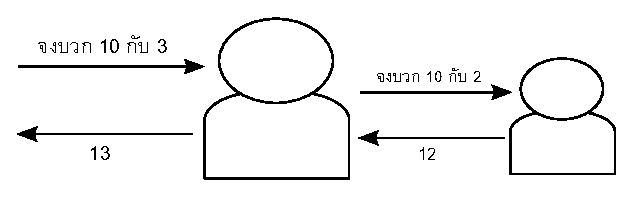
\epsfig{file=figures/recursion/add-2-calls.eps, height=1in}
\end{center}
\caption{ตัวอย่าง{\wbr}การ{\wbr}เรียก{\wbr}ใช้{\wbr}โปรแกรมย่อย{\wbr}ที่{\wbr}เรียก{\wbr}ใช้{\wbr}โปรแกรมย่อย{\wbr}เพื่อ{\wbr}คำนวณ{\wbr}ผลบวก{\wbr}ของ 10 กับ 2}
\label{rec:add-2-calls}
\end{figure}


จาก{\wbr}ขั้นตอน{\wbr}ด้าน{\wbr}บน ถ้า{\wbr}เรา{\wbr}ทราบ{\wbr}ว่า{\wbr}ผลบวก{\wbr}ของ $10$ กับ $2$ คือ $12$ เมื่อ{\wbr}เพิ่ม{\wbr}ค่า{\wbr}ขึ้น $1$
เรา{\wbr}จะ{\wbr}ได้{\wbr}ผลลัพธ์{\wbr}ของ $10$ กับ $3$ ซึ่ง{\wbr}มี{\wbr}ค่า{\wbr}เท่า{\wbr}กับ $13$ \ \ \
รูป~\ref{rec:add-2-calls} แสดง{\wbr}การ{\wbr}ทำงาน{\wbr}ของ{\wbr}โปรแกรมย่อย{\wbr}ดังกล่าว{\wbr}


\begin{quiz}{10 + 2}
เรา{\wbr}จะ{\wbr}หา{\wbr}ผลลัพธ์{\wbr}ของ{\wbr}การ{\wbr}บวก $10$ กับ $2$ ได้{\wbr}อย่างไร?
\end{quiz}

เรา{\wbr}ก็{\wbr}จะ{\wbr}หา{\wbr}ผลลัพธ์{\wbr}ด้วย{\wbr}วิธี{\wbr}เดียวกัน ซึ่ง{\wbr}ใน{\wbr}การ{\wbr}ผลบวก เรา{\wbr}จะ{\wbr}ต้องหา{\wbr}ผลลัพธ์{\wbr}ของ{\wbr}การ{\wbr}บวก $10$ กับ{\wbr}
$1$ และ{\wbr}จะ{\wbr}เป็น{\wbr}เช่นนี้{\wbr}เป็น{\wbr}เรื่อย ๆ ดัง{\wbr}ตัวอย่าง{\wbr}ด้าน{\wbr}ล่าง (รูป{\wbr}ที่~\ref{rec:add-rec-calls}
แสดง{\wbr}ลักษณะ{\wbr}การ{\wbr}คำนวณ)


\begin{itemize}
\item เนื่องจาก $3$ ไม่{\wbr}เท่า{\wbr}กับ $0$ เรา{\wbr}จึง{\wbr}คำนวณ{\wbr}ค่า $3-1 = 2$ จากนั้น{\wbr}เรา{\wbr}ต้องการ{\wbr}คำนวณ{\wbr}หา{\wbr}ผลบวก{\wbr}ของ $10$ กับ $2$ ใน{\wbr}การ{\wbr}คำนวณ{\wbr}ผลบวก{\wbr}ดังกล่าว เรา{\wbr}จะ{\wbr}ใช้{\wbr}วิธีการ{\wbr}เดิม{\wbr}
\begin{itemize}
\item เนื่องจาก $2$ ไม่{\wbr}เท่า{\wbr}กับ $0$ เรา{\wbr}จึง{\wbr}คำนวณ{\wbr}ค่า $2-1 = 1$ จากนั้น{\wbr}เรา{\wbr}ต้องการ{\wbr}คำนวณ{\wbr}หา{\wbr}ผลบวก{\wbr}ของ $10$ กับ $1$ ใน{\wbr}การ{\wbr}คำนวณ{\wbr}ผลบวก{\wbr}ดังกล่าว เรา{\wbr}จะ{\wbr}ใช้{\wbr}วิธีการ{\wbr}เดิม{\wbr}
\begin{itemize}
\item เนื่องจาก $1$ ไม่{\wbr}เท่า{\wbr}กับ $0$ เรา{\wbr}จึง{\wbr}คำนวณ{\wbr}ค่า $1-1 = 0$ จากนั้น{\wbr}เรา{\wbr}ต้องการ{\wbr}คำนวณ{\wbr}หา{\wbr}ผลบวก{\wbr}ของ $10$ กับ $0$ ใน{\wbr}การ{\wbr}คำนวณ{\wbr}ผลบวก{\wbr}ดังกล่าว เรา{\wbr}จะ{\wbr}ใช้{\wbr}วิธีการ{\wbr}เดิม{\wbr}
\begin{itemize}
\item เนื่องจาก $0$ เท่า{\wbr}กับ $0$ ผลลัพธ์{\wbr}ของ{\wbr}การ{\wbr}บวก $10$ กับ $0$ คือ $10$
\end{itemize}
\item เมื่อ{\wbr}เรา{\wbr}ได้{\wbr}ผลลัพธ์{\wbr}ของ{\wbr}การ{\wbr}บวก $10$ กับ $0$ แล้ว (คือ $10$) เรา{\wbr}คำนวณ $10+1$ ได้{\wbr}ผลลัพธ์ $11$ ซึ่ง{\wbr}เป็น{\wbr}ผลลัพธ์{\wbr}ของ{\wbr}การ{\wbr}บวก $10$ กับ $1$
\end{itemize}
\item เมื่อ{\wbr}เรา{\wbr}ได้{\wbr}ผลลัพธ์{\wbr}ของ{\wbr}การ{\wbr}บวก $10$ กับ $1$ แล้ว (คือ $11$) เรา{\wbr}คำนวณ $11+1$ ได้{\wbr}ผลลัพธ์ $12$ ซึ่ง{\wbr}เป็น{\wbr}ผลลัพธ์{\wbr}ของ{\wbr}การ{\wbr}บวก $10$ กับ $2$
\end{itemize}
\item เมื่อ{\wbr}เรา{\wbr}ได้{\wbr}ผลลัพธ์{\wbr}ของ{\wbr}การ{\wbr}บวก $10$ กับ $2$ แล้ว (คือ $12$) เรา{\wbr}คำนวณ $12+1$ ได้{\wbr}ผลลัพธ์ $13$ ซึ่ง{\wbr}เป็น{\wbr}ผลลัพธ์{\wbr}ของ{\wbr}การ{\wbr}บวก $10$ กับ $3$
\end{itemize}


\begin{figure}
\begin{center}
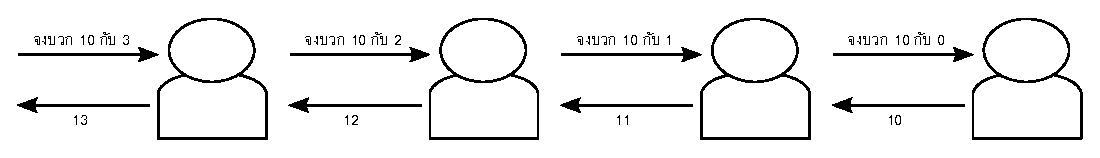
\epsfig{file=figures/recursion/add-rec-calls.eps, width=6in}
\end{center}
\caption{ตัวอย่าง{\wbr}การ{\wbr}เรียก{\wbr}ใช้{\wbr}โปรแกรมย่อย{\wbr}ที่{\wbr}เรียก{\wbr}ตัวเอง}
\label{rec:add-rec-calls}
\end{figure}


\begin{quiz}{การ{\wbr}ลบ}
เขียน{\wbr}ขั้นตอน{\wbr}การ{\wbr}ลบ{\wbr}จำนวน{\wbr}ธรรมชาติ $A$ กับ $B$ ใน{\wbr}รูปแบบ{\wbr}เดียวกับ{\wbr}การ{\wbr}คำนวณ{\wbr}ผลบวก{\wbr}
\end{quiz}

\begin{quiz}{การ{\wbr}คูณ}
เขียน{\wbr}ขั้นตอน{\wbr}การ{\wbr}คูณ{\wbr}จำนวน{\wbr}ธรรมชาติ $A$ กับ $B$ ใน{\wbr}รูปแบบ{\wbr}เดียวกับ{\wbr}การ{\wbr}คำนวณ{\wbr}ผลบวก{\wbr}
\end{quiz}

\begin{quiz}{ศูนย์}
ถ้า{\wbr}เรา{\wbr}ตัด{\wbr}บรรทัด{\wbr}แรก{\wbr}ที่{\wbr}ระบุ{\wbr}เงื่อนไข{\wbr}ที่ทำงาน{\wbr}เมื่อ $B=0$ ออก  เมื่อ{\wbr}เรา{\wbr}ดำเนินการ{\wbr}ตาม{\wbr}ขั้นตอนวิธี{\wbr}ดังกล่าว ผลลัพธ์{\wbr}จะ{\wbr}เป็น{\wbr}เช่น{\wbr}ใด{\wbr}
\end{quiz}

เรา{\wbr}สามารถ{\wbr}เขียน{\wbr}อัล{\wbr}กอ{\wbr}ริ{\wbr}ทึม{\wbr}ดังกล่าว{\wbr}เป็น{\wbr}โปรแกรม{\wbr}ได้{\wbr}ไม่{\wbr}ยาก{\wbr}ดังนี้{\wbr}

\latintext
\begin{codelist}{C++}{}
int add(int a, int b)
{
  if(b==0)
    return a;

  int c = b-1;
  return 1 + add(a,c);
}
\end{codelist}
\thaitext

\section{ค่าสูงสุด}

เรา{\wbr}จะ{\wbr}ออกแบบ{\wbr}อัล{\wbr}กอ{\wbr}ริ{\wbr}ทึม{\wbr}แบบ{\wbr}เรียก{\wbr}ตัวเอง{\wbr}สำหรับ{\wbr}การ{\wbr}คำนวณ{\wbr}ค่าสูงสุด กล่าวคือ{\wbr}
ให้{\wbr}อาร์เรย์ $A$ ของ{\wbr}จำนวนเต็ม $n$ จำนวน เรา{\wbr}ต้องการ{\wbr}คำนวณ{\wbr}ค่าสูงสุด{\wbr}

กรณี{\wbr}ที่{\wbr}เรา{\wbr}สามารถ{\wbr}ตอบ{\wbr}คำถาม{\wbr}ได้{\wbr}ง่าย คือ{\wbr}กรณี{\wbr}ที่ $n=1$
กล่าวคือ{\wbr}เรา{\wbr}สามารถ{\wbr}ตอบ{\wbr}ได้{\wbr}ทันที{\wbr}ว่า{\wbr}ค่าสูงสุด{\wbr}เท่า{\wbr}กับ $A[0]$

\begin{algt}
\noindent {\bf การ{\wbr}คำ{\wbr}น{\wbr}วน{\wbr}ค่าสูงสุด{\wbr}ของ{\wbr}อาร์เรย์ $A$ ที่{\wbr}มี{\wbr}สมาชิก $n$ ตัว (ขั้น{\wbr}ฐาน)}\\
\hspace*{0.2in} IF $n=1$ THEN RETURN $A[0]$\\
\hspace*{0.2in} ELSE\\
\hspace*{0.2in}\hspace*{0.2in} {\em จะ{\wbr}ต้อง{\wbr}ออกแบบ{\wbr}ต่อไป}
\end{algt}

สำหรับ{\wbr}บท{\wbr}นี้{\wbr}เพื่อ{\wbr}ความ{\wbr}สะดวก{\wbr}ใน{\wbr}การ{\wbr}เขียน{\wbr}
แทน{\wbr}ที่{\wbr}เรา{\wbr}จะ{\wbr}เรียก{\wbr}ข้อมูล{\wbr}ใน{\wbr}อาร์เรย์{\wbr}โดย{\wbr}เขียน{\wbr}ใน{\wbr}วงเล็บ{\wbr}เหลี่ยม เช่น $A[4]$ หรือ $A[i]$
เรา{\wbr}จะ{\wbr}เขียน{\wbr}เป็น{\wbr}ตัว{\wbr}ห้อย เช่น $A_4$ หรือ $A_i$
และ{\wbr}จะ{\wbr}เขียน{\wbr}อาร์เรย์{\wbr}โดย{\wbr}ระบุ{\wbr}ข้อมูล{\wbr}ใน{\wbr}อาร์เรย์{\wbr}ใน{\wbr}วงเล็บ{\wbr}เหลี่ยม เช่น อาร์เรย์
$[2,3,5,7,11]$ เป็นต้น{\wbr}

สำหรับ{\wbr}กรณี{\wbr}ทั่วไป เรา{\wbr}จะ{\wbr}เริ่ม{\wbr}โดย{\wbr}พิจารณา{\wbr}ปัญหา{\wbr}เมื่อ{\wbr}ข้อมูล{\wbr}นำเข้า{\wbr}มี{\wbr}ขนาด{\wbr}เล็ก{\wbr}ลง โดย{\wbr}เรา{\wbr}จะ{\wbr}ให้{\wbr}
\[
A' = [A_0,A_1,\ldots,A_{n-2}]
\]
นั่น{\wbr}คือ $A'$ คือ{\wbr}อาร์เรย์ $A$ ที่{\wbr}ตัด{\wbr}ข้อมูล{\wbr}ตัว{\wbr}สุดท้าย{\wbr}ทิ้ง{\wbr}ไป{\wbr}

ปัญหา{\wbr}นี้{\wbr}เรา{\wbr}จะ{\wbr}เรียก{\wbr}ว่า {\em ปัญหา{\wbr}ย่อย} (subproblem)
เรา{\wbr}จะ{\wbr}สมมติ{\wbr}ว่า{\wbr}เรา{\wbr}สามารถ{\wbr}หา{\wbr}คำตอบ{\wbr}ของ{\wbr}ปัญหา{\wbr}ได้ กล่าวคือ{\wbr}
ให้ $M$ คือ{\wbr}ค่าสูงสุด{\wbr}ของ{\wbr}อาร์เรย์ $A'$

\begin{quiz}{ค่า{\wbr}สูง{\wbr}ที่สุด{\wbr}จาก $M$}
สมมติ{\wbr}ว่า{\wbr}เรา{\wbr}ทราบ{\wbr}ว่า $M$ คือ{\wbr}ค่าสูงสุด{\wbr}ของ{\wbr}อาร์เรย์ $A'= [A_0,A_1,\ldots,A_{n-2}]$
เรา{\wbr}สามารถ{\wbr}คำนวณ{\wbr}ค่าสูงสุด{\wbr}ของ{\wbr}อาร์เรย์ 
$A= [A_0,A_1,\ldots,A_{n-1}]$
ได้{\wbr}อย่างไร?

(คำ{\wbr}ใบ้: ถ้า $M$ ไม่{\wbr}ใช่{\wbr}ข้อมูล{\wbr}ที่{\wbr}มี{\wbr}ค่าสูงสุด{\wbr}ของ{\wbr}อาร์เรย์ ค่า{\wbr}อื่น{\wbr}ที่{\wbr}เป็น{\wbr}ไป{\wbr}ได้{\wbr}คือ{\wbr}ค่า{\wbr}ใด?)
\end{quiz}

เมื่อ{\wbr}เรา{\wbr}พิจารณา{\wbr}ข้อมูล{\wbr}สูงสุด{\wbr}ของ{\wbr}อาร์เรย์ $A$ มี{\wbr}ความ{\wbr}เป็น{\wbr}ไป{\wbr}ได้{\wbr}สอง{\wbr}กรณี{\wbr}คือ{\wbr}
กรณี{\wbr}ที่{\wbr}ข้อมูล{\wbr}สูง{\wbr}ที่สุด{\wbr}อยู่{\wbr}ใน{\wbr}อาร์เรย์ $A'$ ใน{\wbr}อีก{\wbr}กรณี{\wbr}หนึ่ง{\wbr}คือ{\wbr}ข้อมูล{\wbr}สูง{\wbr}ที่สุด{\wbr}คือ $x_n$
ถ้า{\wbr}เป็น{\wbr}ใน{\wbr}กรณี{\wbr}แรก{\wbr}ค่าสูงสุด{\wbr}คือ $M$ ใน{\wbr}อีก{\wbr}กรณี{\wbr}หนึ่ง{\wbr}คือ ข้อมูล{\wbr}ตัว{\wbr}สุดท้าย $A_{n-1}$ ใน $A$
ซึ่ง{\wbr}เรา{\wbr}สามารถ{\wbr}เทียบ{\wbr}ข้อมูล{\wbr}ทั้ง{\wbr}สอง{\wbr}เพื่อ{\wbr}หา{\wbr}ค่า{\wbr}สูง{\wbr}ที่สุด{\wbr}ได้ ดัง{\wbr}อัล{\wbr}กอ{\wbr}ริ{\wbr}ทึม{\wbr}ด้าน{\wbr}ล่าง{\wbr}

\begin{algt}
\label{}
\noindent {\bf การ{\wbr}คำ{\wbr}น{\wbr}วน{\wbr}ค่าสูงสุด{\wbr}ของ{\wbr}อาร์เรย์ $A$ ที่{\wbr}มี{\wbr}สมาชิก $n$ ตัว}\\
1.\settowidth{\algbackindent}{1.}\hspace*{-\algbackindent}\hspace*{0.2in} IF $n=1$ THEN RETURN $A[0]$\\
2.\settowidth{\algbackindent}{2.}\hspace*{-\algbackindent}\hspace*{0.2in} ELSE\\
3.\settowidth{\algbackindent}{3.}\hspace*{-\algbackindent}\hspace*{0.2in}\hspace*{0.2in} ให้ $M$ คือ{\wbr}ค่าสูงสุด{\wbr}ของ{\wbr}อาร์เรย์ $A'$ ที่{\wbr}มี{\wbr}สมาชิก $n-1$ ตัว เมื่อ $A' = [A_0,A_1,\ldots,A_{n-2}]$\\
4.\settowidth{\algbackindent}{4.}\hspace*{-\algbackindent}\hspace*{0.2in}\hspace*{0.2in} IF $A_{n-1} > M$ THEN \\
5.\settowidth{\algbackindent}{5.}\hspace*{-\algbackindent}\hspace*{0.2in}\hspace*{0.2in}\hspace*{0.2in} RETURN $A_{n-1}$\\
6.\settowidth{\algbackindent}{6.}\hspace*{-\algbackindent}\hspace*{0.2in}\hspace*{0.2in} ELSE\\
7.\settowidth{\algbackindent}{7.}\hspace*{-\algbackindent}\hspace*{0.2in}\hspace*{0.2in}\hspace*{0.2in} RETURN $M$
\end{algt}

คำถาม{\wbr}ก็{\wbr}คือ ใน{\wbr}ขั้นตอน{\wbr}ที่ 3 เรา{\wbr}จะ{\wbr}คำนวณ{\wbr}หา{\wbr}ค่า $M$ ได้{\wbr}อย่างไร?
สังเกต{\wbr}ว่า{\wbr}ปัญหา{\wbr}ดังกล่าว{\wbr}ก็{\wbr}คือ{\wbr}ปัญหา{\wbr}เดียวกับ{\wbr}ปัญหา{\wbr}เริ่มต้น{\wbr}ที่{\wbr}เรา{\wbr}ต้องการ{\wbr}จะ{\wbr}แก้{\wbr}
แต่{\wbr}มี{\wbr}ข้อมูล{\wbr}ป้อน{\wbr}เข้าที่{\wbr}แตกต่าง{\wbr}ออก{\wbr}ไป ดังนั้น ใน{\wbr}การ{\wbr}แก้{\wbr}ปัญหา{\wbr}ดังกล่าว{\wbr}
เรา{\wbr}ก็{\wbr}จะ{\wbr}เรียก{\wbr}ฟังก์ชัน{\wbr}ที่{\wbr}เรา{\wbr}เตรียม{\wbr}ไว้{\wbr}สำหรับ{\wbr}แก้{\wbr}ปัญหา{\wbr}นั้น นั่น{\wbr}ก็{\wbr}คือ{\wbr}ฟังก์ชัน{\wbr}ที่{\wbr}เรา{\wbr}กำลัง{\wbr}เขียน{\wbr}อยู่{\wbr}นั่นเอง{\wbr}

จาก{\wbr}แนว{\wbr}คิด{\wbr}ดังกล่าว เรา{\wbr}สามารถ{\wbr}พัฒนา{\wbr}โปรแกรม{\wbr}ที่{\wbr}คำนวณ{\wbr}ค่าสูงสุด{\wbr}ได้{\wbr}ดังนี้{\wbr}

\latintext
\begin{codelist}{C++}{}
int arraymax(int ar[], int n)
{
  if(n==1)
    return ar[0];
  else {
    int m = arraymax(ar,n-1);   // Line 6
    if(m > xn)
      return m;
    else
      return ar[n-1];
  }
}
\end{codelist}
\thaitext

สังเกต{\wbr}ว่า{\wbr}ใน{\wbr}โปรแกรม{\wbr}ดังกล่าว เรา{\wbr}ไม่{\wbr}ได้{\wbr}สร้าง{\wbr}อาร์เรย์ $A'$ ขึ้น{\wbr}มา{\wbr}ใหม่{\wbr}แต่อย่างใด{\wbr}
เนื่องจาก{\wbr}วิธีการ{\wbr}เรา{\wbr}สามารถ{\wbr}พิจารณา{\wbr}ให้ $A'$ เป็น{\wbr}แค่{\wbr}ส่วน{\wbr}ต้น{\wbr}ของ{\wbr}อาร์เรย์ $A$
สิ่ง{\wbr}ที่{\wbr}เรา{\wbr}ทำ{\wbr}เพื่อ{\wbr}ป้อน{\wbr}เป็น{\wbr}ข้อมูล{\wbr}ป้อน{\wbr}เข้า{\wbr}ให้{\wbr}กับ{\wbr}ฟังก์ชัน {\ct arraymax}
คือ{\wbr}ปรับ{\wbr}จำนวน{\wbr}ของ{\wbr}ข้อมูล{\wbr}ใน{\wbr}อาร์เรย์{\wbr}เท่านั้น{\wbr}เอง{\wbr}

\begin{quiz}{ผลบวก{\wbr}ของ{\wbr}อาร์เรย์}
ออกแบบ{\wbr}อัล{\wbr}กอ{\wbr}ริ{\wbr}ทึม{\wbr}ที่{\wbr}รับ{\wbr}อาร์เรย์ $A$ ของ{\wbr}จำนวนเต็ม $n$ จำนวน{\wbr}
แล้ว{\wbr}คำนวณ{\wbr}ผลรวม{\wbr}ของ{\wbr}ข้อมูล{\wbr}ใน{\wbr}รายการ{\wbr}
\end{quiz}

\begin{quiz}{เปลี่ยน{\wbr}ทิศทาง}
แทน{\wbr}ที่{\wbr}เรา{\wbr}จะ{\wbr}นิยาม{\wbr}ให้ $A'$ เป็น{\wbr}อาร์เรย์ $A$ ที่{\wbr}ลบ{\wbr}ข้อมูล{\wbr}ตัว{\wbr}สุดท้าย{\wbr}ออก{\wbr}ไป เรา{\wbr}อาจ{\wbr}จะ{\wbr}นิยาม{\wbr}
\[
A'=[A_1,A_2,\ldots,A_{n-1}]
\]
นั่น{\wbr}คือ ให้{\wbr}เป็น{\wbr}อาร์เรย์ $A$ ที่{\wbr}ลบ{\wbr}ข้อมูล{\wbr}ตัว{\wbr}แรก{\wbr}ออก{\wbr}
จง{\wbr}พัฒนา{\wbr}อัล{\wbr}กอ{\wbr}ริ{\wbr}ทึม{\wbr}หา{\wbr}ค่า{\wbr}มาก{\wbr}ที่สุด{\wbr}โดย{\wbr}ใช้{\wbr}การ{\wbr}เรียก{\wbr}ตัวเอง{\wbr}บน{\wbr}อาร์เรย์ $A'$ ที่{\wbr}นิยาม{\wbr}ใหม่{\wbr}นี้{\wbr}
และ{\wbr}เขียน{\wbr}โปรแกรม{\wbr}

(คำแนะนำ{\wbr}เพิ่มเติม: ใน{\wbr}การ{\wbr}ส่ง{\wbr}ค่า $A'$ ใน{\wbr}การ{\wbr}เรียก{\wbr}ตัวเอง{\wbr}อาจ{\wbr}จะ{\wbr}ดู{\wbr}ซับซ้อน{\wbr}กว่า{\wbr}วิธี{\wbr}เก่า{\wbr}เล็กน้อย{\wbr}
แต่{\wbr}อย่า{\wbr}ลืม{\wbr}ว่า{\wbr}เรา{\wbr}สามารถ{\wbr}บวก{\wbr}พอยน์เตอร์{\wbr}ได้)
\end{quiz}



\subsection{ฟังก์ชัน{\wbr}เรียก{\wbr}ตัวเอง}
อัล{\wbr}กอ{\wbr}ริ{\wbr}ทึม{\wbr}ดังกล่าว{\wbr}สามารถ{\wbr}พิจารณา{\wbr}ว่า{\wbr}เป็น{\wbr}การ{\wbr}คำนวณ{\wbr}ค่า{\wbr}ฟังก์ชัน $f$ ที่{\wbr}มี{\wbr}นิยาม{\wbr}ดังต่อไปนี้{\wbr}

$f([A_0,A_1,\ldots,A_{n-1}]) = 
\left\{
\begin{array}{ll}
A_0, &  \mbox{ถ้า } n=1 \\
\max \{ A_{n-1},f([A_0,A_1,\ldots,A_{n-2}]) \},  & \mbox{ใน{\wbr}กรณี{\wbr}อื่น ๆ}
\end{array}
\right.$

\subsection{การ{\wbr}ทำ{\wbr}ซ้ำ{\wbr}กับ{\wbr}การ{\wbr}เรียก{\wbr}ตัวเอง}
การ{\wbr}คำนวณ{\wbr}ค่าสูงสุด{\wbr}ใน{\wbr}รายการ{\wbr}เป็น{\wbr}ปัญหา{\wbr}พื้นฐาน{\wbr}ที่{\wbr}เหมาะ{\wbr}กับ{\wbr}อัล{\wbr}กอ{\wbr}ริ{\wbr}ทึม{\wbr}แบบ{\wbr}ทำ{\wbr}ซ้ำ{\wbr}
ด้าน{\wbr}ล่าง{\wbr}แสดง{\wbr}ส่วน{\wbr}ของ{\wbr}โปรแกรม{\wbr}ดังกล่าว{\wbr}

\latintext
\begin{codelist}{C++}{}
int arraymax(int ar[], int n)
{
  int m = ar[0];
  for(int i=0; i<n; ++i)
    if(ar[i] > m)
      m = ar[i];
  return m;
}
\end{codelist}
\thaitext

ผู้อ่าน{\wbr}ที่{\wbr}สนใจ{\wbr}อาจ{\wbr}เริ่ม{\wbr}สงสัย{\wbr}ว่า{\wbr}การ{\wbr}พัฒนา{\wbr}โปรแกรม{\wbr}แบบ{\wbr}เรียก{\wbr}ตัวเอง{\wbr}มี{\wbr}ประโยชน์{\wbr}อย่างไร?

TODO: อธิบาย{\wbr}เพิ่มเติม{\wbr}

อย่างไรก็ตาม ภาษา{\wbr}โปรแกรม{\wbr}ภายใต้{\wbr}กรอบ{\wbr}คิด{\wbr}ที่{\wbr}ไม่{\wbr}ใช่{\wbr}ภาษา{\wbr}เชิง imperative
อาจ{\wbr}จะ{\wbr}ไม่{\wbr}มี{\wbr}โครงสร้าง{\wbr}ควบคุม{\wbr}ที่{\wbr}เป็น{\wbr}การ{\wbr}วน{\wbr}รอบ เช่น ภาษา{\wbr}เชิง{\wbr}ฟังก์ชัน เช่น Haskell หรือ ML
หรือ{\wbr}ภาษา{\wbr}เชิง{\wbr}ตรรก เช่น Prolog โปรแกรม{\wbr}ที่{\wbr}เขียน{\wbr}บน{\wbr}ภาษา{\wbr}ใน{\wbr}กลุ่ม{\wbr}นี้{\wbr}
จะ{\wbr}ไม่{\wbr}มี{\wbr}แนว{\wbr}คิด{\wbr}เกี่ยวกับ{\wbr}การ{\wbr}เปลี่ยนแปลง{\wbr}ค่า{\wbr}ของ{\wbr}ตัวแปร{\wbr}
จึง{\wbr}ทำ{\wbr}ให้{\wbr}โปรแกรม{\wbr}ที่{\wbr}เขียน{\wbr}ปราศจาก{\wbr}ผลข้างเคียง (side effect)
ทั้งหมด{\wbr}นี้{\wbr}ทำ{\wbr}ให้{\wbr}สามารถ{\wbr}ทดสอบ{\wbr}โปรแกรม{\wbr}สะดวก{\wbr}ขึ้น ลด{\wbr}ข้อผิดพลาด{\wbr}
และ{\wbr}ทำ{\wbr}ให้{\wbr}โปรแกรม{\wbr}สามารถ{\wbr}ทำงาน{\wbr}แบบ{\wbr}ขนาน{\wbr}ได้{\wbr}ง่าย{\wbr}ขึ้น{\wbr}ด้วย{\wbr}


\section{การ{\wbr}จัดเรียง{\wbr}ข้อมูล}

ใน{\wbr}ส่วน{\wbr}นี้{\wbr}เรา{\wbr}จะ{\wbr}พิจารณา{\wbr}ตัวอย่าง{\wbr}การ{\wbr}ออกแบบ{\wbr}อัล{\wbr}กอ{\wbr}ริ{\wbr}ทึม{\wbr}โดย{\wbr}การ{\wbr}คิด{\wbr}แบบ{\wbr}เรียก{\wbr}ตัวเอง{\wbr}
ปัญหา{\wbr}ที่{\wbr}เรา{\wbr}สนใจ{\wbr}คือ{\wbr}ปัญหา{\wbr}การ{\wbr}จัดเรียง{\wbr}ข้อมูล ซึ่ง{\wbr}เป็น{\wbr}ปัญหา{\wbr}เกี่ยวกับ{\wbr}การ{\wbr}ประมวลผล{\wbr}ข้อมูล{\wbr}ที่{\wbr}สำคัญ{\wbr}มาก{\wbr}

เรา{\wbr}มี{\wbr}จำนวนเต็ม $n$ จำนวน อยู่{\wbr}ใน{\wbr}อาร์เรย์ $x$ (นั่น{\wbr}คือ{\wbr}ข้อมูล{\wbr}คือ{\wbr}
$[x_0,x_1,\ldots,x_{n-1}]$) เรา{\wbr}ต้องการ{\wbr}เรียง{\wbr}ข้อมูล{\wbr}ใน{\wbr}อาร์เรย์{\wbr}ดังกล่าว{\wbr}จาก{\wbr}น้อย{\wbr}ไป{\wbr}มาก{\wbr}

\begin{quiz}{กรณี{\wbr}ง่าย}
มี{\wbr}กรณี{\wbr}ใด{\wbr}บ้าง{\wbr}ที่{\wbr}เรา{\wbr}สามารถ{\wbr}เรียง{\wbr}ข้อมูล{\wbr}ใน{\wbr}อาร์เรย์ $x$ ได้{\wbr}ง่าย{\wbr}มาก{\wbr}
\end{quiz}

กรณี{\wbr}ที่{\wbr}อาร์เรย์{\wbr}มี{\wbr}ข้อมูล{\wbr}เพียง 1 จำนวน การ{\wbr}จัดเรียง{\wbr}อาร์เรย์{\wbr}ดังกล่าว{\wbr}สามารถ{\wbr}ทำ{\wbr}ได้{\wbr}โดย{\wbr}ง่าย นั่น{\wbr}คือ{\wbr}
ไม่{\wbr}ต้อง{\wbr}ทำ{\wbr}อะไร{\wbr}เลย  ถ้า{\wbr}ไม่{\wbr}ใช่{\wbr}กรณี{\wbr}ดังกล่าว เรา{\wbr}จะ{\wbr}เรียง{\wbr}ข้อมูล{\wbr}ได้{\wbr}อย่างไร?

แทน{\wbr}ที่{\wbr}จะ{\wbr}เริ่ม{\wbr}แบบ{\wbr}ไม่{\wbr}มี{\wbr}อะไร{\wbr}เลย เรา{\wbr}จะ{\wbr}สมมติ{\wbr}ว่า{\wbr}ใน{\wbr}การ{\wbr}พัฒนา{\wbr}โปรแกรม{\wbr}ใน{\wbr}การ{\wbr}จัดการ{\wbr}เรียง{\wbr}ข้อมูล{\wbr}
$n$ ตัว เรา{\wbr}สามารถ{\wbr}เรียง{\wbr}ข้อมูล{\wbr}ใน{\wbr}อาร์เรย์{\wbr}ที่{\wbr}มี{\wbr}ข้อมูล{\wbr}จำนวน $m$ ตัว{\wbr}ได้{\wbr}

สังเกต{\wbr}ว่า{\wbr}เรา{\wbr}กำลัง{\wbr}แก้{\wbr}ปัญหา{\wbr}การ{\wbr}จัดเรียง{\wbr}ข้อมูล แต่{\wbr}เรา{\wbr}สมมติ{\wbr}ว่า{\wbr}เรา{\wbr}แก้{\wbr}ปัญหา{\wbr}นั้น{\wbr}ได้{\wbr}แล้ว!
ถ้า{\wbr}สมมติ{\wbr}กัน{\wbr}ได้{\wbr}ง่าย ๆ แบบ{\wbr}นี้{\wbr}โปรแกรม{\wbr}ที่{\wbr}ใช้{\wbr}เรียง{\wbr}ข้อมูล{\wbr}ของ{\wbr}เรา{\wbr}คง{\wbr}มี{\wbr}ลักษณะ{\wbr}ดังนี้{\wbr}

\begin{algt}
\noindent {\bf เรียง{\wbr}ข้อมูล{\wbr}ใน{\wbr}อาร์เรย์ $x$ ที่{\wbr}มี{\wbr}ข้อมูล $n$ ตัว}\\
\hspace*{0.2in} เรียง{\wbr}ข้อมูล{\wbr}ใน{\wbr}อาร์เรย์ $x$ ที่{\wbr}มี{\wbr}ข้อมูล $n$ ตัว\\
\hspace*{0.2in} คืน{\wbr}ผลลัพธ์{\wbr}
\end{algt}

\begin{quiz}{อัล{\wbr}กอ{\wbr}ริ{\wbr}ทึม{\wbr}สมมติ}
อัล{\wbr}กอ{\wbr}ริ{\wbr}ทึม{\wbr}ดังกล่าว{\wbr}ทำงาน{\wbr}ได้{\wbr}จริง{\wbr}หรือ{\wbr}ไม่? เพราะ{\wbr}เหตุใด?
\end{quiz}

อัล{\wbr}กอ{\wbr}ริ{\wbr}ทึม{\wbr}ข้างต้น{\wbr}นั้น{\wbr}ทำงาน{\wbr}ไม่{\wbr}ได้{\wbr}จริง{\wbr}
เพราะว่า{\wbr}การ{\wbr}ทำงาน{\wbr}ของ{\wbr}อัล{\wbr}กอ{\wbr}ริ{\wbr}ทึม{\wbr}จะ{\wbr}เป็น{\wbr}การ{\wbr}เรียก{\wbr}ตัวเอง{\wbr}ไป{\wbr}เรื่อย ๆ ไม่{\wbr}มี{\wbr}วัน{\wbr}สิ้นสุด{\wbr}

ดังนั้น{\wbr}การ{\wbr}สมมติ{\wbr}ว่า{\wbr}เรา{\wbr}สามารถ{\wbr}เรียง{\wbr}ข้อมูล{\wbr}ใน{\wbr}อาร์เรย์{\wbr}ได้{\wbr}นั้น จึง{\wbr}ต้อง{\wbr}มี{\wbr}ขอบเขต{\wbr}ที่{\wbr}ก่อ{\wbr}ให้{\wbr}เกิด{\wbr}
`{\wbr}`{\wbr}ความ{\wbr}ก้าวหน้า'' ของ{\wbr}การ{\wbr}ทำงาน{\wbr}
ใน{\wbr}ที่นี้{\wbr}เรา{\wbr}จะ{\wbr}ใส่{\wbr}เงื่อนไข{\wbr}เพิ่มเติม{\wbr}ว่า{\wbr}ขนาด{\wbr}ของ{\wbr}อาร์เรย์{\wbr}ที่{\wbr}เรา{\wbr}สามารถ{\wbr}สมมติ{\wbr}ว่า{\wbr}เรียง{\wbr}ได้{\wbr}นั้น{\wbr}มี{\wbr}ค่า{\wbr}ไม่{\wbr}เกิน{\wbr}
$n-1$ หรือ{\wbr}ให้ $m < n$

ดังนั้น{\wbr}เป้าหมาย{\wbr}ของ{\wbr}เรา{\wbr}จะ{\wbr}เปลี่ยน{\wbr}จาก{\wbr}การ{\wbr}พยายาม{\wbr}เรียง{\wbr}ข้อมูล $n$ ตัว{\wbr}
ไป{\wbr}เป็น{\wbr}การ{\wbr}พยายาม{\wbr}ทำงาน{\wbr}บาง{\wbr}อย่าง เพื่อ{\wbr}ทำ{\wbr}ให้{\wbr}งาน{\wbr}ที่{\wbr}เหลือก{\wbr}ลาย{\wbr}เป็น{\wbr}ปัญหา{\wbr}การ{\wbr}เรียง{\wbr}ข้อมูล $m$
ตัว โดย{\wbr}ที่ $m<n$

\begin{quiz}{แนวทาง{\wbr}การ{\wbr}แก้{\wbr}ปัญหา}
แนวทาง{\wbr}ที่{\wbr}เรา{\wbr}ระบุ{\wbr}ใน{\wbr}ย่อหน้า{\wbr}ข้างต้น{\wbr}ไม่{\wbr}ใช่{\wbr}แนวทาง{\wbr}เดียว{\wbr}ใน{\wbr}การ{\wbr}คิด{\wbr}แบบ{\wbr}เรียก{\wbr}ตัวเอง มี{\wbr}แนวทาง{\wbr}อื่น{\wbr}อีก{\wbr}หรือ{\wbr}ไม่?

(คำ{\wbr}ใบ้: สลับ)
\end{quiz}

เรา{\wbr}จะ{\wbr}ได้{\wbr}พิจารณา{\wbr}แนวทาง{\wbr}อื่น{\wbr}ใน{\wbr}การ{\wbr}คิด{\wbr}แบบ{\wbr}เรียก{\wbr}ตัวเอง{\wbr}ใน{\wbr}ตัวอย่าง{\wbr}ถัด ๆ ไป  

สำหรับ{\wbr}ปัญหา{\wbr}การ{\wbr}จัดเรียง{\wbr}ข้อมูล{\wbr}นี้ เรา{\wbr}จะ{\wbr}เริ่ม{\wbr}โดย{\wbr}การ{\wbr}พยายาม{\wbr}หา{\wbr}คำตอบ{\wbr}บาง{\wbr}ส่วน{\wbr}ให้{\wbr}ได้{\wbr}
เพื่อที่จะ{\wbr}ได้{\wbr}ทำ{\wbr}ให้{\wbr}งาน{\wbr}ที่{\wbr}เหลือ{\wbr}ลด{\wbr}ลง{\wbr}

\begin{quiz}{คำตอบ{\wbr}บาง{\wbr}ส่วน}
คำตอบ{\wbr}บาง{\wbr}ส่วน{\wbr}ของ{\wbr}ปัญหา{\wbr}การ{\wbr}เรียง{\wbr}ข้อมูล{\wbr}มี{\wbr}ได้{\wbr}หลาย{\wbr}แบบ ลอง{\wbr}ยก{\wbr}ตัวอย่าง{\wbr}สัก 2 แบบ{\wbr}
\end{quiz}

ใน{\wbr}ที่นี้{\wbr}เรา{\wbr}จะ{\wbr}พยายาม{\wbr}ทำ{\wbr}ให้{\wbr}ข้อมูล{\wbr}บาง{\wbr}ตัว{\wbr}ใน{\wbr}อาร์เรย์ อยู่{\wbr}ใน{\wbr}ตำแหน่ง ``ที่{\wbr}ถูกต้อง'' นั่น{\wbr}คือ{\wbr}
ตำแหน่ง{\wbr}ที่{\wbr}ข้อมูล{\wbr}นั้น{\wbr}จะ{\wbr}อยู่{\wbr}เมื่อ{\wbr}อาร์เรย์{\wbr}ดังกล่าว{\wbr}ถูก{\wbr}เรียง{\wbr}แล้ว  

\begin{quiz}{ตำแหน่ง{\wbr}ที่{\wbr}ถูกต้อง}
สมมติ{\wbr}เรา{\wbr}พิจารณา{\wbr}ข้อมูล $x_0$ จะ{\wbr}หา{\wbr}ตำแหน่ง{\wbr}ที่{\wbr}ถูกต้อง{\wbr}ของ $x_0$ ได้{\wbr}อย่างไร?
\end{quiz}

แทน{\wbr}ที่{\wbr}เรา{\wbr}จะ{\wbr}เริ่มต้น{\wbr}ด้วย{\wbr}ข้อมูล{\wbr}บาง{\wbr}ตัว เช่น $x_0$ แล้ว{\wbr}หา{\wbr}ตำแหน่ง{\wbr}ที่{\wbr}ถูกต้อง{\wbr}
เรา{\wbr}อาจ{\wbr}จะ{\wbr}มอง{\wbr}กลับ{\wbr}กัน คือ{\wbr}เริ่ม{\wbr}ที่{\wbr}ตำแหน่ง{\wbr}บาง{\wbr}ตำแหน่ง แล้ว{\wbr}หา{\wbr}ข้อมูล{\wbr}ที่{\wbr}ควร{\wbr}จะ{\wbr}อยู่{\wbr}ใน{\wbr}ตำแหน่ง{\wbr}ดังกล่าว{\wbr}

\begin{quiz}{ข้อมูล{\wbr}ถูกต้อง}
(1) เรา{\wbr}จะ{\wbr}หา{\wbr}ข้อมูล{\wbr}ที่{\wbr}ควร{\wbr}จะ{\wbr}มี{\wbr}ดัชนี{\wbr}เท่า{\wbr}กับ $0$ ใน{\wbr}อาร์เรย์{\wbr}ที่{\wbr}เรียง{\wbr}แล้ว{\wbr}ได้{\wbr}อย่างไร?  (2)
เรา{\wbr}จะ{\wbr}หา{\wbr}ข้อมูล{\wbr}ที่{\wbr}ควร{\wbr}จะ{\wbr}มี{\wbr}ดัชนี{\wbr}เท่า{\wbr}กับ $n-1$ ใน{\wbr}อาร์เรย์{\wbr}ที่{\wbr}เรียง{\wbr}แล้ว{\wbr}ได้{\wbr}อย่างไร?
\end{quiz}

\section{การ{\wbr}อุปนัย{\wbr}เชิง{\wbr}คณิตศาสตร์}

ใน{\wbr}การ{\wbr}พัฒนา{\wbr}โปรแกรม{\wbr}ใด ๆ สิ่ง{\wbr}ที่{\wbr}เรา{\wbr}ต้อง{\wbr}สนใจ{\wbr}ก่อน{\wbr}ที่{\wbr}จะ{\wbr}พิจารณา{\wbr}ถึง{\wbr}ประสิทธิภาพ{\wbr}ของ{\wbr}โปรแกรม{\wbr}
ก็{\wbr}คือ{\wbr}ความ{\wbr}ถูกต้อง{\wbr}ของ{\wbr}โปรแกรม{\wbr}นั้น ๆ อย่างไรก็ตาม{\wbr}
การ{\wbr}พิสูจน์{\wbr}ความ{\wbr}ถูกต้อง{\wbr}ของ{\wbr}โปรแกรมย่อย{\wbr}แบบ{\wbr}เรียก{\wbr}ตัวเอง{\wbr}นั้น{\wbr}มี{\wbr}ความ{\wbr}ซับซ้อน{\wbr}เป็นพิเศษ{\wbr}
ขั้นตอน{\wbr}การ{\wbr}ทำงาน{\wbr}ทั้งหมด{\wbr}มัก{\wbr}ไม่{\wbr}ได้{\wbr}ถูก{\wbr}ระบุ{\wbr}ออก{\wbr}มา{\wbr}อย่าง{\wbr}ชัดเจน{\wbr}ภายใน{\wbr}โปรแกรมย่อย{\wbr}นั้น{\wbr}
แต่{\wbr}จะ{\wbr}เป็น{\wbr}การ{\wbr}โยน{\wbr}ภาระ{\wbr}การ{\wbr}ทำงาน{\wbr}ให้{\wbr}กับ{\wbr}โปรแกรมย่อย{\wbr}นั้น{\wbr}เอง{\wbr}

ใน{\wbr}ส่วน{\wbr}นี้{\wbr}เรา{\wbr}จะ{\wbr}ศึกษา{\wbr}เกี่ยวกับ{\wbr}เทคนิค{\wbr}การ{\wbr}พิสูจน์{\wbr}ที่{\wbr}เรียก{\wbr}ว่า {\em การ{\wbr}อุปนัย{\wbr}ทาง{\wbr}คณิตศาสตร์}
(mathematical induction)
ซึ่ง{\wbr}เป็น{\wbr}เครื่องมือ{\wbr}สำคัญ{\wbr}ใน{\wbr}การ{\wbr}พิสูจน์{\wbr}ความ{\wbr}ถูกต้อง{\wbr}ของ{\wbr}โปรแกรมย่อย{\wbr}แบบ{\wbr}เรียก{\wbr}ตัวเอง{\wbr}

เรา{\wbr}จะ{\wbr}เริ่ม{\wbr}จาก{\wbr}ตัวอย่าง พิจารณา{\wbr}ผลรวม $1+2+3+\cdots+n$ ถ้า{\wbr}ยัง{\wbr}พอ{\wbr}จำ{\wbr}ได้{\wbr}
ผลรวม{\wbr}ดังกล่าว{\wbr}มี{\wbr}ค่า{\wbr}เท่า{\wbr}กับ $\frac{n(n+1)}{2}$
อย่างไรก็ตาม{\wbr}เรา{\wbr}จะ{\wbr}พิสูจน์{\wbr}ได้{\wbr}อย่างไร{\wbr}ว่า{\wbr}ผลรวม{\wbr}ดังกล่าว{\wbr}มี{\wbr}ค่า{\wbr}เท่า{\wbr}กับ{\wbr}นิพจน์{\wbr}ที่{\wbr}อ้าง{\wbr}มา{\wbr}จริง{\wbr}

เรา{\wbr}อาจ{\wbr}ทดลอง{\wbr}ได้{\wbr}โดย{\wbr}การ{\wbr}แทน{\wbr}ค่า $ n $ ด้วย{\wbr}ค่า{\wbr}ต่าง ๆ เช่น{\wbr}

\begin{itemize}
\item เมื่อ $ n=1 $ เรา{\wbr}จะ{\wbr}ได้{\wbr}ว่า{\wbr}ผลรวม{\wbr}ข้างต้น{\wbr}มี{\wbr}ค่า{\wbr}เท่า{\wbr}กับ $ 1 $ ใน{\wbr}ขณะที่{\wbr}นิพจน์ $
  \frac{n(n+1)}{2}=\frac{1\cdot 2}{2}=1 $ เช่นกัน{\wbr}
\item เมื่อ $ n=2 $ เรา{\wbr}จะ{\wbr}ได้{\wbr}ว่า ผลรวม{\wbr}มี{\wbr}ค่า $ 1+2=3 $ ใน{\wbr}ขณะที่ $
  \frac{n(n+1)}{2}=\frac{2\cdot 3}{2}=3 $ เช่นกัน{\wbr}
\end{itemize}

เรา{\wbr}สามารถ{\wbr}ไล่{\wbr}แทน{\wbr}ค่า{\wbr}ไป{\wbr}ได้{\wbr}เรื่อย ๆ
... อย่างไรก็ตาม{\wbr}วิธี{\wbr}ดังกล่าว{\wbr}ไม่{\wbr}สามารถ{\wbr}พิสูจน์{\wbr}ได้{\wbr}ว่า{\wbr}ผลรวม{\wbr}มี{\wbr}ค่า{\wbr}เท่า{\wbr}กับ{\wbr}นิพจน์{\wbr}ที่{\wbr}อ้าง{\wbr}มา{\wbr}ได้{\wbr}
เนื่องจาก{\wbr}อาจ{\wbr}มี{\wbr}ค่า{\wbr}บาง{\wbr}ค่า{\wbr}ที่{\wbr}เรา{\wbr}ไม่{\wbr}ได้{\wbr}แทน{\wbr}ลง{\wbr}ไป{\wbr}ที่{\wbr}ผลรวม{\wbr}มี{\wbr}ค่า{\wbr}ไม่{\wbr}เท่า{\wbr}กับ{\wbr}นิพจน์{\wbr}ดังกล่าว{\wbr}

ใน{\wbr}การ{\wbr}พิสูจน์{\wbr}โดย{\wbr}ทั่วไป หลาย{\wbr}ครั้ง{\wbr}เรา{\wbr}จะ{\wbr}เริ่ม{\wbr}จาก{\wbr}สิ่ง{\wbr}ที่{\wbr}เรา{\wbr}ทราบ{\wbr}
จากนั้น{\wbr}จะ{\wbr}ใช้{\wbr}เหตุผล{\wbr}เพื่อ{\wbr}เชื่อมโยง{\wbr}ให้{\wbr}ได้{\wbr}ผลลัพธ์{\wbr}ตาม{\wbr}ที่{\wbr}เรา{\wbr}ต้องการ{\wbr}
และ{\wbr}ใน{\wbr}บาง{\wbr}ครั้ง{\wbr}เรา{\wbr}ก็{\wbr}จะ{\wbr}เริ่ม{\wbr}จาก{\wbr}ผล{\wbr}ที่{\wbr}เรา{\wbr}ต้องการ{\wbr}
แล้ว{\wbr}จึง{\wbr}พยายาม{\wbr}โยง{\wbr}สิ่ง{\wbr}ที่{\wbr}เรา{\wbr}ทราบ{\wbr}มา{\wbr}หา{\wbr}ผล{\wbr}ดังกล่าว{\wbr}โดย{\wbr}ใช้{\wbr}ลำดับ{\wbr}การ{\wbr}ให้{\wbr}เหตุผล{\wbr}ที่{\wbr}ถูกต้อง{\wbr}

การ{\wbr}อุปนัย{\wbr}ทาง{\wbr}คณิตศาสตร์ นั้น{\wbr}มี{\wbr}ลักษณะ{\wbr}ที่{\wbr}ดู{\wbr}ผิวเผิน{\wbr}แล้ว{\wbr}มี{\wbr}ลักษณะ{\wbr}แตกต่าง{\wbr}ออก{\wbr}ไป{\wbr}
เรา{\wbr}จะ{\wbr}เริ่ม{\wbr}จาก{\wbr}ตัวอย่าง{\wbr}การ{\wbr}พิสูจน์{\wbr}ว่า{\wbr}นิพจน์{\wbr}ดังกล่าว{\wbr}ข้างต้น{\wbr}มี{\wbr}ค่า{\wbr}เท่า{\wbr}กับ{\wbr}ผลรวม{\wbr}ตาม{\wbr}ที่{\wbr}เรา{\wbr}อ้าง{\wbr}ไว้{\wbr}

{\bf ขั้น{\wbr}ที่ 1.} เรา{\wbr}จะ{\wbr}เริ่ม{\wbr}โดย{\wbr}การ{\wbr}ตรวจสอบ{\wbr}ว่า{\wbr}นิพจน์{\wbr}ดังกล่าว{\wbr}มี{\wbr}ค่า{\wbr}เท่า{\wbr}กับ{\wbr}ผลรวม{\wbr}เมื่อ $ n=1 $ ซึ่ง{\wbr}ขั้นตอน{\wbr}นี้{\wbr}เรา{\wbr}ได้{\wbr}ทำ{\wbr}ไป{\wbr}แล้ว{\wbr}ตอน{\wbr}ต้น{\wbr}

{\bf ขั้น{\wbr}ที่ 2a.} จากนั้น{\wbr}เรา{\wbr}สมมติ{\wbr}ว่า{\wbr}นิพจน์{\wbr}ดังกล่าว{\wbr}มี{\wbr}ค่า{\wbr}เท่า{\wbr}กับ{\wbr}ผลรวม{\wbr}เมื่อ $ n=n' $ สำหรับ $ n' $ ใด ๆ ที่{\wbr}มี{\wbr}ค่า{\wbr}มาก{\wbr}กว่า{\wbr}หรือ{\wbr}เท่า{\wbr}กับ $ 1 $ นั่น{\wbr}คือ{\wbr}
$$1+2+\cdots+n'=\frac{n'(n'+1)}{2}$$ 	

{\bf ขั้น{\wbr}ที่ 2b.} จาก{\wbr}ข้อสมมติ{\wbr}ดังกล่าว เรา{\wbr}จะ{\wbr}แสดง{\wbr}ว่า{\wbr}นิพจน์{\wbr}ดังกล่าว{\wbr}มี{\wbr}ค่า{\wbr}เท่า{\wbr}กับ{\wbr}ผลรวม{\wbr}เมื่อ $ n=n'+1 $ ด้วย{\wbr}
นั่น{\wbr}คือ{\wbr}เรา{\wbr}จะ{\wbr}พิสูจน์{\wbr}ว่า: $$ 1+2+\cdots+n'+(n'+1)=\frac{(n'+1)(n'+2)}{2} $$

จาก{\wbr}ข้อสมมติ{\wbr}ที่ $ n=n' $ เรา{\wbr}สามารถ{\wbr}พิสูจน์{\wbr}สมการ{\wbr}เป้าหมาย{\wbr}ได้{\wbr}ไม่{\wbr}ยาก{\wbr}นัก ดังนี้{\wbr}
\begin{eqnarray*}
1+2+\cdots+n'+(n'+1) &=& (1+2+\cdots+n')+(n'+1)\\
&=& \frac{n'(n'+1)}{2}+(n'+1) \ \ \ \mbox{(โดย{\wbr}การ{\wbr}แทน{\wbr}ค่า{\wbr}จาก{\wbr}ข้อสมมติ)}\\
&=& \frac{n'(n'+1)+2(n'+1)}{2} \ \ \ \mbox{(จัด{\wbr}พจน์)}\\
&=& \frac{(n'+1)(n'+2)}{2} \ \ \ \mbox{(ดึง{\wbr}พจน์{\wbr}ย่อย{\wbr}ร่วม)}
\end{eqnarray*}

ก่อน{\wbr}จะ{\wbr}พิจารณา{\wbr}ต่อไป{\wbr}เรา{\wbr}จะ{\wbr}ทบทวน (อย่าง{\wbr}ไม่{\wbr}เป็น{\wbr}รูปแบบ) ว่า{\wbr}ใน{\wbr}ขั้นตอน{\wbr}ทั้ง 2 ขั้น เรา{\wbr}ได้{\wbr}แสดง{\wbr}อะไร{\wbr}ไป{\wbr}บ้าง{\wbr}

\begin{itemize}
\item เรา{\wbr}แสดง{\wbr}ว่า{\wbr}นิพจน์{\wbr}ดังกล่าว{\wbr}เท่า{\wbr}กับ{\wbr}ผลรวม{\wbr}จริง{\wbr}เมื่อ $ n=1 $
\item เรา{\wbr}สมมติ{\wbr}ให้{\wbr}นิพจน์{\wbr}ดังกล่าว{\wbr}เท่า{\wbr}กับ{\wbr}ผลรวม{\wbr}เมื่อ $ n=n' $ สำหรับ $ n'\geq 1 $ ใด ๆ จากนั้น{\wbr}แสดง{\wbr}ว่า{\wbr}นิพจน์{\wbr}ดังกล่าว{\wbr}เท่า{\wbr}กับ{\wbr}ผลรวม{\wbr}เมื่อ $ n=n'+1 $ ขั้นตอน{\wbr}นี้{\wbr}กล่าว{\wbr}ใน{\wbr}อีก{\wbr}ทาง{\wbr}หนึ่ง{\wbr}ก็{\wbr}คือ{\wbr}การ{\wbr}พิสูจน์{\wbr}ว่า:

ถ้า นิพจน์{\wbr}ดังกล่าว{\wbr}เท่า{\wbr}กับ{\wbr}ผลรวม{\wbr}เมื่อ $ n=n' $ สำหรับ $ n'\geq 1 $ ใด ๆ แล้ว นิพจน์{\wbr}ดังกล่าว{\wbr}เท่า{\wbr}กับ{\wbr}ผลรวม{\wbr}เมื่อ $ n=n'+1 $ ด้วย{\wbr}
\end{itemize}

ความจริง{\wbr}ทั้ง{\wbr}สอง{\wbr}ข้อ{\wbr}เมื่อ{\wbr}นำมา{\wbr}รวม{\wbr}กัน{\wbr}กลับ{\wbr}มี{\wbr}พลัง{\wbr}ใน{\wbr}การ{\wbr}พิสูจน์{\wbr}มากมาย กล่าวคือ{\wbr}
เมื่อ{\wbr}เรา{\wbr}ทราบ{\wbr}ว่า{\wbr}นิพจน์{\wbr}เท่า{\wbr}กับ{\wbr}ผลรวม{\wbr}เมื่อ $ n=1 $ (จาก{\wbr}ข้อ 1.)
เรา{\wbr}สามารถ{\wbr}นำ{\wbr}ความจริง{\wbr}ที่{\wbr}พิสูจน์{\wbr}ใน{\wbr}ข้อ 2 มา{\wbr}ใช้ได้ โดย{\wbr}พิจารณา{\wbr}กรณี{\wbr}ที่ $ n'=1 $
ดังนั้น{\wbr}ความจริง{\wbr}ข้อ 2 ทำ{\wbr}ให้{\wbr}เรา{\wbr}สรุป{\wbr}ได้{\wbr}ว่า นิพจน์{\wbr}เท่า{\wbr}กับ{\wbr}ผลรวม{\wbr}เมื่อ $ n=n'+1=2 $

ถ้า{\wbr}เรา{\wbr}เอา{\wbr}ความจริง{\wbr}ข้อ 2 มา{\wbr}ใช้{\wbr}อีก{\wbr}รอบ โดย{\wbr}ครั้งนี้{\wbr}ให้ $ n'=2 $
(สังเกต{\wbr}ว่า{\wbr}เรา{\wbr}สามารถ{\wbr}ความจริง{\wbr}ข้อ 2 มา{\wbr}ใช้ได้{\wbr}เนื่องจาก{\wbr}เรา{\wbr}ทราบ{\wbr}ว่า{\wbr}ผลรวม{\wbr}เท่า{\wbr}กับ{\wbr}นิพจน์{\wbr}เมื่อ $
n=2 $ แล้ว) เรา{\wbr}จะ{\wbr}สามารถ{\wbr}สรุป{\wbr}ได้{\wbr}ว่า นิพจน์{\wbr}เท่า{\wbr}กับ{\wbr}ผลรวม{\wbr}เมื่อ $ n=n'+1=3 $ ด้วย{\wbr}

เรา{\wbr}สามารถ{\wbr}นำ{\wbr}ความจริง{\wbr}ข้อ 2 มา{\wbr}ใช้{\wbr}ไป{\wbr}เรื่อย ๆ ทำ{\wbr}ให้{\wbr}เรา{\wbr}สามารถ{\wbr}อ้าง{\wbr}ไป{\wbr}ได้{\wbr}เรื่อย ๆ
ว่า{\wbr}นิพจน์{\wbr}นั้น{\wbr}เท่า{\wbr}กับ{\wbr}ผลรวม{\wbr}เมื่อ $ n=4,5,6,7,\ldots $
นั่น{\wbr}คือ{\wbr}เรา{\wbr}สามารถ{\wbr}สรุป{\wbr}ได้{\wbr}ว่า{\wbr}นิพจน์{\wbr}ดังกล่าว{\wbr}มี{\wbr}ค่า{\wbr}เท่า{\wbr}กับ{\wbr}ผลรวม{\wbr}สำหรับ{\wbr}ทุก ๆ จำนวนเต็ม $ n $ ที่{\wbr}
$ n\geq 1 $.

การ{\wbr}อ้าง{\wbr}ความจริง{\wbr}สอง{\wbr}ข้อ{\wbr}เพื่อ{\wbr}สรุป{\wbr}ใน{\wbr}ย่อหน้า{\wbr}ก่อน{\wbr}นั้น{\wbr}ค่อนข้าง{\wbr}จะ{\wbr}เป็น{\wbr}การ{\wbr}สรุป{\wbr}ที่{\wbr}ไม่{\wbr}เป็น{\wbr}รูปแบบ{\wbr}ทางการ{\wbr}นัก ก่อน{\wbr}ที่{\wbr}จะ{\wbr}เขียน{\wbr}อย่าง{\wbr}เป็นทางการ เรา{\wbr}จะ{\wbr}แนะนำ{\wbr}หลักการ{\wbr}อุปนัย{\wbr}เชิง{\wbr}คณิตศาสตร์{\wbr}

    หลักการ{\wbr}อุปนัย{\wbr}ทาง{\wbr}คณิตศาสตร์{\wbr}
    สำหรับ{\wbr}เพรดิเคต $ P(n) $ ที่{\wbr}ขึ้น{\wbr}กับ{\wbr}จำนวนนับ $ n $ ถ้า{\wbr}เรา{\wbr}สามารถ{\wbr}พิสูจน์{\wbr}ได้{\wbr}ว่า{\wbr}
    1. $ P(1) $ จริง และ{\wbr}
    2. สำหรับ{\wbr}จำนวนนับ $ i\geq 1 $ ใด ๆ $ P(i)\Rightarrow P(i+1) $
    แล้ว $ P(n) $ เป็นจริง{\wbr}สำหรับ{\wbr}ทุก ๆ จำนวนนับ $ n $

เรา{\wbr}เรียก{\wbr}ขั้น{\wbr}ที่ 1 ว่า{\em ขั้น{\wbr}ฐาน} (basis) และ{\wbr}เรียก{\wbr}ส่วน{\wbr}ที่{\wbr}สอง{\wbr}ว่า{\em ขั้น{\wbr}อุปนัย}
(inductive step) ใน{\wbr}การ{\wbr}พิสูจน์{\wbr}ขั้น{\wbr}อุปนัย เรา{\wbr}เริ่ม{\wbr}โดย{\wbr}การ{\wbr}สมมติ{\wbr}ว่า $ P(i) $
เป็นจริง{\wbr}สำหรับ{\wbr}จำนวนเต็ม $ i $ ใด ๆ ข้อสมมติ{\wbr}ดังกล่าว{\wbr}เรียก{\wbr}ว่า{\em สมมติฐาน{\wbr}การ{\wbr}อุปนัย}
(induction hypothesis)

สังเกต{\wbr}ว่า{\wbr}ใน{\wbr}ตัวอย่าง{\wbr}ที่{\wbr}ยัง{\wbr}ไม่{\wbr}สมบูรณ์{\wbr}ของ{\wbr}เรา{\wbr}นั้น เรา{\wbr}ได้{\wbr}พิสูจน์{\wbr}ขั้น{\wbr}ที่ 1 และ{\wbr}ขั้น{\wbr}ที่ 2 ไป{\wbr}แล้ว{\wbr}
โดย{\wbr}เพรดิเคต{\wbr}ที่{\wbr}เรา{\wbr}พิสูจน์ $ P(n) $ คือ{\wbr}

\begin{center}
``$ 1+2+\cdots+n = \frac{n(n+1)}{2} $''
\end{center}

ดังนั้น{\wbr}จาก{\wbr}หลักการ{\wbr}อุปนัย{\wbr}ทาง{\wbr}คณิตศาสตร์ เรา{\wbr}สามารถ{\wbr}สรุป{\wbr}ได้{\wbr}ว่า $ P(n) $ จริง{\wbr}สำหรับ{\wbr}ทุก ๆ
จำนวนนับ $ n $

ใน{\wbr}ส่วนต่อ{\wbr}ไป{\wbr}ของ{\wbr}บท{\wbr}นี้{\wbr}เรา{\wbr}จะ{\wbr}ได้{\wbr}ดู{\wbr}ตัวอย่าง{\wbr}การ{\wbr}พิสูจน์{\wbr}ด้วย{\wbr}การ{\wbr}อุปนัย{\wbr}ทาง{\wbr}คณิตศาสตร์{\wbr}อีก{\wbr}หลาย ๆ ตัวอย่าง{\wbr}

\subsection{ตัวอย่าง{\wbr}การ{\wbr}พิสูจน์{\wbr}พื้นฐาน}

\subsection{การ{\wbr}อุปนัย{\wbr}แบบ{\wbr}แข็งแกร่ง}

\subsection{การ{\wbr}พิสูจน์{\wbr}ขั้นตอนวิธี}

\section{ตัวหารร่วมมาก}

ใน{\wbr}ส่วน{\wbr}นี้{\wbr}เรา{\wbr}จะ{\wbr}พัฒนา{\wbr}โปรแกรม{\wbr}เพื่อ{\wbr}คำนวณ{\wbr}ค่าตัว{\wbr}หารร่วมมาก ซึ่ง{\wbr}มี{\wbr}นิยาม{\wbr}ดังต่อไปนี้{\wbr}

สำหรับ{\wbr}จำนวนเต็ม{\wbr}สอง{\wbr}จำนวน $a$ และ $b$ เรา{\wbr}จะ{\wbr}กล่าว{\wbr}ว่า{\wbr}จำนวนเต็ม $c$ เป็น {\em
ตัวหาร{\wbr}ร่วม{\wbr}ของ $a$ และ $b$} ถ้า $c$ หาร $a$ ลงตัว และ $c$ หาร $b$ ลงตัว{\wbr}

สำหรับ{\wbr}จำนวนเต็ม{\wbr}สอง{\wbr}จำนวน $a$ และ $b$ {\em ตัวหารร่วมมาก} (เขียน{\wbr}ย่อ{\wbr}ว่า ห.{\wbr}ร.{\wbr}ม
ใน{\wbr}ภาษาอังกฤษ{\wbr}คือ Greatest common divisor หรือ{\wbr}ย่อ{\wbr}ว่า GCD)  คือ{\wbr}
ตัวหาร{\wbr}ร่วม{\wbr}ที่{\wbr}มี{\wbr}ค่า{\wbr}มาก{\wbr}ที่สุด{\wbr}

\begin{quiz}{ทบทวน{\wbr}ความ{\wbr}รู้}
ตัวหารร่วมมาก{\wbr}ของ 100 และ 60 คือ{\wbr}อะไร? \\
ตัวหารร่วมมาก{\wbr}ของ 100 และ 10 คือ{\wbr}อะไร?
\end{quiz}

เรา{\wbr}จะ{\wbr}หา{\wbr}ห.{\wbr}ร.{\wbr}ม ของ{\wbr}จำนวนเต็ม{\wbr}ไม่{\wbr}เป็น{\wbr}ลบ $a$ และ $b$ เพื่อ{\wbr}ความ{\wbr}ง่าย{\wbr}เรา{\wbr}จะ{\wbr}สมมติ{\wbr}ให้ $b$
มี{\wbr}ค่า{\wbr}น้อย{\wbr}กว่า{\wbr}หรือ{\wbr}เท่า{\wbr}กับ $a$

\begin{quiz}{กรณี{\wbr}ง่าย}
มี{\wbr}กรณี{\wbr}ใด{\wbr}บ้าง{\wbr}ที่{\wbr}เรา{\wbr}สามารถ{\wbr}คำนวณ{\wbr}ค่า{\wbr}ห.{\wbr}ร.{\wbr}ม ของ $a$ และ $b$ ได้{\wbr}ง่าย{\wbr}มาก{\wbr}
\end{quiz}






%\chapter{���{\wbr}�ػ���{\wbr}�ԧ{\wbr}��Ե��ʵ��}

�{\wbr}���{\wbr}�Ѳ��{\wbr}�����{\wbr}� � ���{\wbr}���{\wbr}���{\wbr}��ͧ{\wbr}ʹ�{\wbr}��͹{\wbr}���{\wbr}��{\wbr}�Ԩ�ó�{\wbr}�֧{\wbr}����Է���Ҿ{\wbr}�ͧ{\wbr}�����{\wbr}
��{\wbr}���{\wbr}����{\wbr}�١��ͧ{\wbr}�ͧ{\wbr}�����{\wbr}��� � ���ҧ�á���{\wbr}
���{\wbr}���٨��{\wbr}����{\wbr}�١��ͧ{\wbr}�ͧ{\wbr}���������{\wbr}Ẻ{\wbr}���¡{\wbr}����ͧ{\wbr}���{\wbr}��{\wbr}����{\wbr}�Ѻ��͹{\wbr}�繾����{\wbr}
��鹵͹{\wbr}���{\wbr}�ӧҹ{\wbr}������{\wbr}�ѡ{\wbr}���{\wbr}��{\wbr}�١{\wbr}�к�{\wbr}�͡{\wbr}��{\wbr}���ҧ{\wbr}�Ѵਹ{\wbr}����{\wbr}���������{\wbr}���{\wbr}
��{\wbr}��{\wbr}��{\wbr}���{\wbr}�¹{\wbr}����{\wbr}���{\wbr}�ӧҹ{\wbr}���{\wbr}�Ѻ{\wbr}���������{\wbr}���{\wbr}�ͧ{\wbr}

�{\wbr}��ǹ{\wbr}���{\wbr}���{\wbr}��{\wbr}�֡��{\wbr}����ǡѺ{\wbr}෤�Ԥ{\wbr}���{\wbr}���٨��{\wbr}���{\wbr}���¡{\wbr}��� {\em ���{\wbr}�ػ���{\wbr}�ҧ{\wbr}��Ե��ʵ��}
(mathematical induction)
���{\wbr}��{\wbr}����ͧ���{\wbr}�Ӥѭ{\wbr}�{\wbr}���{\wbr}���٨��{\wbr}����{\wbr}�١��ͧ{\wbr}�ͧ{\wbr}���������{\wbr}Ẻ{\wbr}���¡{\wbr}����ͧ{\wbr}

���{\wbr}��{\wbr}�����{\wbr}�ҡ{\wbr}������ҧ �Ԩ�ó�{\wbr}����� $1+2+3+\cdots+n$ ���{\wbr}�ѧ{\wbr}��{\wbr}��{\wbr}��{\wbr}
�����{\wbr}�ѧ�����{\wbr}��{\wbr}���{\wbr}���{\wbr}�Ѻ $\frac{n(n+1)}{2}$
���ҧ�á���{\wbr}���{\wbr}��{\wbr}���٨��{\wbr}��{\wbr}���ҧ��{\wbr}���{\wbr}�����{\wbr}�ѧ�����{\wbr}��{\wbr}���{\wbr}���{\wbr}�Ѻ{\wbr}�Ծ���{\wbr}���{\wbr}��ҧ{\wbr}��{\wbr}��ԧ{\wbr}

���{\wbr}�Ҩ{\wbr}���ͧ{\wbr}��{\wbr}��{\wbr}���{\wbr}᷹{\wbr}��� $ n $ ����{\wbr}���{\wbr}��ҧ � ��{\wbr}

\begin{itemize}
\item ����� $ n=1 $ ���{\wbr}��{\wbr}��{\wbr}���{\wbr}�����{\wbr}��ҧ��{\wbr}��{\wbr}���{\wbr}���{\wbr}�Ѻ $ 1 $ �{\wbr}��з��{\wbr}�Ծ��� $
  \frac{n(n+1)}{2}=\frac{1\cdot 2}{2}=1 $ �蹡ѹ{\wbr}
\item ����� $ n=2 $ ���{\wbr}��{\wbr}��{\wbr}��� �����{\wbr}��{\wbr}��� $ 1+2=3 $ �{\wbr}��� $
  \frac{n(n+1)}{2}=\frac{2\cdot 3}{2}=3 $ �蹡ѹ{\wbr}
\end{itemize}

���{\wbr}����ö{\wbr}���{\wbr}᷹{\wbr}���{\wbr}�{\wbr}��{\wbr}������ �
... ���ҧ�á���{\wbr}�Ը�{\wbr}�ѧ�����{\wbr}���{\wbr}����ö{\wbr}���٨��{\wbr}��{\wbr}���{\wbr}�����{\wbr}��{\wbr}���{\wbr}���{\wbr}�Ѻ{\wbr}�Ծ���{\wbr}���{\wbr}��ҧ{\wbr}��{\wbr}��{\wbr}
���ͧ�ҡ{\wbr}�Ҩ{\wbr}��{\wbr}���{\wbr}�ҧ{\wbr}���{\wbr}���{\wbr}���{\wbr}���{\wbr}��{\wbr}᷹{\wbr}ŧ{\wbr}�{\wbr}���{\wbr}�����{\wbr}��{\wbr}���{\wbr}���{\wbr}���{\wbr}�Ѻ{\wbr}�Ծ���{\wbr}�ѧ�����{\wbr}

�{\wbr}���{\wbr}���٨��{\wbr}��{\wbr}����� ����{\wbr}����{\wbr}���{\wbr}��{\wbr}�����{\wbr}�ҡ{\wbr}���{\wbr}���{\wbr}���{\wbr}��Һ{\wbr}
�ҡ���{\wbr}��{\wbr}��{\wbr}�˵ؼ�{\wbr}����{\wbr}������§{\wbr}���{\wbr}��{\wbr}���Ѿ��{\wbr}���{\wbr}���{\wbr}���{\wbr}��ͧ���{\wbr}
���{\wbr}�{\wbr}�ҧ{\wbr}����{\wbr}���{\wbr}��{\wbr}��{\wbr}�����{\wbr}�ҡ{\wbr}��{\wbr}���{\wbr}���{\wbr}��ͧ���{\wbr}
����{\wbr}�֧{\wbr}������{\wbr}�§{\wbr}���{\wbr}���{\wbr}���{\wbr}��Һ{\wbr}��{\wbr}��{\wbr}��{\wbr}�ѧ�����{\wbr}��{\wbr}��{\wbr}�ӴѺ{\wbr}���{\wbr}���{\wbr}�˵ؼ�{\wbr}���{\wbr}�١��ͧ{\wbr}

���{\wbr}�ػ���{\wbr}�ҧ{\wbr}��Ե��ʵ�� ���{\wbr}��{\wbr}�ѡɳ�{\wbr}���{\wbr}��{\wbr}����Թ{\wbr}����{\wbr}��{\wbr}�ѡɳ�{\wbr}ᵡ��ҧ{\wbr}�͡{\wbr}�{\wbr}
���{\wbr}��{\wbr}�����{\wbr}�ҡ{\wbr}������ҧ{\wbr}���{\wbr}���٨��{\wbr}���{\wbr}�Ծ���{\wbr}�ѧ�����{\wbr}��ҧ��{\wbr}��{\wbr}���{\wbr}���{\wbr}�Ѻ{\wbr}�����{\wbr}���{\wbr}���{\wbr}���{\wbr}��ҧ{\wbr}���{\wbr}

{\bf ���{\wbr}��� 1.} ���{\wbr}��{\wbr}�����{\wbr}��{\wbr}���{\wbr}��Ǩ�ͺ{\wbr}���{\wbr}�Ծ���{\wbr}�ѧ�����{\wbr}��{\wbr}���{\wbr}���{\wbr}�Ѻ{\wbr}�����{\wbr}����� $ n=1 $ ���{\wbr}��鹵͹{\wbr}���{\wbr}���{\wbr}��{\wbr}��{\wbr}�{\wbr}����{\wbr}�͹{\wbr}��{\wbr}

{\bf ���{\wbr}��� 2a.} �ҡ���{\wbr}���{\wbr}�����{\wbr}���{\wbr}�Ծ���{\wbr}�ѧ�����{\wbr}��{\wbr}���{\wbr}���{\wbr}�Ѻ{\wbr}�����{\wbr}����� $ n=n' $ ����Ѻ $ n' $ � � ���{\wbr}��{\wbr}���{\wbr}�ҡ{\wbr}����{\wbr}����{\wbr}���{\wbr}�Ѻ $ 1 $ ���{\wbr}���{\wbr}
$$1+2+\cdots+n'=\frac{n'(n'+1)}{2}$$ 	

{\bf ���{\wbr}��� 2b.} �ҡ{\wbr}��������{\wbr}�ѧ����� ���{\wbr}��{\wbr}�ʴ�{\wbr}���{\wbr}�Ծ���{\wbr}�ѧ�����{\wbr}��{\wbr}���{\wbr}���{\wbr}�Ѻ{\wbr}�����{\wbr}����� $ n=n'+1 $ ����{\wbr}
���{\wbr}���{\wbr}���{\wbr}��{\wbr}���٨��{\wbr}���: $$ 1+2+\cdots+n'+(n'+1)=\frac{(n'+1)(n'+2)}{2} $$

�ҡ{\wbr}��������{\wbr}��� $ n=n' $ ���{\wbr}����ö{\wbr}���٨��{\wbr}�����{\wbr}�������{\wbr}��{\wbr}���{\wbr}�ҡ{\wbr}�ѡ �ѧ���{\wbr}
\begin{eqnarray*}
1+2+\cdots+n'+(n'+1) &=& (1+2+\cdots+n')+(n'+1)\\
&=& \frac{n'(n'+1)}{2}+(n'+1) \ \ \ \mbox{(��{\wbr}���{\wbr}᷹{\wbr}���{\wbr}�ҡ{\wbr}��������)}\\
&=& \frac{n'(n'+1)+2(n'+1)}{2} \ \ \ \mbox{(�Ѵ{\wbr}����)}\\
&=& \frac{(n'+1)(n'+2)}{2} \ \ \ \mbox{(�֧{\wbr}����{\wbr}����{\wbr}����)}
\end{eqnarray*}

��͹{\wbr}��{\wbr}�Ԩ�ó�{\wbr}����{\wbr}���{\wbr}��{\wbr}���ǹ (���ҧ{\wbr}���{\wbr}��{\wbr}�ٻẺ) ���{\wbr}�{\wbr}��鹵͹{\wbr}��� 2 ��� ���{\wbr}��{\wbr}�ʴ�{\wbr}����{\wbr}�{\wbr}��ҧ{\wbr}

\begin{itemize}
\item ���{\wbr}�ʴ�{\wbr}���{\wbr}�Ծ���{\wbr}�ѧ�����{\wbr}���{\wbr}�Ѻ{\wbr}�����{\wbr}��ԧ{\wbr}����� $ n=1 $
\item ���{\wbr}�����{\wbr}���{\wbr}�Ծ���{\wbr}�ѧ�����{\wbr}���{\wbr}�Ѻ{\wbr}�����{\wbr}����� $ n=n' $ ����Ѻ $ n'\geq 1 $ � � �ҡ���{\wbr}�ʴ�{\wbr}���{\wbr}�Ծ���{\wbr}�ѧ�����{\wbr}���{\wbr}�Ѻ{\wbr}�����{\wbr}����� $ n=n'+1 $ ��鹵͹{\wbr}���{\wbr}�����{\wbr}�{\wbr}�ա{\wbr}�ҧ{\wbr}˹��{\wbr}��{\wbr}���{\wbr}���{\wbr}���٨��{\wbr}���:

��� �Ծ���{\wbr}�ѧ�����{\wbr}���{\wbr}�Ѻ{\wbr}�����{\wbr}����� $ n=n' $ ����Ѻ $ n'\geq 1 $ � � ���� �Ծ���{\wbr}�ѧ�����{\wbr}���{\wbr}�Ѻ{\wbr}�����{\wbr}����� $ n=n'+1 $ ����{\wbr}
\end{itemize}

������ԧ{\wbr}���{\wbr}�ͧ{\wbr}���{\wbr}�����{\wbr}����{\wbr}���{\wbr}�ѹ{\wbr}��Ѻ{\wbr}��{\wbr}��ѧ{\wbr}�{\wbr}���{\wbr}���٨��{\wbr}�ҡ��� ����Ǥ��{\wbr}
�����{\wbr}���{\wbr}��Һ{\wbr}���{\wbr}�Ծ���{\wbr}���{\wbr}�Ѻ{\wbr}�����{\wbr}����� $ n=1 $ (�ҡ{\wbr}��� 1.)
���{\wbr}����ö{\wbr}��{\wbr}������ԧ{\wbr}���{\wbr}���٨��{\wbr}�{\wbr}��� 2 ��{\wbr}���� ��{\wbr}�Ԩ�ó�{\wbr}�ó�{\wbr}��� $ n'=1 $
�ѧ���{\wbr}������ԧ{\wbr}��� 2 ��{\wbr}���{\wbr}���{\wbr}��ػ{\wbr}��{\wbr}��� �Ծ���{\wbr}���{\wbr}�Ѻ{\wbr}�����{\wbr}����� $ n=n'+1=2 $

���{\wbr}���{\wbr}���{\wbr}������ԧ{\wbr}��� 2 ��{\wbr}��{\wbr}�ա{\wbr}�ͺ ��{\wbr}���駹��{\wbr}��� $ n'=2 $
(�ѧࡵ{\wbr}���{\wbr}���{\wbr}����ö{\wbr}������ԧ{\wbr}��� 2 ��{\wbr}����{\wbr}���ͧ�ҡ{\wbr}���{\wbr}��Һ{\wbr}���{\wbr}�����{\wbr}���{\wbr}�Ѻ{\wbr}�Ծ���{\wbr}����� $
n=2 $ ����) ���{\wbr}��{\wbr}����ö{\wbr}��ػ{\wbr}��{\wbr}��� �Ծ���{\wbr}���{\wbr}�Ѻ{\wbr}�����{\wbr}����� $ n=n'+1=3 $ ����{\wbr}

���{\wbr}����ö{\wbr}��{\wbr}������ԧ{\wbr}��� 2 ��{\wbr}��{\wbr}�{\wbr}������ � ��{\wbr}���{\wbr}���{\wbr}����ö{\wbr}��ҧ{\wbr}�{\wbr}��{\wbr}������ �
���{\wbr}�Ծ���{\wbr}���{\wbr}���{\wbr}�Ѻ{\wbr}�����{\wbr}����� $ n=4,5,6,7,\ldots $
���{\wbr}���{\wbr}���{\wbr}����ö{\wbr}��ػ{\wbr}��{\wbr}���{\wbr}�Ծ���{\wbr}�ѧ�����{\wbr}��{\wbr}���{\wbr}���{\wbr}�Ѻ{\wbr}�����{\wbr}����Ѻ{\wbr}�ء � �ӹǹ��� $ n $ ���{\wbr}
$ n\geq 1 $.

���{\wbr}��ҧ{\wbr}������ԧ{\wbr}�ͧ{\wbr}���{\wbr}����{\wbr}��ػ{\wbr}�{\wbr}���˹��{\wbr}��͹{\wbr}���{\wbr}��͹��ҧ{\wbr}��{\wbr}��{\wbr}���{\wbr}��ػ{\wbr}���{\wbr}���{\wbr}��{\wbr}�ٻẺ{\wbr}�ҧ���{\wbr}�ѡ ��͹{\wbr}���{\wbr}��{\wbr}��¹{\wbr}���ҧ{\wbr}�繷ҧ��� ���{\wbr}��{\wbr}�й�{\wbr}��ѡ���{\wbr}�ػ���{\wbr}�ԧ{\wbr}��Ե��ʵ��{\wbr}

    ��ѡ���{\wbr}�ػ���{\wbr}�ҧ{\wbr}��Ե��ʵ��{\wbr}
    ����Ѻ{\wbr}�ô�व $ P(n) $ ���{\wbr}���{\wbr}�Ѻ{\wbr}�ӹǹ�Ѻ $ n $ ���{\wbr}���{\wbr}����ö{\wbr}���٨��{\wbr}��{\wbr}���{\wbr}
    1. $ P(1) $ ��ԧ ���{\wbr}
    2. ����Ѻ{\wbr}�ӹǹ�Ѻ $ i\geq 1 $ � � $ P(i)\Rightarrow P(i+1) $
    ���� $ P(n) $ �繨�ԧ{\wbr}����Ѻ{\wbr}�ء � �ӹǹ�Ѻ $ n $

���{\wbr}���¡{\wbr}���{\wbr}��� 1 ���{\em ���{\wbr}�ҹ} (basis) ���{\wbr}���¡{\wbr}��ǹ{\wbr}���{\wbr}�ͧ{\wbr}���{\em ���{\wbr}�ػ���}
(inductive step) �{\wbr}���{\wbr}���٨��{\wbr}���{\wbr}�ػ��� ���{\wbr}�����{\wbr}��{\wbr}���{\wbr}�����{\wbr}��� $ P(i) $
�繨�ԧ{\wbr}����Ѻ{\wbr}�ӹǹ��� $ i $ � � ��������{\wbr}�ѧ�����{\wbr}���¡{\wbr}���{\em ����԰ҹ{\wbr}���{\wbr}�ػ���}
(induction hypothesis)

�ѧࡵ{\wbr}���{\wbr}�{\wbr}������ҧ{\wbr}���{\wbr}�ѧ{\wbr}���{\wbr}����ó�{\wbr}�ͧ{\wbr}���{\wbr}��� ���{\wbr}��{\wbr}���٨��{\wbr}���{\wbr}��� 1 ���{\wbr}���{\wbr}��� 2 �{\wbr}����{\wbr}
��{\wbr}�ô�व{\wbr}���{\wbr}���{\wbr}���٨�� $ P(n) $ ���{\wbr}

\begin{center}
``$ 1+2+\cdots+n = \frac{n(n+1)}{2} $''
\end{center}

�ѧ���{\wbr}�ҡ{\wbr}��ѡ���{\wbr}�ػ���{\wbr}�ҧ{\wbr}��Ե��ʵ�� ���{\wbr}����ö{\wbr}��ػ{\wbr}��{\wbr}��� $ P(n) $ ��ԧ{\wbr}����Ѻ{\wbr}�ء �
�ӹǹ�Ѻ $ n $

�{\wbr}��ǹ���{\wbr}�{\wbr}�ͧ{\wbr}��{\wbr}���{\wbr}���{\wbr}��{\wbr}��{\wbr}��{\wbr}������ҧ{\wbr}���{\wbr}���٨��{\wbr}����{\wbr}���{\wbr}�ػ���{\wbr}�ҧ{\wbr}��Ե��ʵ��{\wbr}�ա{\wbr}���� � ������ҧ{\wbr}

\subsection{������ҧ{\wbr}���{\wbr}���٨��{\wbr}��鹰ҹ}

\subsection{���{\wbr}�ػ���{\wbr}Ẻ{\wbr}�����}

\subsection{���{\wbr}���٨��{\wbr}��鹵͹�Ը�}

%\chapter{การ{\wbr}เรียก{\wbr}ตัวเอง: ตัวอย่าง}

\section{การ{\wbr}จัดเรียง{\wbr}ข้อมูล}

เรา{\wbr}มี{\wbr}จำนวนเต็ม $n$ จำนวน อยู่{\wbr}ใน{\wbr}อาร์เรย์ $x$ (นั่น{\wbr}คือ{\wbr}ข้อมูล{\wbr}คือ{\wbr}
$x[0],x[1],\ldots,x[n-1]$) เรา{\wbr}ต้องการ{\wbr}เรียง{\wbr}ข้อมูล{\wbr}ใน{\wbr}อาร์เรย์{\wbr}ดังกล่าว{\wbr}

\begin{quiz}{กรณี{\wbr}ง่าย}
มี{\wbr}กรณี{\wbr}ใด{\wbr}บ้าง{\wbr}ที่{\wbr}เรา{\wbr}สามารถ{\wbr}เรียง{\wbr}ข้อมูล{\wbr}ใน{\wbr}อาร์เรย์ $x$ ได้{\wbr}ง่าย{\wbr}มาก{\wbr}
\end{quiz}

กรณี{\wbr}ที่{\wbr}อาร์เรย์{\wbr}มี{\wbr}ข้อมูล{\wbr}เพียง 1 จำนวน การ{\wbr}จัดเรียง{\wbr}อาร์เรย์{\wbr}ดังกล่าว{\wbr}สามารถ{\wbr}ทำ{\wbr}ได้{\wbr}โดย{\wbr}ง่าย นั่น{\wbr}คือ{\wbr}
ไม่{\wbr}ต้อง{\wbr}ทำ{\wbr}อะไร{\wbr}เลย  ถ้า{\wbr}ไม่{\wbr}ใช่{\wbr}กรณี{\wbr}ดังกล่าว เรา{\wbr}จะ{\wbr}เรียง{\wbr}ข้อมูล{\wbr}ได้{\wbr}อย่างไร?

แทน{\wbr}ที่{\wbr}จะ{\wbr}เริ่ม{\wbr}แบบ{\wbr}ไม่{\wbr}มี{\wbr}อะไร{\wbr}เลย เรา{\wbr}จะ{\wbr}สมมติ{\wbr}ว่า{\wbr}ใน{\wbr}การ{\wbr}พัฒนา{\wbr}โปรแกรม{\wbr}ใน{\wbr}การ{\wbr}จัดการ{\wbr}เรียง{\wbr}ข้อมูล{\wbr}
$n$ ตัว เรา{\wbr}สามารถ{\wbr}เรียง{\wbr}ข้อมูล{\wbr}ใน{\wbr}อาร์เรย์{\wbr}ที่{\wbr}มี{\wbr}ข้อมูล{\wbr}จำนวน $m$ ตัว{\wbr}ได้{\wbr}

สังเกต{\wbr}ว่า{\wbr}เรา{\wbr}กำลัง{\wbr}แก้{\wbr}ปัญหา{\wbr}การ{\wbr}จัดเรียง{\wbr}ข้อมูล แต่{\wbr}เรา{\wbr}สมมติ{\wbr}ว่า{\wbr}เรา{\wbr}แก้{\wbr}ปัญหา{\wbr}นั้น{\wbr}ได้{\wbr}แล้ว!
ถ้า{\wbr}สมมติ{\wbr}กัน{\wbr}ได้{\wbr}ง่าย ๆ แบบ{\wbr}นี้{\wbr}โปรแกรม{\wbr}ที่{\wbr}ใช้{\wbr}เรียง{\wbr}ข้อมูล{\wbr}ของ{\wbr}เรา{\wbr}คง{\wbr}มี{\wbr}ลักษณะ{\wbr}ดังนี้{\wbr}

\begin{algt}
\noindent {\bf เรียง{\wbr}ข้อมูล{\wbr}ใน{\wbr}อาร์เรย์ $x$ ที่{\wbr}มี{\wbr}ข้อมูล $n$ ตัว}\\
\hspace*{0.2in} เรียง{\wbr}ข้อมูล{\wbr}ใน{\wbr}อาร์เรย์ $x$ ที่{\wbr}มี{\wbr}ข้อมูล $n$ ตัว\\
\hspace*{0.2in} คืน{\wbr}ผลลัพธ์{\wbr}
\end{algt}

\begin{quiz}{อัล{\wbr}กอ{\wbr}ริ{\wbr}ทึม{\wbr}สมมติ}
อัล{\wbr}กอ{\wbr}ริ{\wbr}ทึม{\wbr}ดังกล่าว{\wbr}ทำงาน{\wbr}ได้{\wbr}จริง{\wbr}หรือ{\wbr}ไม่? เพราะ{\wbr}เหตุใด?
\end{quiz}


\section{ตัวหารร่วมมาก}

ใน{\wbr}ส่วน{\wbr}นี้{\wbr}เรา{\wbr}จะ{\wbr}พัฒนา{\wbr}โปรแกรม{\wbr}เพื่อ{\wbr}คำนวณ{\wbr}ค่าตัว{\wbr}หารร่วมมาก ซึ่ง{\wbr}มี{\wbr}นิยาม{\wbr}ดังต่อไปนี้{\wbr}

สำหรับ{\wbr}จำนวนเต็ม{\wbr}สอง{\wbr}จำนวน $a$ และ $b$ เรา{\wbr}จะ{\wbr}กล่าว{\wbr}ว่า{\wbr}จำนวนเต็ม $c$ เป็น {\em
ตัวหาร{\wbr}ร่วม{\wbr}ของ $a$ และ $b$} ถ้า $c$ หาร $a$ ลงตัว และ $c$ หาร $b$ ลงตัว{\wbr}

สำหรับ{\wbr}จำนวนเต็ม{\wbr}สอง{\wbr}จำนวน $a$ และ $b$ {\em ตัวหารร่วมมาก} (เขียน{\wbr}ย่อ{\wbr}ว่า ห.{\wbr}ร.{\wbr}ม
ใน{\wbr}ภาษาอังกฤษ{\wbr}คือ Greatest common divisor หรือ{\wbr}ย่อ{\wbr}ว่า GCD)  คือ{\wbr}
ตัวหาร{\wbr}ร่วม{\wbr}ที่{\wbr}มี{\wbr}ค่า{\wbr}มาก{\wbr}ที่สุด{\wbr}

\begin{quiz}{ทบทวน{\wbr}ความ{\wbr}รู้}
ตัวหารร่วมมาก{\wbr}ของ 100 และ 60 คือ{\wbr}อะไร? \\
ตัวหารร่วมมาก{\wbr}ของ 100 และ 10 คือ{\wbr}อะไร?
\end{quiz}

เรา{\wbr}จะ{\wbr}หา{\wbr}ห.{\wbr}ร.{\wbr}ม ของ{\wbr}จำนวนเต็ม{\wbr}ไม่{\wbr}เป็น{\wbr}ลบ $a$ และ $b$ เพื่อ{\wbr}ความ{\wbr}ง่าย{\wbr}เรา{\wbr}จะ{\wbr}สมมติ{\wbr}ให้ $b$
มี{\wbr}ค่า{\wbr}น้อย{\wbr}กว่า{\wbr}หรือ{\wbr}เท่า{\wbr}กับ $a$

\begin{quiz}{กรณี{\wbr}ง่าย}
มี{\wbr}กรณี{\wbr}ใด{\wbr}บ้าง{\wbr}ที่{\wbr}เรา{\wbr}สามารถ{\wbr}คำนวณ{\wbr}ค่า{\wbr}ห.{\wbr}ร.{\wbr}ม ของ $a$ และ $b$ ได้{\wbr}ง่าย{\wbr}มาก{\wbr}
\end{quiz}





\end{document}
